\chapter{Triggering in the di-$b$-jet analysis}
\label{sec:trig}

As described in Section~\ref{sec:det-trig},
ATLAS does not have the resources to process and store all the data from the 40~MHz of collisions delivered by the LHC.
To solve this problem the ATLAS trigger system performs the vital role of
reducing the rate of data-taking to 1~kHz by selecting events containing a high-$p_T$ object. 

As a result all analyses must chose a trigger strategy and understand the impact of this trigger on their analysis.
In the di-$b$-jet analysis a single jet trigger is used for the high-mass channel
and a double $b$-jet trigger for the low-mass channel.
This chapter aims to provide a detailed description of the triggers used in this analysis,
and as such is organised in the following manner;
Section~\ref{sec:trig-jet} provides a brief description of jet triggers as used in the high-mass channel and the limitations of this approach,
Section~\ref{sec:trig-bjet} contains a description of $b$-jet triggers that are used in the low-mass channel
and finally Section~\ref{sec:trig-bjet_eff} presents the measurement of the $b$-jet trigger efficiency, an essential input of the low-mass channel.

\section{Jet-Triggers}
\label{sec:trig-jet}

Jet-triggers are tasked with selecting events with one or more jets from the deposits in the ATLAS calorimeter system,
this is one of most challenging triggers in any hadron-hadron collider due to the extremely high cross-sections of hadronic jet production~\cite{trig-run2_proc}.
In Run-2 the jet-triggers are used at both L1 and HLT level; each using different levels of information and different algorithms,
so are described separately within this section.

\subsection{Level 1}

The L1 trigger is a hardware based trigger which accepts or rejects an event within \SI{2.2}{\micro\second}.
The L1 jet-trigger receives trigger towers from the calorimeter;
where a trigger tower is the measured energy deposit in a cell of the ECAL or HCAL of granularity 0.1x0.1 in the $\eta-\phi$ plane.
In the L1 trigger hadronic jet algorithms search for a neighbouring group of 4x4 trigger towers containing energy deposits above some pre-set threshold.
Our analysis uses the L1 trigger known as \verb|L1_J100|, which requires that at least one trigger tower group with an energy deposit of \SI{100}{\GeV} has been found.
Other L1 triggers that search for multiple clusters are also possible to reduce the energy thresholds required.
The L1 trigger then seeds the HLT trigger.
It is also worth noting that at L1 there is no tracking information, meaning that electron and taus
are also triggered on using similar techniques as hadronic jet algorithms, except using narrower groups of trigger towers.


\subsection{HLT}

The HLT trigger is a software based trigger which, due to the lower input rate and larger time window,
is able to use more complex algorithms to reconstruct jets.
At the HLT level jets are reconstructed using topoclusters (TCs) constructed from neighbouring cells selected using the cell's energy significance ($E/\sigma$);
TCs are seeded from cells with $E/\sigma > 4$, then neighbouring cells with $E/\sigma > 2$ are added
and finally all neighbouring cells around are also added.
Jets are then reconstructed from the topoclusters;
in this analysis jets have been reconstructed using
the anti-$k_T$ algorithm with an $R = 0.4$ \footnote{Section~\ref{sec:obj-jets} \textit{(sec:obj-jets)} defines these terms}. 

\subsection{High-mass trigger selection}

For the high-mass analysis the trigger \verb|HLT_j380| is used, that is fired when a jet is found with a $p_T >$ 380 GeV.
This is chosen as it is the lowest un-prescaled single jet-trigger;
meaning that of triggers that accept every event passing a single jet criteria,
this trigger has the lowest jet-$p_T$ threshold.
Due to the exponential increase in jet production cross-section at low jet-$p_T$,
the $p_T$ threshold is set to keep the acceptance rates low enough such that the HLT trigger is within its output rate budget of 1~kHz.

However, as will be discussed further in Section~\ref{sec:evtSel}\textit{(sec:evtSel)},
this $p_T$ threshold limits the high-mass di-$b$-jet analysis to only select events with $m_{jj} >$ 1.2~TeV.
Otherwise the $m_{jj}$ range will enter a kinematic region where
trigger acceptance is less than 1 in such a way that the QCD background is sculpted
in a manner that the background modelling can not adapt to.
To reach lower masses a different trigger strategy is required.

\section{$b$-Jet Triggers}
\label{sec:trig-bjet}

This analysis searches for pairs of $b$-jets,
which, as described in Section~\ref{sec:obj-bjets}\textit{(sec:obj-bjets)},
can be identified from the topology of tracks in the inner detector indicating that a $B$-hadron was within the jet.
The same techniques can be used at the trigger level to reduce rates significantly
\footnote{It is known that the QCD background is dominated by light-jets, see Figure~\ref{fig-dibjet_backgroundFlav}\textit{Plot of background flav comp}}
allowing a lower jet-$p_T$ threshold than was used by the single jet-$p_T$ trigger, and hence lower $m_{jj}$ values to be accessed.
$b$-jet triggers have been used in a range of previous ATLAS analyses
including for searches for exotic particle decaying into a pair of Higgs bosons, which then decay to 4 $b$-jets~\cite{trig-H4b}.

\subsection{General description}

In 2016 data, the $b$-jet trigger configuration contains three steps~\cite{trig-bTrig_desc},
making use of the regions of interest (RoI) described by the jets found by the jet-trigger.
Firstly, a `fast'-tracking algorithm is run in a super-RoI
which is formed around all jets in the event which have $E_T >$ 30 GeV;
these tracks are then used to identify the primary vertex in the event.
Secondly, within each jet RoI precision tracking is run, with a constraint on the PV position from the first step.
Finally, these tracks are the input to the multi-variate $b$-tagging algorithm described in
Section~\ref{sec:obj-bjets_MV2}\textit{(sec:obj-bjets\_MV2)} to identify $b$-jets.
There are several $b$-jet triggers available in the ATLAS trigger menu;
with a variety of requirements on the jet multiplicity, number of tagged jets and $b$-tag operating point used.
Figure~\ref{fig:trig-bTrig_perf} shows ROC curves representing the expected performance of the Run-2 $b$-jet trigger.


\begin{figure}[!ht]
  \begin{center}
    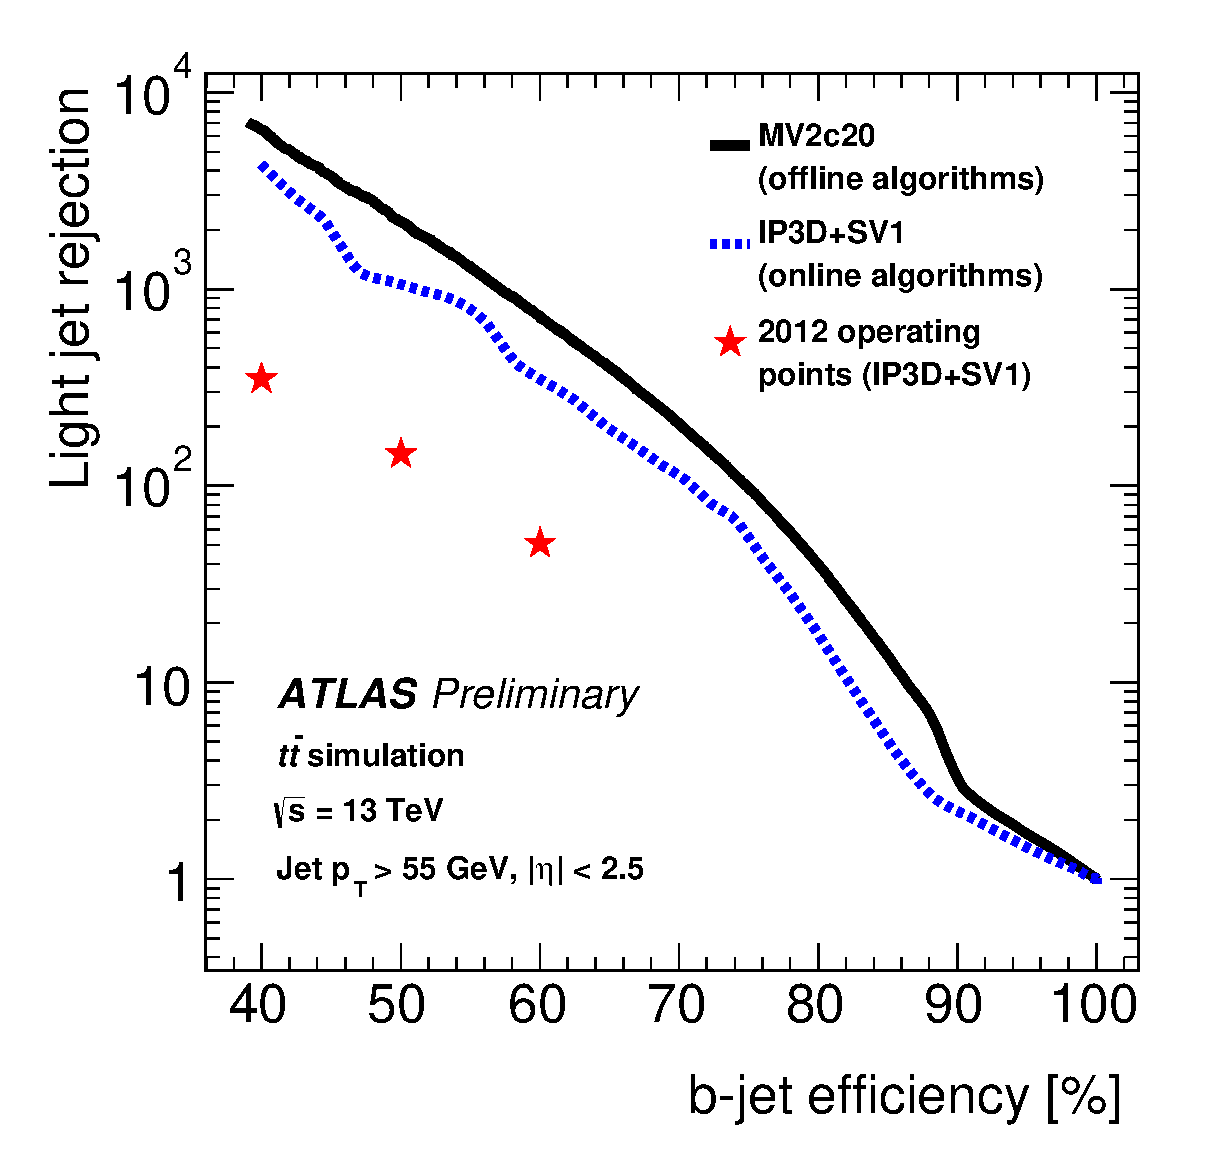
\includegraphics[width=0.48\linewidth, angle=0]{figs/Trigger/trig-bTrig_perf_light.eps}
    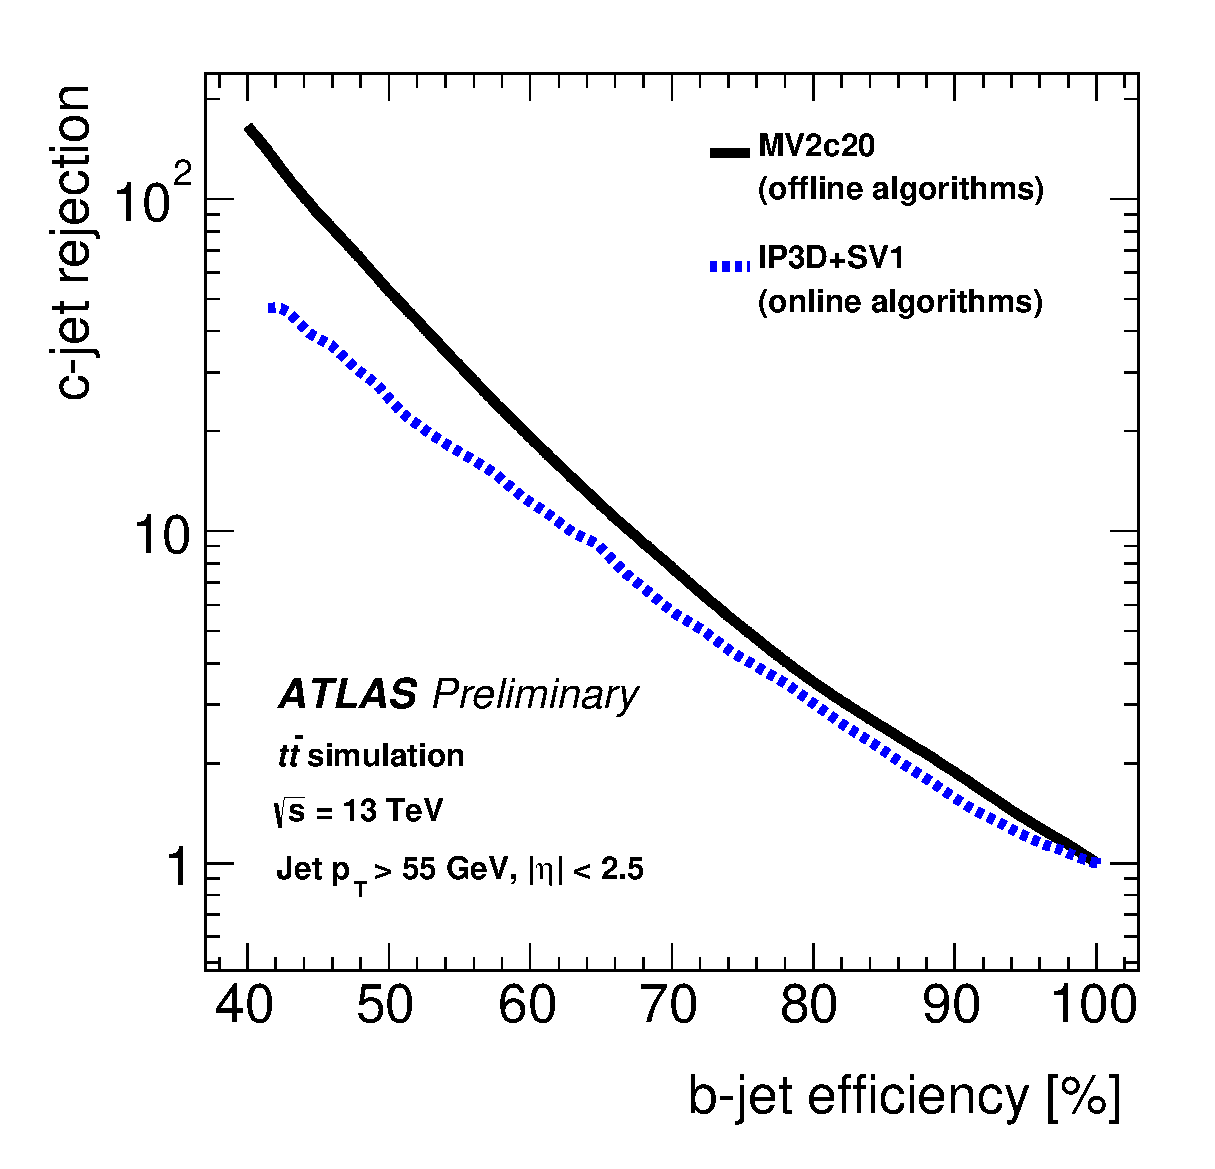
\includegraphics[width=0.48\linewidth, angle=0]{figs/Trigger/trig-bTrig_perf_charm.eps}
  \end{center}
  \caption[The expected $b$-jet efficiency of $b$-jet triggers with respect to (a) light-jet and (b) $c$-jet rejection
    in the case where the $b$-tagging algorithm used is MV2c20 (Black), IP3D+SV1 (Blue) and for the set-up used in Run-1 (red stars)]
    {The expected $b$-jet efficiency of $b$-jet triggers with respect to (a) light-jet and (b) $c$-jet rejection
    in the case where the $b$-tagging algorithm used is MV2c20 (Black), IP3D+SV1 (Blue) and for the set-up used in Run-1 (red stars)~\cite{trig-bTrig_desc}.}
  \label{fig:trig-bTrig_perf}
\end{figure}

There are few subtleties worth commenting on the $b$-jet trigger configuration which affect decisions taken in this analysis.
One is that on this figure there are two lines corresponding to different $b$-tagging algorithms used in $b$-jet trigger;
IP3D+SV1 was used in 2015 data-taking,
whilst the MV2c20 was used in 2016 data-taking.
Another difference between 2015 and 2016 is the primary vertex finding algorithm used;
2016 data-taking employed an algorithm based on offline primary vertex finding, know as \verb|xPrmVtx|,
whilst in 2015 an algorithm using a simpler histogram based approach was employed, known as \verb|EFHist|. 

Finally it is worth noting that there are  differences between online and offline $b$-tagging that will have an impact on what is to follow.
Firstly, coarser tracking information is available online, notably online tracks are not reconstructed from the whole range of the detector.
Secondly, a slightly different training setup is used for the multi-variate algorithm, mainly that a different fraction of $c$-jets were present in the training sample
(10\% offline vs. 20\% online).

In this analysis a double $b$-jet trigger is used,
\begin{center}
\verb|HLT_j150_bmv2c2060_split_j50_bmv2c2060_split|
\end{center}
which triggers on two jets with $p_T >$ 150 and 50 GeV respectively,
which have been $b$-tagged at the 60\% efficiency working point.

\newpage

\section{Efficiency Measurement of the $b$-Jet Trigger}
\label{sec:trig-bjet_eff}

Any part of the ATLAS detector framework needs to be understood and calibrated with data for use in an analysis;
and this includes the trigger which can have a large impact on the analysis.
In this section I discuss the strategy and results of the $b$-jet trigger efficiency measurement in 2016,
which is an important input to the low-mass channel of the di-$b$-jet analysis.

For clarity in this section I would like to make two definitions clear.
Online refers to any algorithms run or objects reconstructed at the trigger level,
offline refers to algorithms run after events have passed the trigger at the data-processing level. 

\subsection{Strategy}
The $b$-jet trigger is always used in tandem with offline $b$-tagging which is calibrated independently of the $b$-trigger.
As mentioned before, there are many differences between offline and online $b$-tagging.
Hence, to do this measurement whilst making use of the offline $b$-tagging calibrations already available,
$b$-jet trigger efficiency with respect to offline $b$-tagging, $\epsilon_{bTrig}$, is measured.
This is defined as the number of offline-tagged true $b$-jets that match an online-tagged trigger-jet
divided by the number of offline tagged $b$-jets that match a trigger jet.
Or to put this in an equation;
\begin{equation}
 \epsilon_{bTrig} = \frac{N(\text{Offline-tagged, online-tagged, true $b$-jets)}}{N(\text{Offline-tagged, trigger-matched, true $b$-jets)}}
\end{equation}
This quantity can be interpreted as the probability that a true $b$-jet is tagged at the trigger-level,
given that it there is a jet at the trigger level and that it would be $b$-tagged at the offline stage.

To measure $\epsilon_{bTrig}$ a sample that has high $b$-jet purity is required,
such that jets used to calculate this ratio are true $b$-jets.
It is also necessary to trigger on this sample in such a way that there is no bias from using $b$-tagging online;
or simply put the $b$-jet trigger cannot be used to select events.
The sample used to fill these criteria is a di-lepton $t\bar{t}$ sample containing a muon and an electron.
Top-quarks decay to a $W$-boson and a $b$-quark with almost 100\% branching ratio meaning that this sample provides a good source of $b$-quarks,
but also the electron and muon give a distinct signature which allows us to select this process with good purity and gives a non-$b$-jet object to trigger on.
The exact event selection is described below. 

The $b$-jet trigger efficiency is determined in data and is compared to the efficiency found in a 
simulated $t\bar{t}$ sample which is used to extrapolate the efficiency to 
higher jet-$p_T$ where the data-derived efficiency loses statistical precision.
The efficiency in data, including the simulation based extrapolation, can then be
compared to simulation to derive a Data/Monte-Carlo scale factor, which is used as the input to the analysis.


$\epsilon_{bTrig}$ and Data/Monte-Carlo scale factors are derived for all combinations of offline and online $b$-tagging working points.
However, only the process for the 70\% offline and 60\% online working point is shown
as this is set of working points used in this analysis.

\subsection{Datasets}
The data used for this analysis is the full 2016 ATLAS data-set.
In addition to the usual data-quality requirements applied,
as discussed in Section~\ref{sec:evtSel_GRL}\textit{(sec:evtSel\_GRL)},
a $b$-jet trigger aware Good Run List (GRL)
\footnote{A GRL is effectively a list of lumi-blocks that pass certain data-quality requirements.
 As mentioned in the text a further discussion is held here in Section~\ref{sec:evtSel_GRL}\textit{(sec:evtSel\_GRL)}}
applies the requirement that the online beamspot $z$-position is within 2mm of the origin in Periods A-I of the data.
This means that the data-set contains 24.5~\ifb~of data.
A discussion of the requirement for this GRL is in Section~\ref{sec:trig-inv}. 

For the simulated $t\bar{t}$ sample, the generation is performed with
a Powheg-Box v2~\cite{trig-powheg} generator with the CT10 PDF sets in the matrix element calculations.
Also considered is a simulated single-top sample;
electroweak t-channel, s-channel and $Wt$-channel single top-quark events are generated using the Powheg-Box v1 generator.
This generator uses the 4-flavour scheme for the NLO matrix elements calculations together with the fixed four-flavour PDF set CT10f4.
%For all top processes, top-quark spin correlations are preserved (for t-channel, top quarks are decayed using MadSpin[10a]).
For both processes the parton shower, fragmentation, and the underlying event are simulated using Pythia6.428~\cite{trig-pythia6} with the CTEQ6L1~\cite{trig-CTEQ6L1} PDF sets
and the corresponding Perugia 2012 tune (P2012)~\cite{trig-perugia}.
The top mass is set to 172.5 GeV.
The EvtGen v1.2.0 program~\cite{trig-evtGen} is used for properties of the bottom and charm hadron decays. 
\newpage

\subsection{Event Selection}
\label{sec:trig-evtSel}

A high-purity sample of $b$-jets is selected using a di-lepton $t\bar{t}$ selection.

\noindent
The event selection is summarised as follows:

\begin{itemize}
\item The event fired a single lepton bperf trigger which are:
    \begin{itemize}[label={$-$}]
      \item\verb|HLT_mu26_imedium_2j35_bperf|
      \item\verb|HLT_e26_tight_iloose_2j35_bperf|
      \item\verb|HLT_e26_lhtight_iloose_2j35_bperf|
    \end{itemize}
\item At least 1 medium muon: $\pT>25~\GeV$, which has no jet within a $\Delta R$ of 0.4.
\item At least 1 medium electron: $\pT>25~\GeV$.
\item 2 offline $b$-tagged jets, defined as:
   \begin{itemize}[label={$-$}]
     \item Offline R=0.4 anti-$k_T$ jets.
     \item $\pT>35~\GeV$ and $|\eta|<2.5$.
     \item Offline $b$-tagged at the 85\%~operating point.
     \item Jet must be matched to a trigger-jet.
    \end{itemize}
\end{itemize}
\vspace{1em}

Descriptions of the object-definitions of muons, electrons, jets and $b$-tagged can be found in
Sections~\ref{sec:object_muon}\textit{(sec:object\_muon)},~\ref{sec:object_electron}\textit{(sec:object\_elec)},~\ref{sec:object_jet}\textit{(sec:object\_jet)}
and \ref{sec:object_bjet}\textit{(sec:object\_bjet)} respectively.
Online trigger jets are matched exclusively to offline jets using $\Delta R$ matching, requiring for a match the jets must have $\Delta R<0.6$.

The triggers used are bperf trigger, which are special triggers used in data-taking specifically for monitoring the $b$-jet trigger performance.
They fire if a muon or an electron with $\pT > 26$~\GeV~is reconstructed at the trigger level.
The bperf triggers then run the online $b$-tagging algorithm on all trigger jets with $|\eta|<2.5$ and
$p_{T}>35$~\GeV~without performing any cuts on the output of the multi-variate algorithm; ensuring there is no bias in the efficiency measurement. 


\newpage

\subsection{The Initial Problem}
\label{sec:trig-initProb}

To give context to the following section;
the first discussion will be what was first observed when measuring the $b$-jet efficiency.
To show the problems observed clearly, in this section the initial event selection is replicated;
hence  no $b$-jet trigger aware GRL is applied, offline jets are not required to match a trigger jet in the denominator
and the triggers required are single lepton triggers without the additional $b$-perf functionality
\footnote{Specifically HLT\_mu26\_imedium, HLT\_e26\_tight\_iloose and HLT\_e26\_lhtight\_iloose. }.
In addition, for this and the following two sections simulation refers to $t\bar{t}$ only,
but it will be shown later that the effect of single-top production is small so the conclusions here are still valid. 

Figure~\ref{fig:trig-Full_noGRL_eff_noHLTMatch} shows $\epsilon_{bTrig}$ against jet-\pT~and jet-$\eta$;
the efficiency in data is substantially below the efficiency expected from simulation and shows a clear shape in jet-$\eta$ distributions.
This substantial differences need to be investigated and understood. 

\begin{figure}[!ht]
  \begin{center}
    \captionsetup[subfigure]{aboveskip=0pt,justification=centering}
    \subcaptionbox{Jet-\pT}{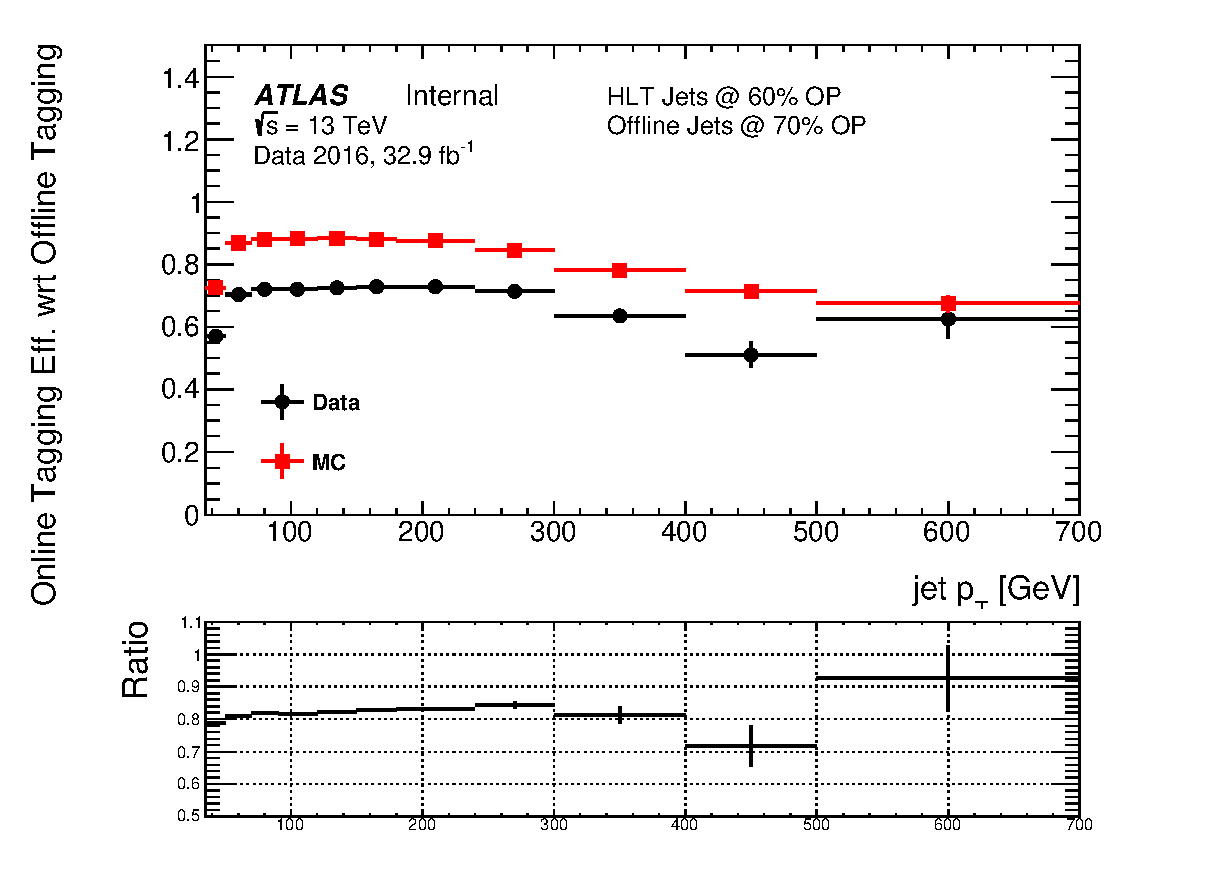
\includegraphics[width=0.48\linewidth, angle=0]{figs/trigger/Full_noGRL_eff_noHLTMatch_jetPt.eps} }
    \subcaptionbox{Jet-$\eta$}{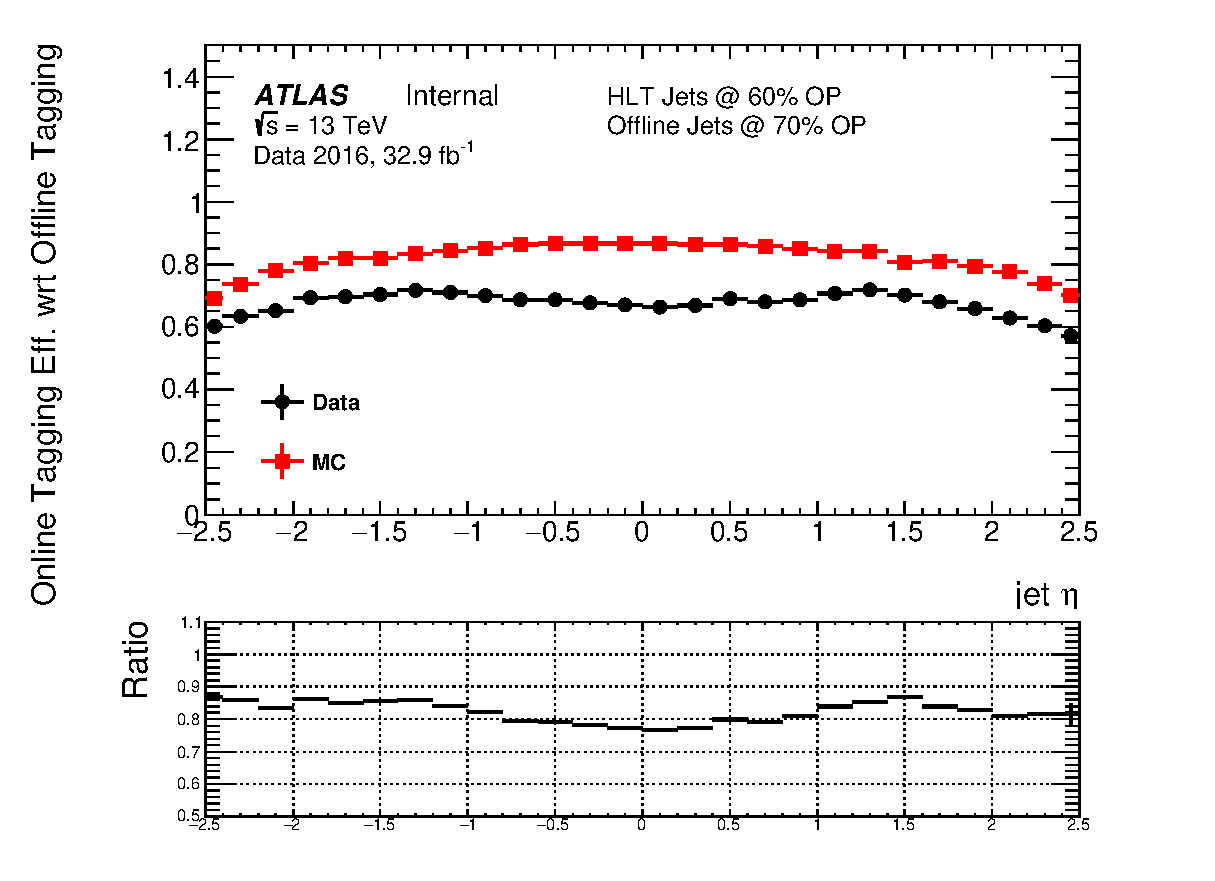
\includegraphics[width=0.48\linewidth, angle=0]{figs/trigger/Full_noGRL_eff_noHLTMatch_jetEta.eps}}
  \end{center}
  \caption{The 60\% $b$-jet trigger efficiency with respect to an offline 70\% operating point tag
    for Data (black) and simulation (red) against jet-\pT~(a) and jet-$\eta$ (b).
    The $b$-trigger aware GRL is not applied and trigger matching is not required.}
  \label{fig:trig-Full_noGRL_eff_noHLTMatch}
\end{figure}

\subsection{Investigation}
\label{sec:trig-inv}

Given the disagreements between data and simulation shown above
a number of cross-checks were performed to understand this discrepancy,
including checking for performance dependence on period,
detector performance, pile-up conditions and online beamspot position.
In this section, I summarise the results of the investigation
and our understanding of the $b$-trigger performance in 2016 data.
For this, the set-up as described in \ref{sec:trig-evtSel} is used
with the exception that the $b$-jet aware GRL is not applied to allow us to see the problems clearly.

The major problem that was discovered to be causing the large discrepancies was related to primary vertex finding.
As described above, in 2016 data an algorithm known as \verb|xPrmVtx| was used to find the primary vertex.
It has since been uncovered that there was a bug in the code used to implement this algorithm;
effectively different co-ordinates were used by different components of the code.
Online tracks passed to \verb|xPrmVtx| use position with respect to online beam-spot position,
where the \verb|xPrmVtx| algorithm assumed track position with respect to the origin.
This means that when the online beamspot $z$-position is far from from the origin,
a dummy vertex with position at the origin is passed to the $b$-tagging algorithms.
This leads to sub-optimal performance, as will be shown below.
For ease of reading online beamspot $z$-position is henceforth referred to as $z_{bs}^{online}$.  

The exact setup for the $b$-jet trigger has changed as data has been taken, to respond to performance issues as they are noticed and patches are applied.
As such the relevant conditions of the $b$-jet trigger can be split into three regions of data-taking, which I will refer to as epochs.
The effect of \verb|xPrmVtx| returning a dummy vertex on $b$-jet trigger performance is different in each of these epochs,
the details are summarised Table~\ref{tab:trig-epochs}.
As a result of these differences in trigger performance, each epoch is now considered independently.

\begin{table}[!htb]
  \begin{tabular}{ | c || c | c | c |}
    \hline			
    Epoch & Runs & Periods & Effect if no \verb|xPrmVtx| PV is found \\ \hline
    1 & \parbox[t]{2.5cm} {296939-300571,\\ 300655 \\}  & A,B(part)             & \parbox[t]{5cm} {\hspace{1mm}An invalid vertex is passed to the online b-tagging } \\
    \hline
    2 & \parbox[t]{2.5cm} {300600,\\ 300784-308084\\}  & B(part),C,D,E,F,G,I,J & \parbox[t]{5cm} {\hspace{1mm}The b-jet trigger is not fired\\ } \\
    \hline
    3 & \parbox[t]{2.5cm} {309331-311481\\}       & K,L                     & \parbox[t]{5cm} {\hspace{1mm}A back-up primary vertex \\ finding algorithm is used.\\} \\
    \hline
  \end{tabular}
  \vspace{10pt}
  \caption{A table describing the effect of not finding a valid xPrmVtx primary vertex on different epochs of data.}
  \label{tab:trig-epochs}
\end{table}
%For Epoch 1, the $\epsilon_{bPerf}$ is 100\% as shown in Figure~\ref{fig:Epoch1_bperf} for Period A.Figure~\ref{fig:Epoch1_eff} shows the $\epsilon_{bTrig}$ in Epoch 1,
Firstly let us consider Epoch 1;
Figure~\ref{fig:Epoch1_eff}(a) shows that efficiency against jet-\pT~is ~80-90\% of that in simulation, similar to that shown in the previous section.
However, Figure~\ref{fig:Epoch1_eff}(b) shows that $\epsilon_{bTrig}$ in Epoch 1 has a strong dependence of  $z_{bs}^{online}$;
when  $z_{bs}^{online}$ is close to zero $\epsilon_{bTrig}$ in data and simulation are comparable
\footnote{In simulation the  $z_{bs}^{online}$ is always set to zero.}
but as $|z_{bs}^{online}|$ increases efficiency falls off steeply.
To understand this performance the variable `vertex class' is studied, which is defined as 0 when a valid \verb|xPrmVtx| vertex is found and 1 if not.
Figure~\ref{fig:Epoch1_vtxClass}(a) shows that when an \verb|xPrmVtx| vertex is found $\epsilon_{bTrig}$ is reasonably high ($\sim$ 0.8) and is comparable between data and simulation (within 5\%),
whilst if no valid \verb|xPrmVtx| vertex is found then efficiency is very low in both simulation and data.
However, Figure~\ref{fig:Epoch1_vtxClass}(b) shows that a valid \verb|xPrmVtx| vertex is found in simulation in $> 99$ \% of the jets,
whilst in data there is $\sim$ 16\% of events where no valid \verb|xPrmVtx| vertex is found.
Hence, combining the information in Table~\ref{tab:trig-epochs}, Figure~\ref{fig:Epoch1_eff} and Figure~\ref{fig:Epoch1_vtxClass}
it can be concluded that in Epoch 1 in events where the  $|z_{bs}^{online}|$ is far from 0
then \verb|xPrmVx| returns an dummy vertex which results in a low $\epsilon_{bTrig}$, explaining the data/simulation differences in Epoch 1. 

\begin{figure}[!ht]
  \begin{center}
    \captionsetup[subfigure]{aboveskip=0pt,justification=centering}
    \subcaptionbox{Jet-\pT}{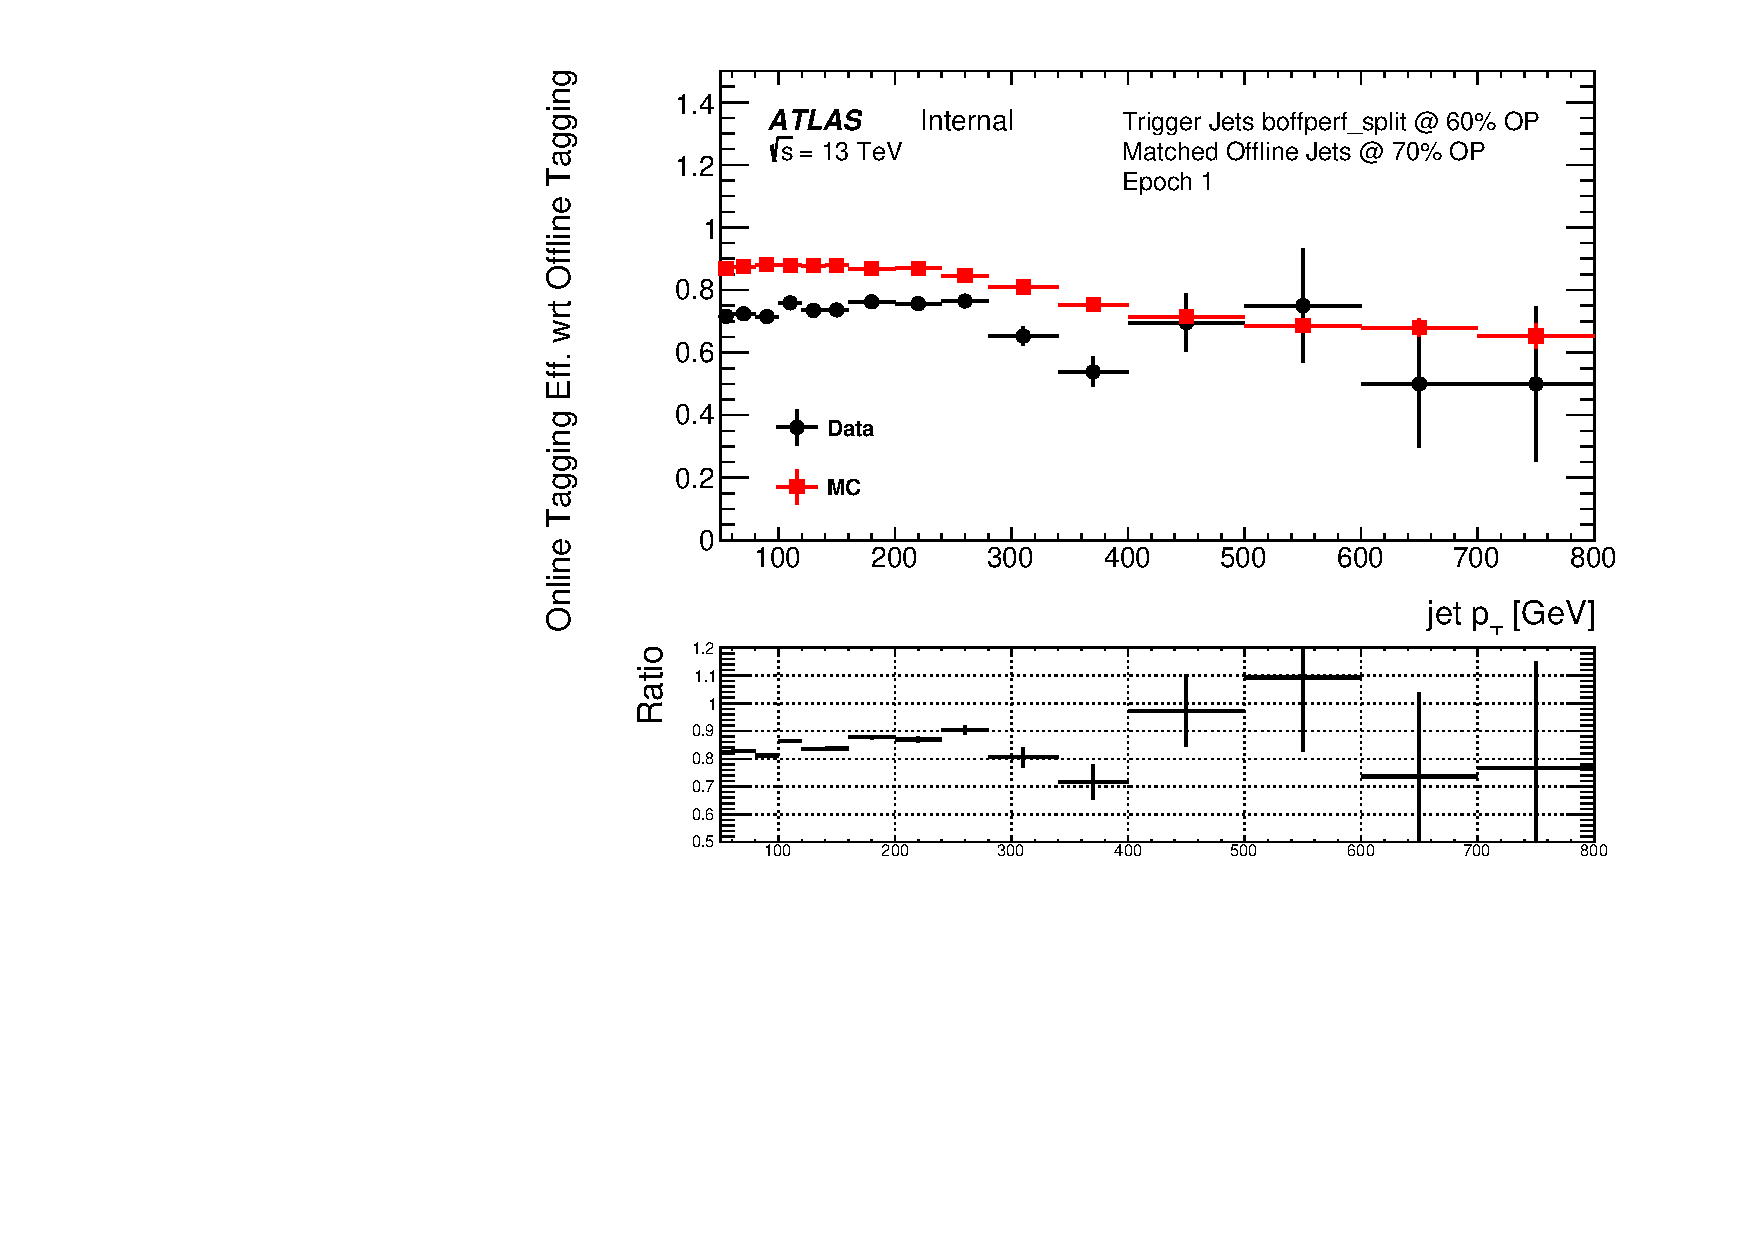
\includegraphics[width=0.48\linewidth, angle=0]{figs/Trigger/btrigger_old/Epoch1_trigReq_eff_jetPt.pdf} }
    \subcaptionbox{ $z_{bs}^{online}$}{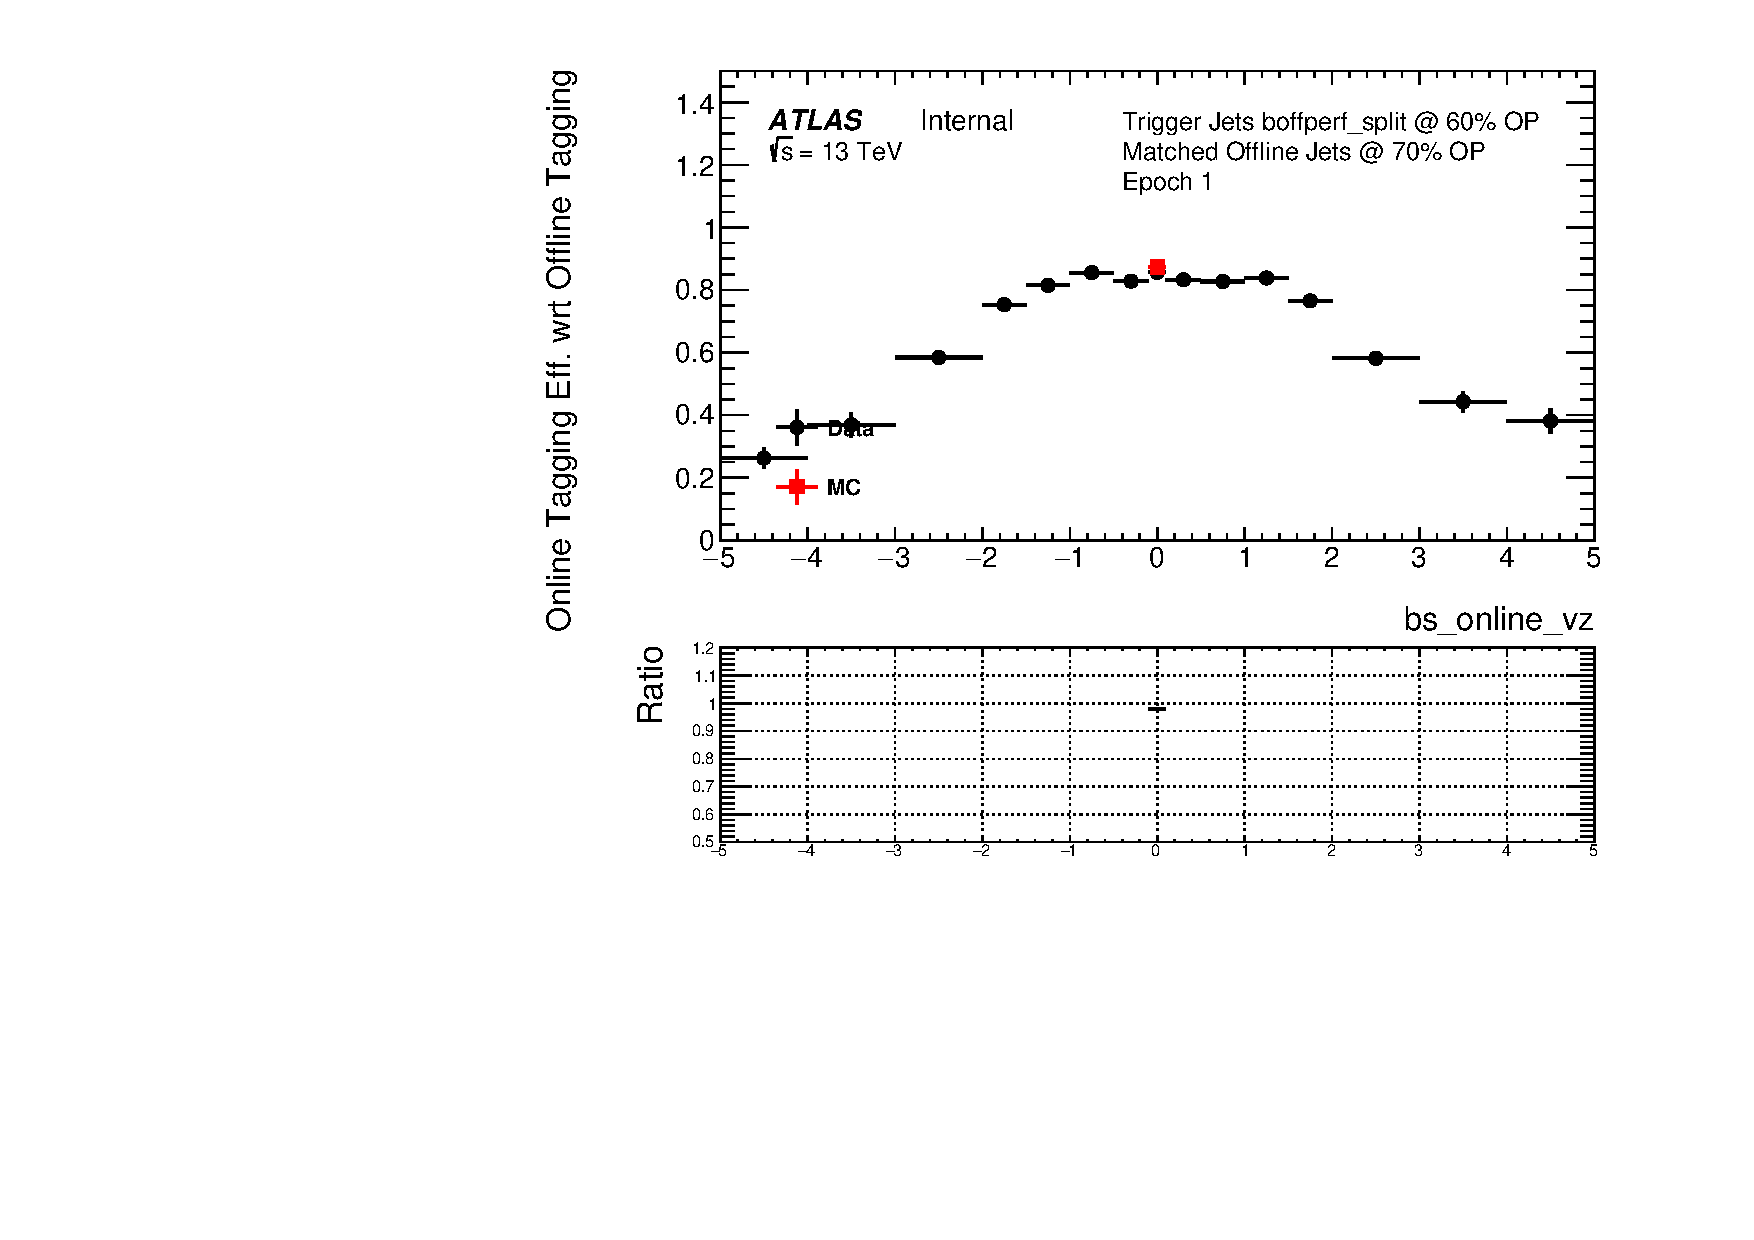
\includegraphics[width=0.48\linewidth, angle=0]{figs/Trigger/btrigger_old/Epoch1_trigReq_eff_bs_online_vz.pdf} }
  \end{center}
  \caption{The 60\% $b$-jet trigger efficiency with respect to an offline 70\% operating point tag
    for data from Epoch 1 (black) and simulation (red) against jet-\pT~(a) and online beamspot $z$-position (b).
    The $b$-jet trigger aware GRL has not been applied.}
  \label{fig:Epoch1_eff}
  \begin{center}
    \captionsetup[subfigure]{aboveskip=0pt,justification=centering}
    \subcaptionbox{$\epsilon_{bTrig}$ against Vertex Class}{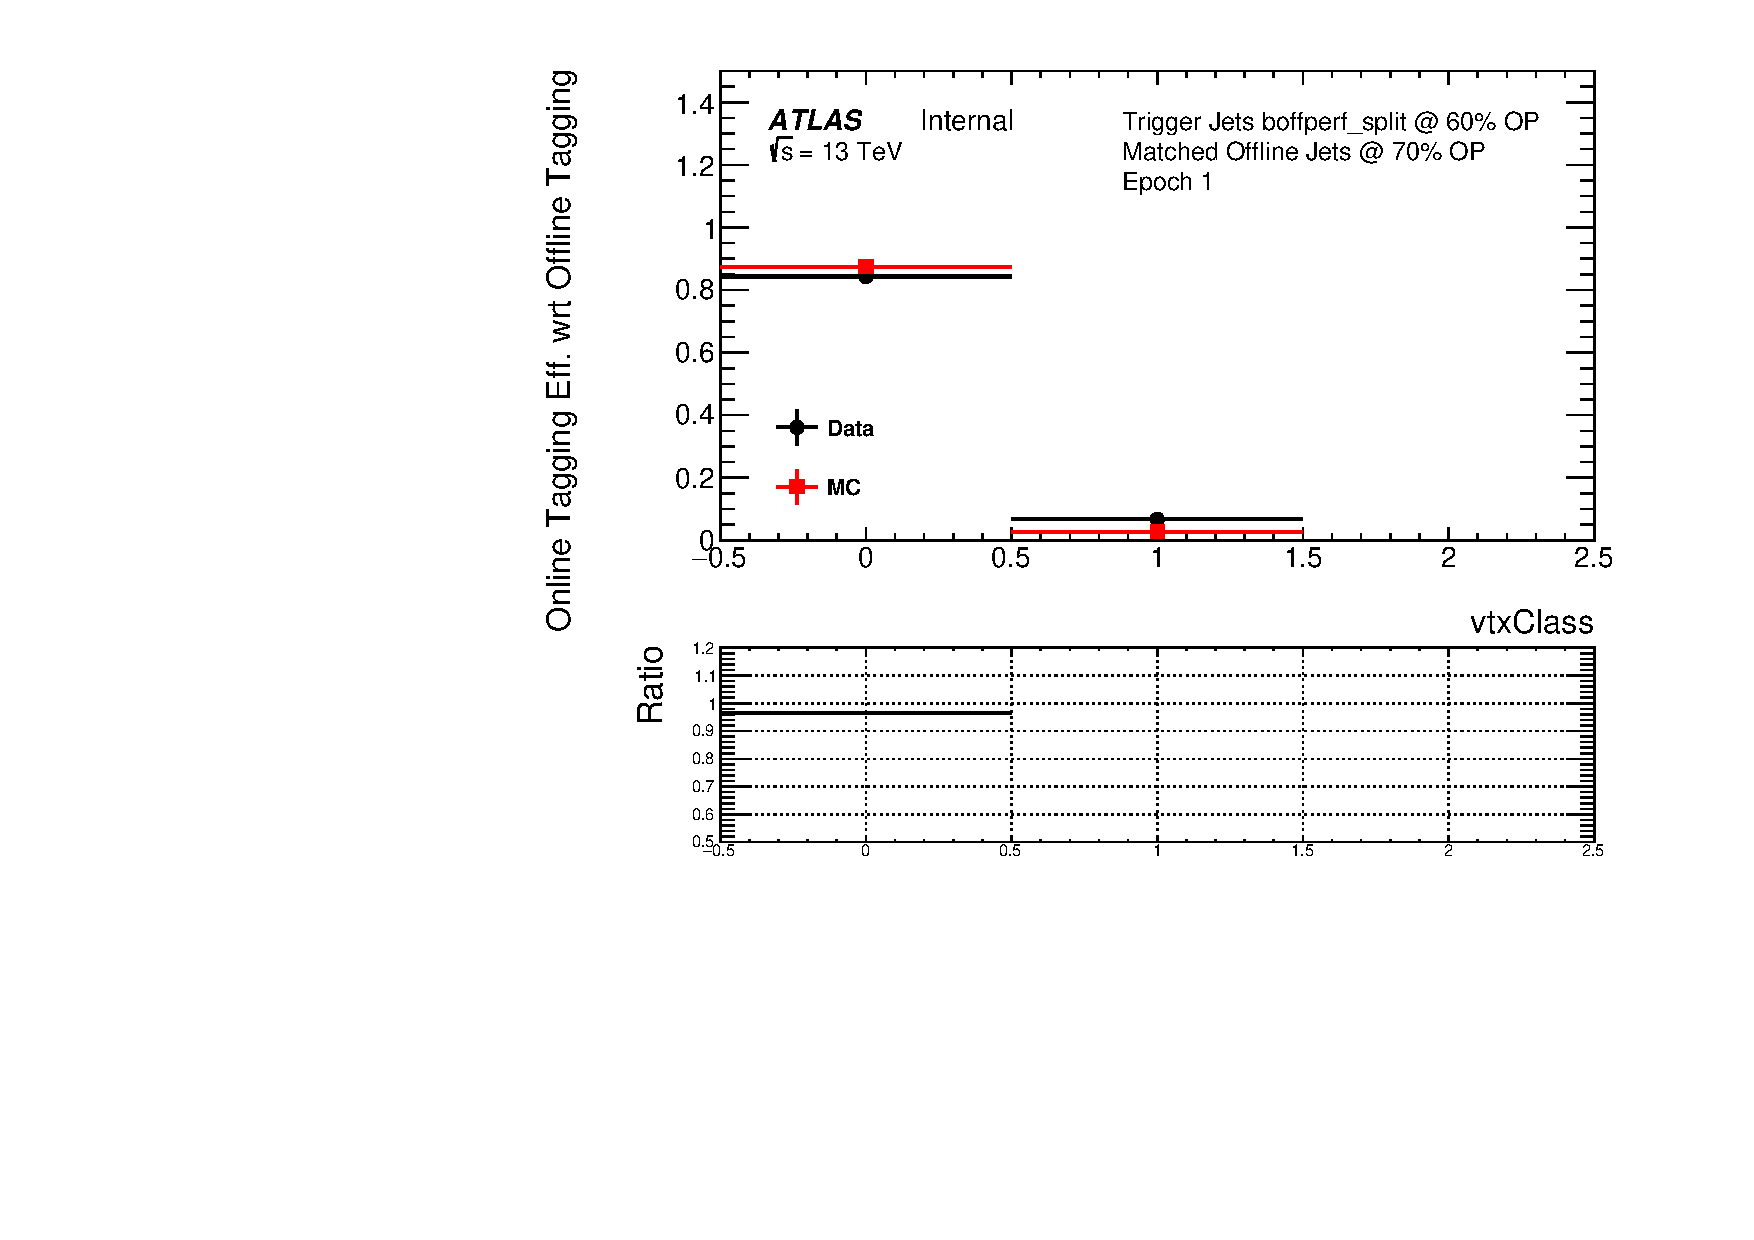
\includegraphics[width=0.48\linewidth, angle=0]{figs/Trigger/btrigger_old/Epoch1_trigReq_eff_vtxClass.pdf}}
    \subcaptionbox{Freq. of Offline Jets against Vertex Class}{\includegraphics[width=0.48\linewidth, angle=0]{figs/Trigger/btrigger_old/Epoch1_trigReq_nOff_vtxClass.pdf}}
    \end{center}
  \caption{(a) The 60\% $b$-jet trigger efficiency with respect to an offline 70\% operating point tag
    and  (b) the number of offline jets passing 70\% operating point tag and matching a HLT trigger jet
    against vertex class for data from Epoch 1 (black) and simulation (red). 
    The $b$-jet trigger aware GRL has not been applied.}
    \label{fig:Epoch1_vtxClass}
\end{figure}

\FloatBarrier


%\begin{figure}[!ht]
%\begin{center}
%  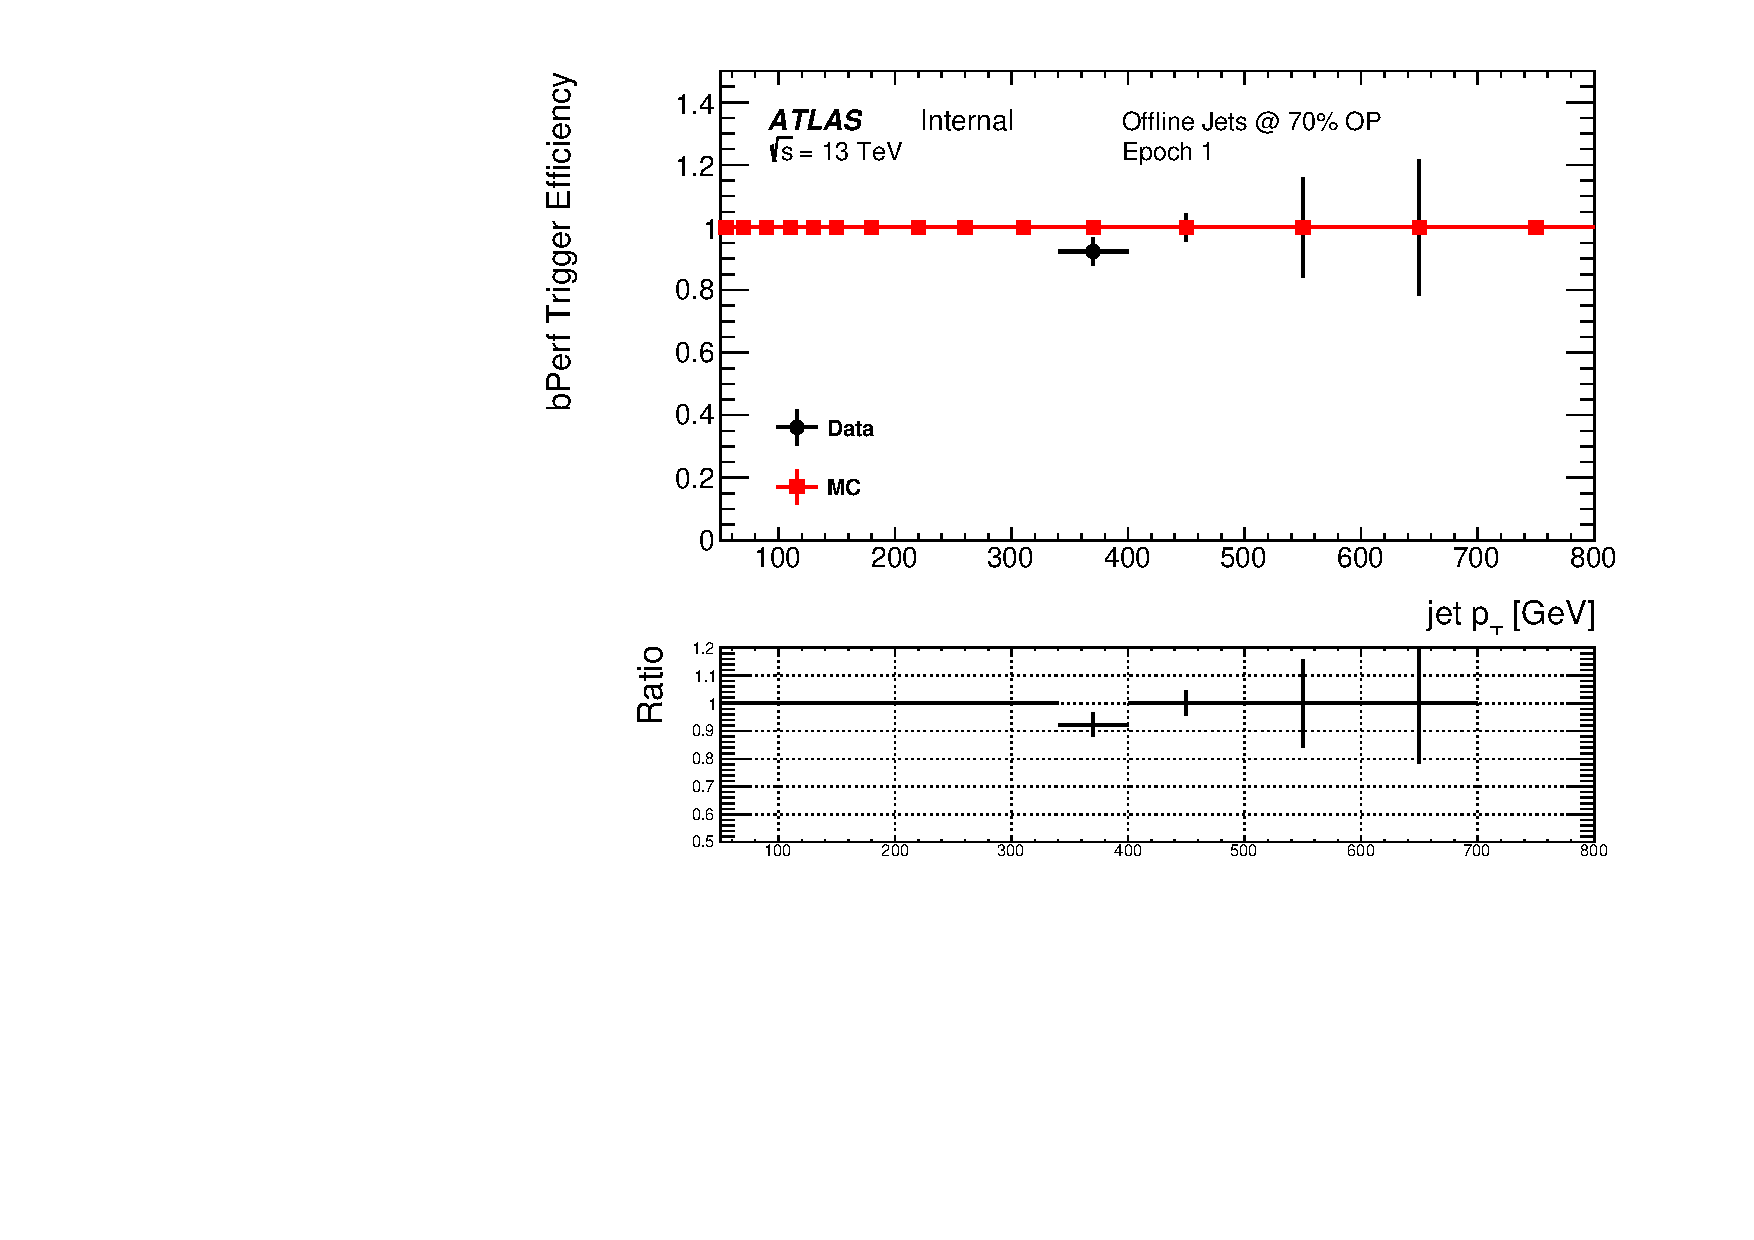
\includegraphics[width=0.47\linewidth, angle=0]{figs/Trigger/btrigger_old/Epoch1_trigReq_bPerfEff_jetPt.pdf}
%  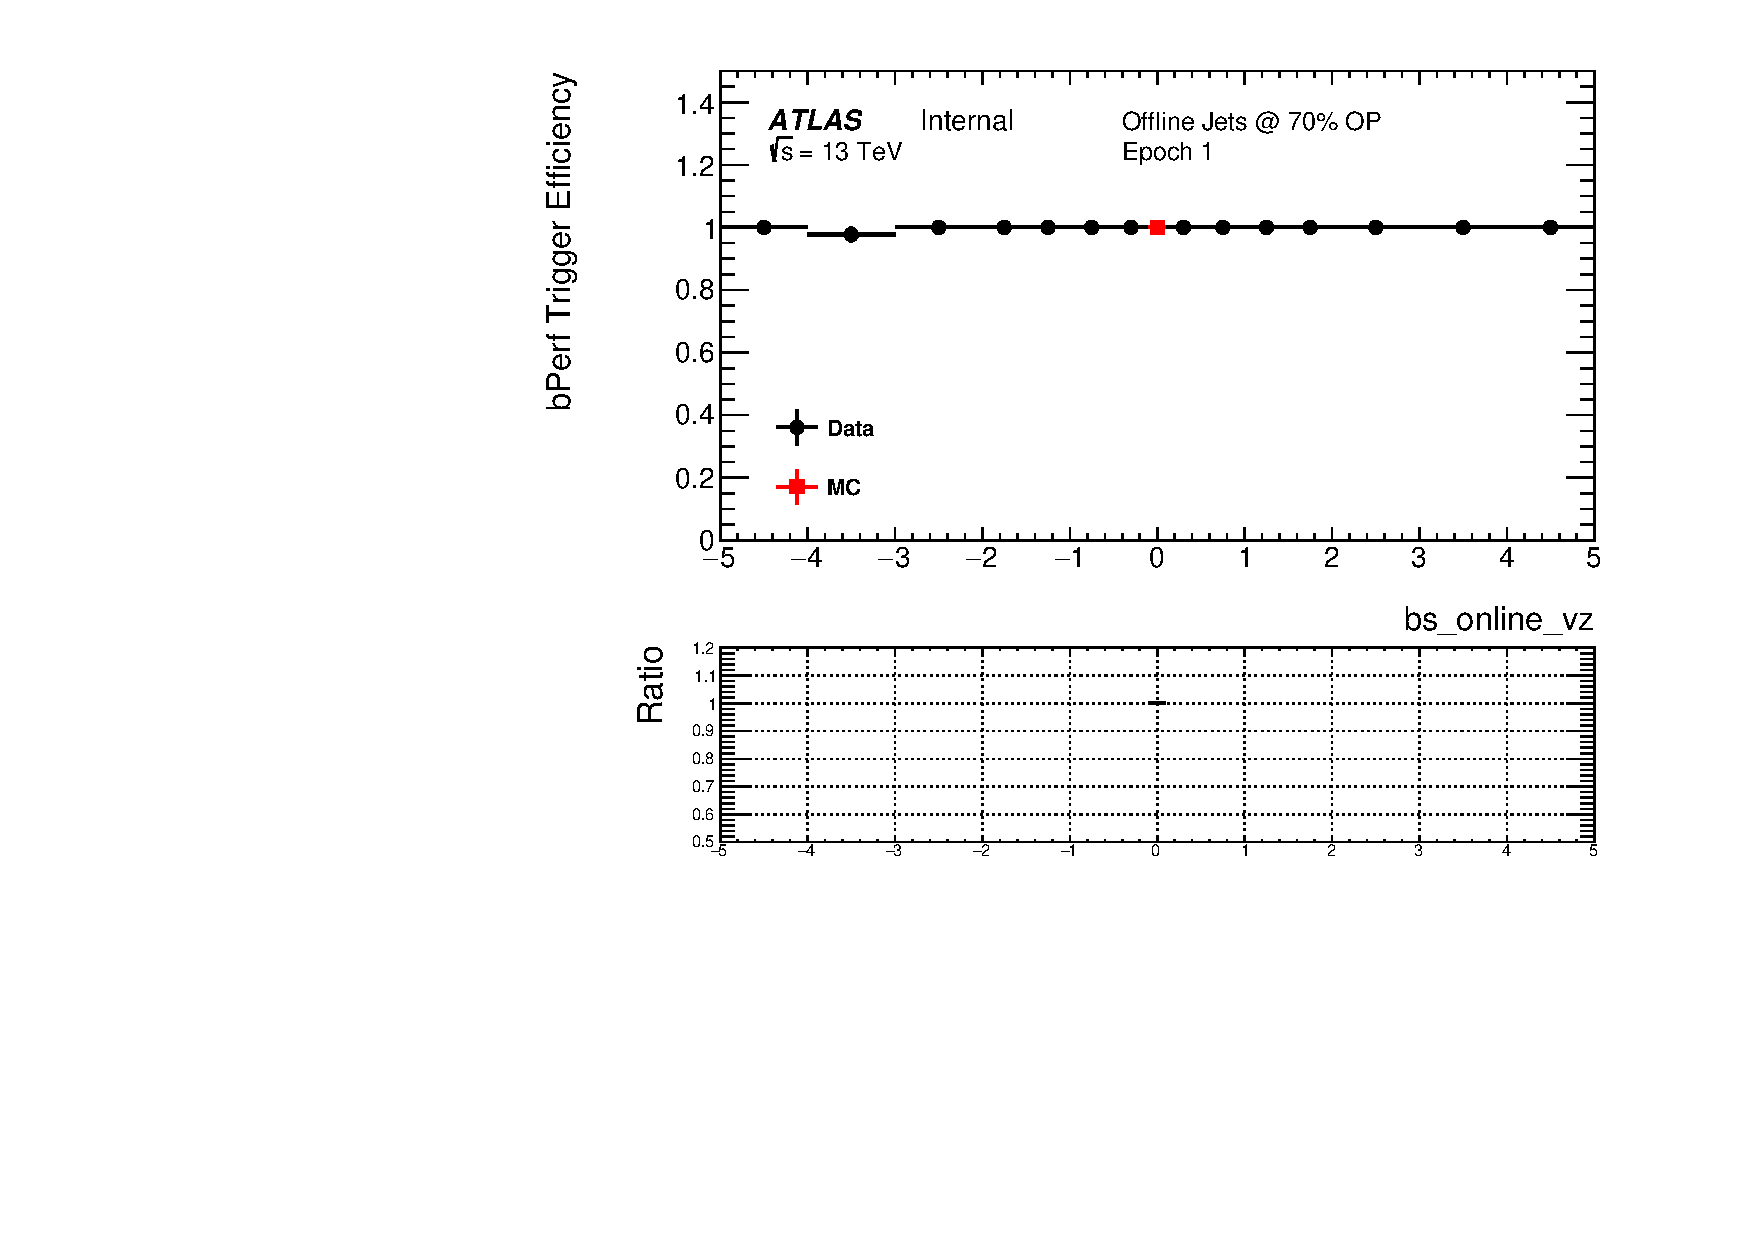
\includegraphics[width=0.47\linewidth, angle=0]{figs/Trigger/btrigger_old/Epoch1_trigReq_bPerfEff_bs_online_vz.pdf}
%\end{center}
%\caption{$b$-perf efficiency, $\epsilon_{bPerf}$, for data from Period A (black) and simulation (red) against jet-pT~(left) and online beamspot $z$-position (right).}
%\label{fig:Epoch1_bperf}
%\end{figure}

In Epoch 2, there is a similar problem to Epoch 1, but there is a subtle difference which requires us to look at this region in a
different way.
As in Epoch 1, when  $z_{bs}^{online}$ is far from zero then a \verb|xPrmVtx| PV is not found.
However in Epoch 2 this means that the  $b$-jet trigger was discovered to falsely terminate whilst processing the event,
meaning that there are no online $b$-jets are available in the event, and therefore the trigger will not fire.
However, the additional complication compared to Epoch 1 is this means that the  $b$-perf triggers used to measure the efficiency
are also not fired when no valid \verb|xPrmVtx| PV is available.
Hence, measuring $\epsilon_{bTrig}$ using the set-up as described will not capture the cases where a valid \verb|xPrmVtx| PV is found
and thus $\epsilon_{bTrig}$ should be consistent in data and simulation;
Figure~\ref{fig:Epoch2_eff} shows that the $\epsilon_{bTrig}$ measured in data to be in agreement with simulation within 5\%.


For Epoch 2, in addition to measuring $\epsilon_{bTrig}$ it is necessary
to also account for the cases when a false \verb|xPrmVtx| PV is found.
This is done by measuring the $b$-perf efficiency, $\epsilon_{bPerf}$,
the efficiency that there is a valid primary vertex in the event.
$\epsilon_{bPerf}$ is calculated by dividing the number of events that pass the trigger
\verb|HLT_mu26_imedium_2j35_bperf| by the number that pass the trigger \verb|HLT_mu26_imedium|,
such that the denominator has no $b$-trigger dependency so is unaffected by \verb|xPrmVtx| PV.
This is an event level quantity and as such is measured with respect to other event level quantities, such as leading jet-\pT.
Figure~\ref{fig:Epoch2_bperf} shows that:
$\epsilon_{bPerf}$ has a data/simulation ratio of around 80\%  which is similar to that in Section~\ref{sec:trig-initProb} and
$\epsilon_{bPerf}$ shows similar behaviour with respect to  $z_{bs}^{online}$ as observed in Epoch 1.
Finally it is observed that $\epsilon_{bPerf}$ has a lower efficiency at smaller values of absolute leading jet-$\eta$;
this is due to the fact that at high-$\eta$ tracks have a larger error on the longitudinal impact parameter, $z_0$,
meaning that the mis-match of co-ordinates can in the \verb|xPrmVtx| algorithm is covered by the errors, mitigating this issue.
This effect must be accounted for in the final efficiency measurement.\textbf{This last two sentances are dodgy}

\begin{figure}[!ht]
\begin{center}
  \captionsetup[subfigure]{aboveskip=0pt,justification=centering}
  \subcaptionbox{Jet-\pT}{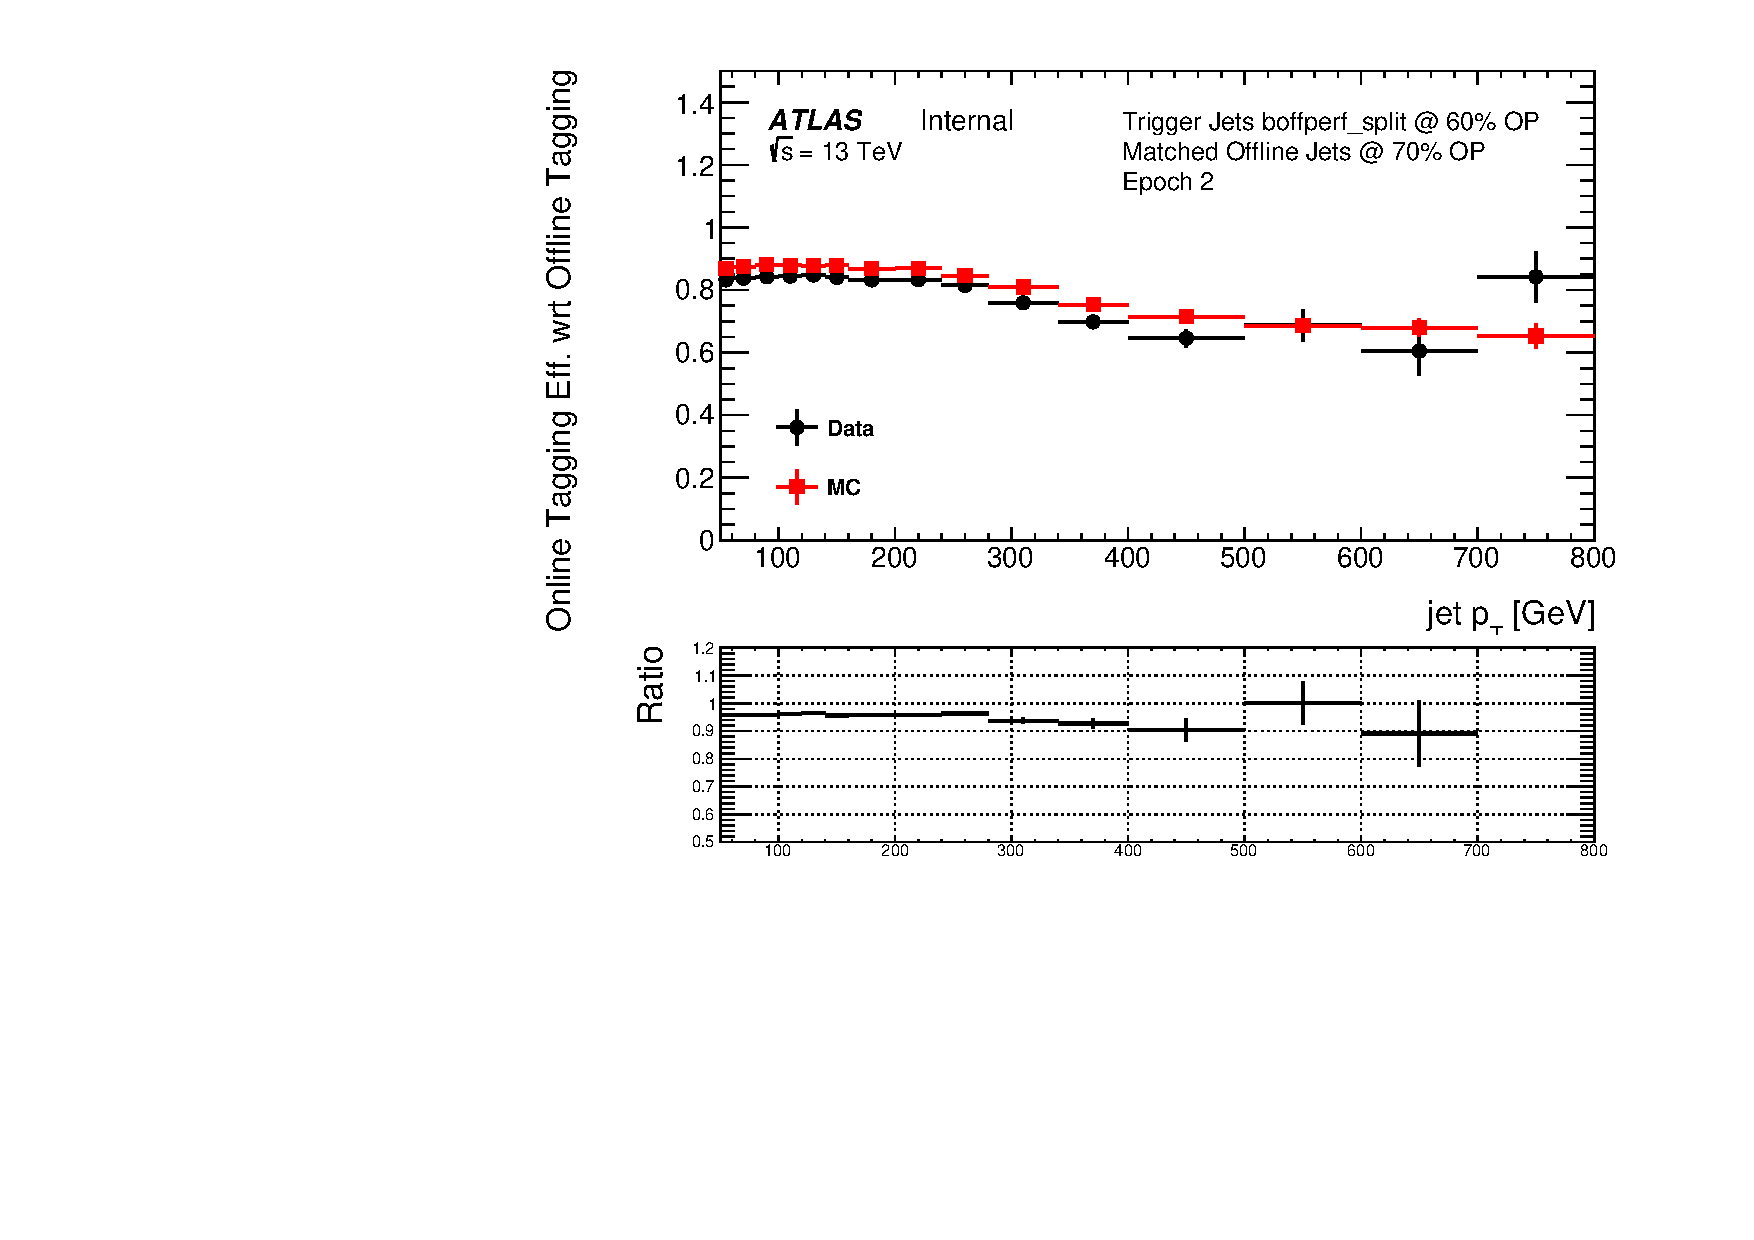
\includegraphics[width=0.47\linewidth, angle=0]{figs/Trigger/btrigger_old/Epoch2_trigReq_eff_jetPt.pdf}}     
  \subcaptionbox{Jet-$\eta$}{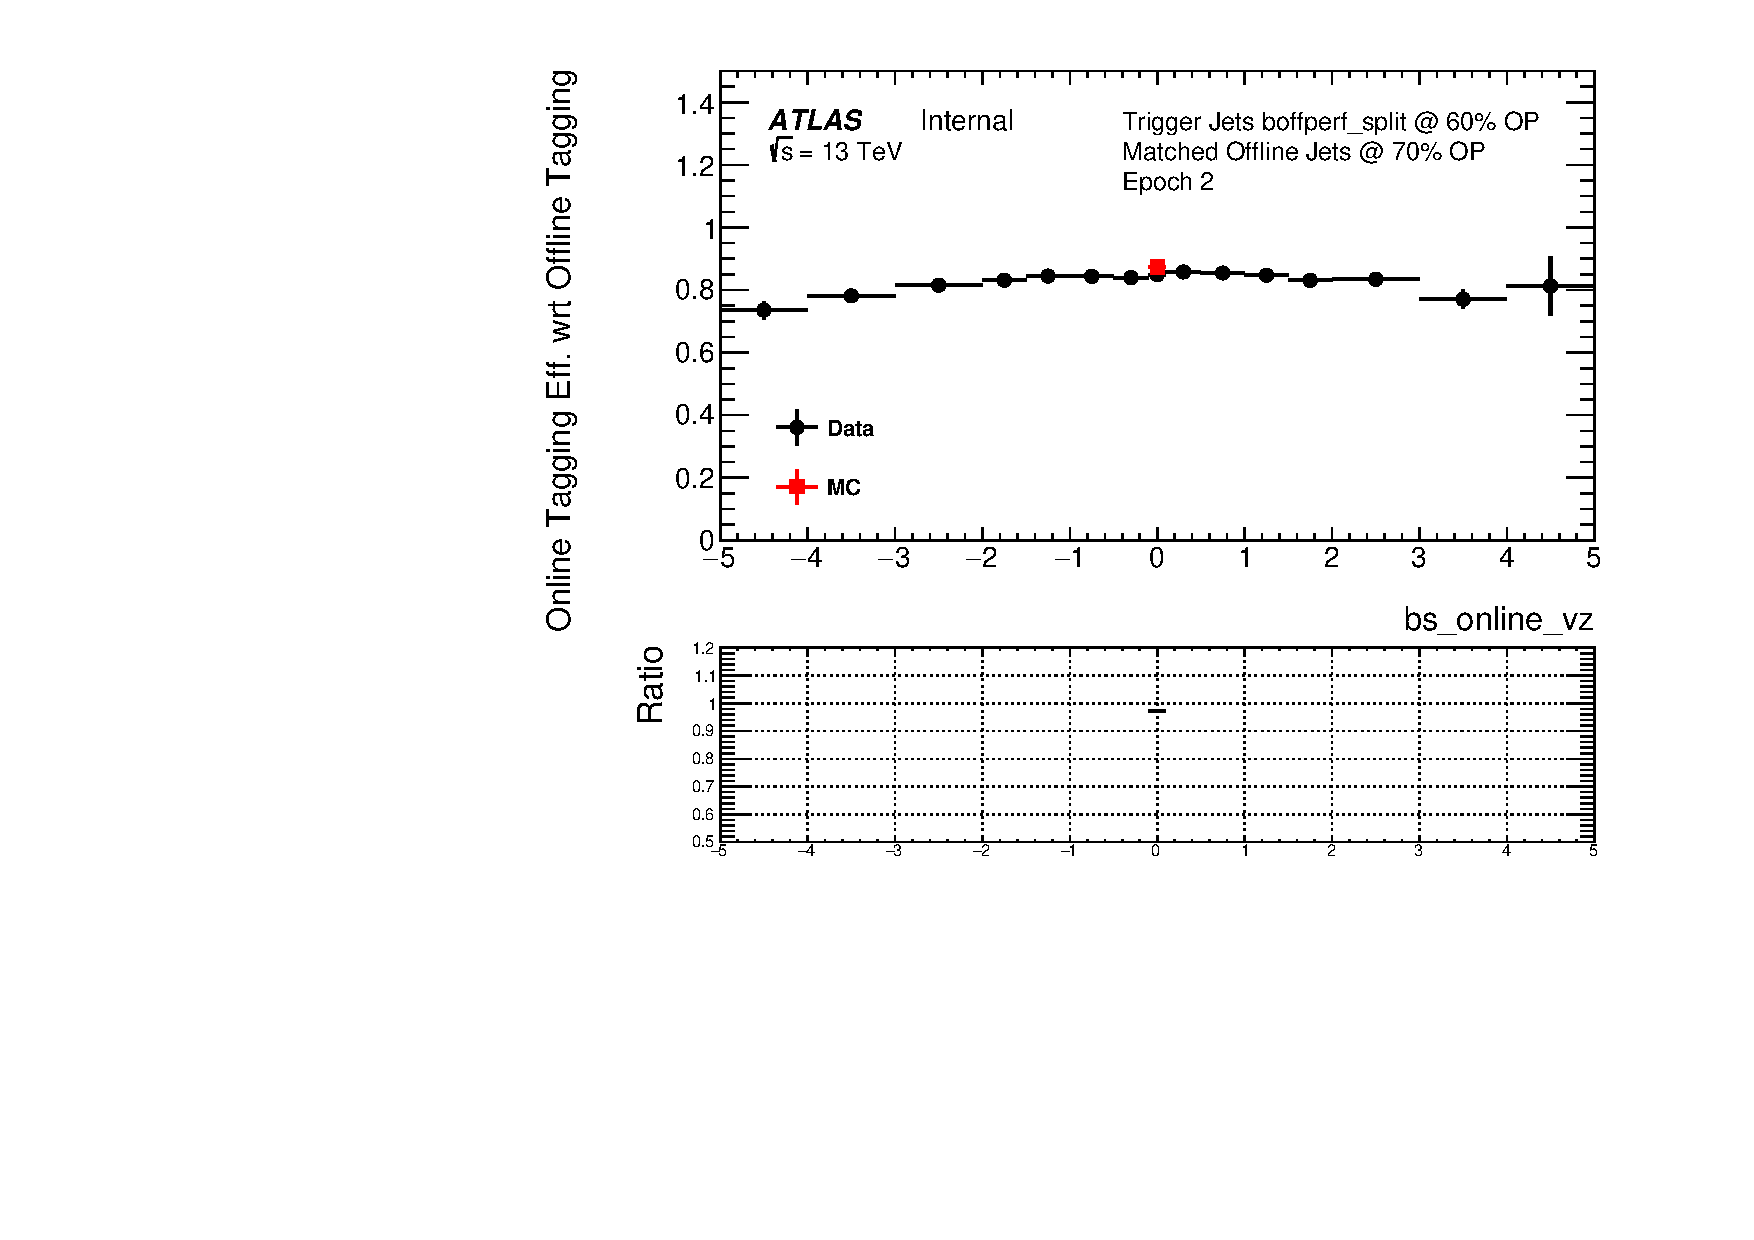
\includegraphics[width=0.47\linewidth, angle=0]{figs/Trigger/btrigger_old/Epoch2_trigReq_eff_bs_online_vz.pdf}}
  %\subcaptionbox{??}{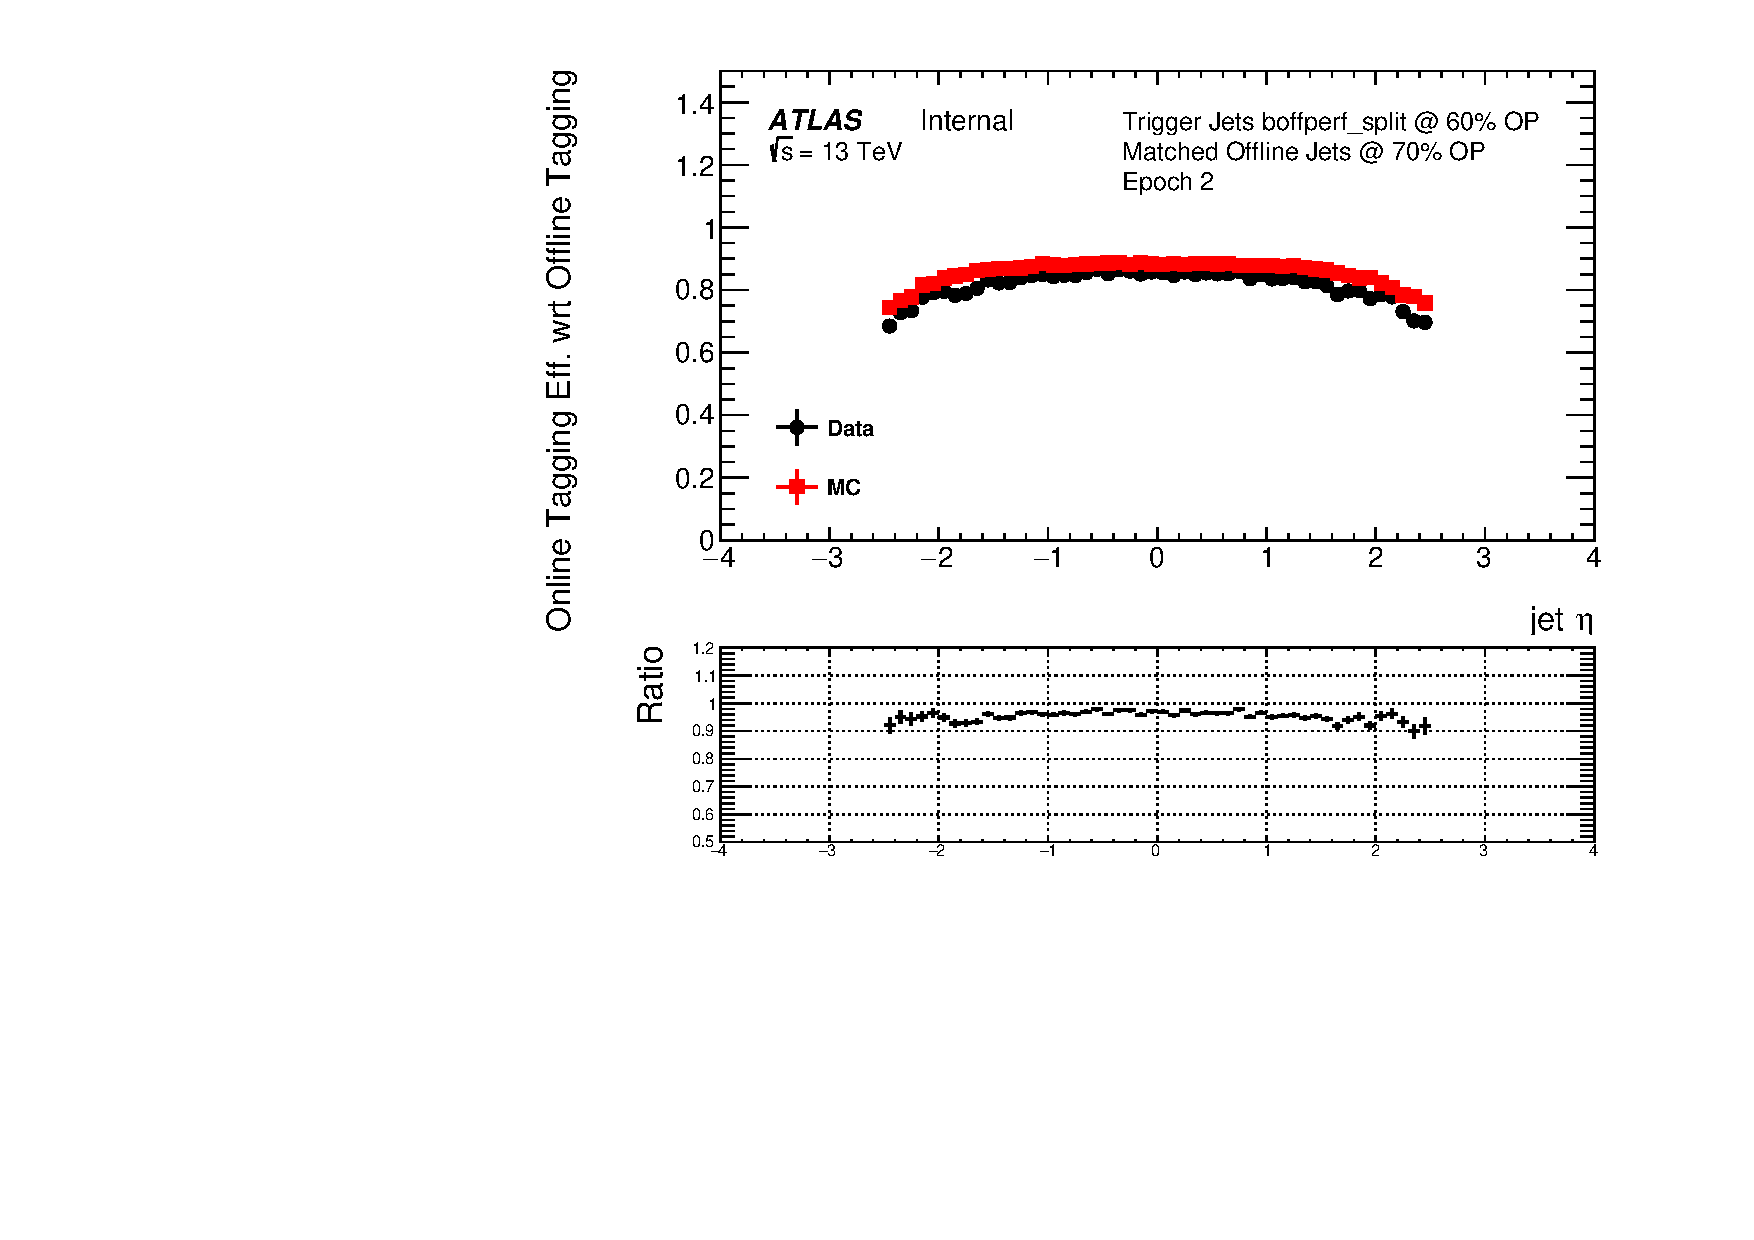
\includegraphics[width=0.47\linewidth, angle=0]{figs/Trigger/btrigger_old/Epoch2_trigReq_eff_jetEta.pdf}} \\
  %\subcaptionbox{??}{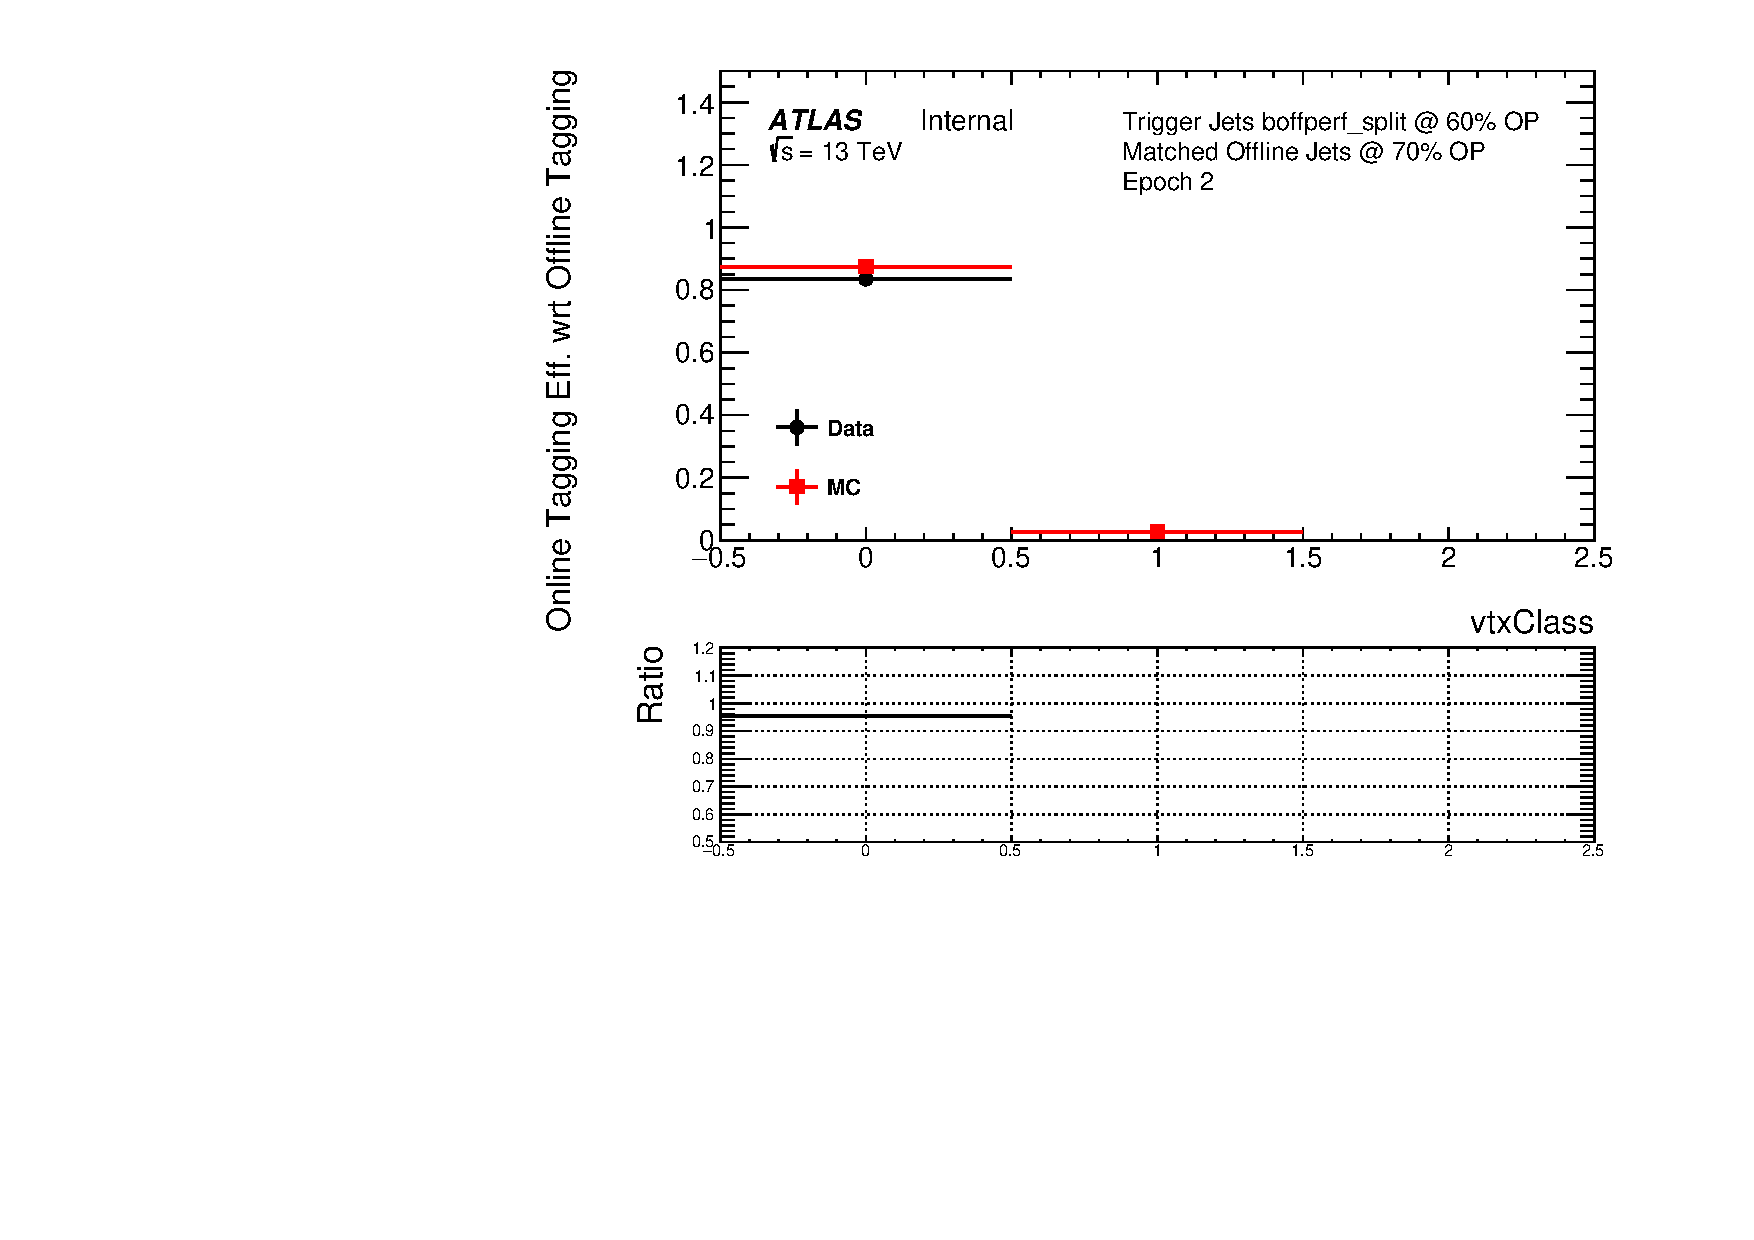
\includegraphics[width=0.47\linewidth, angle=0]{figs/Trigger/btrigger_old/Epoch2_trigReq_eff_vtxClass.pdf}}
\end{center}
\caption{The 60\% $b$-jet trigger efficiency with respect to an offline 70\% operating point tag
         for data from epoch 2 (black) and simulation (red) against jet-\pT~(a), jet-$\eta$ (b) and online beamspot $z$-position (c).}
\label{fig:Epoch2_eff}
\begin{center}
  \captionsetup[subfigure]{aboveskip=0pt,justification=centering}
  \subcaptionbox{Leading Jet-\pT}{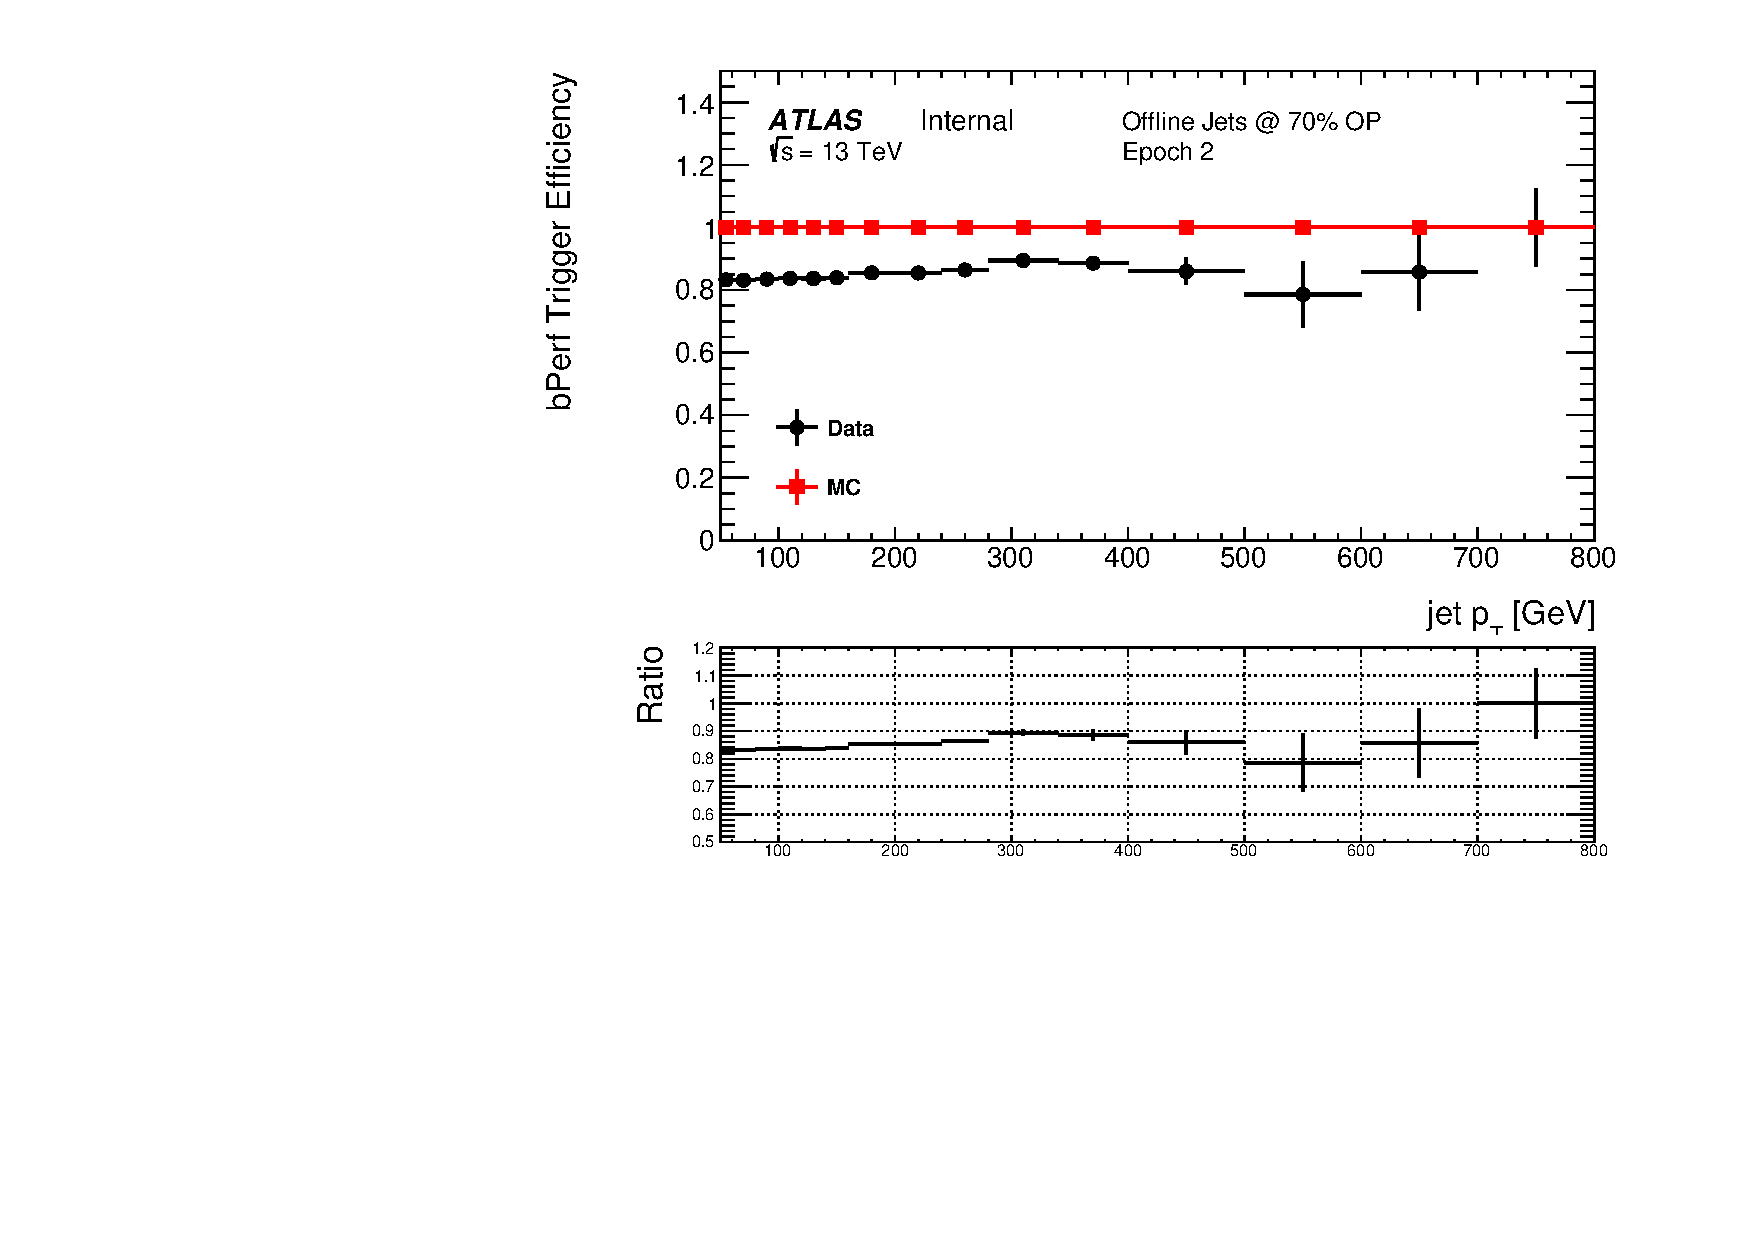
\includegraphics[width=0.47\linewidth, angle=0]{figs/Trigger/btrigger_old/Epoch2_trigReq_bPerfEff_jetPt.pdf}}
  \subcaptionbox{$z_{bs}^{online}$}{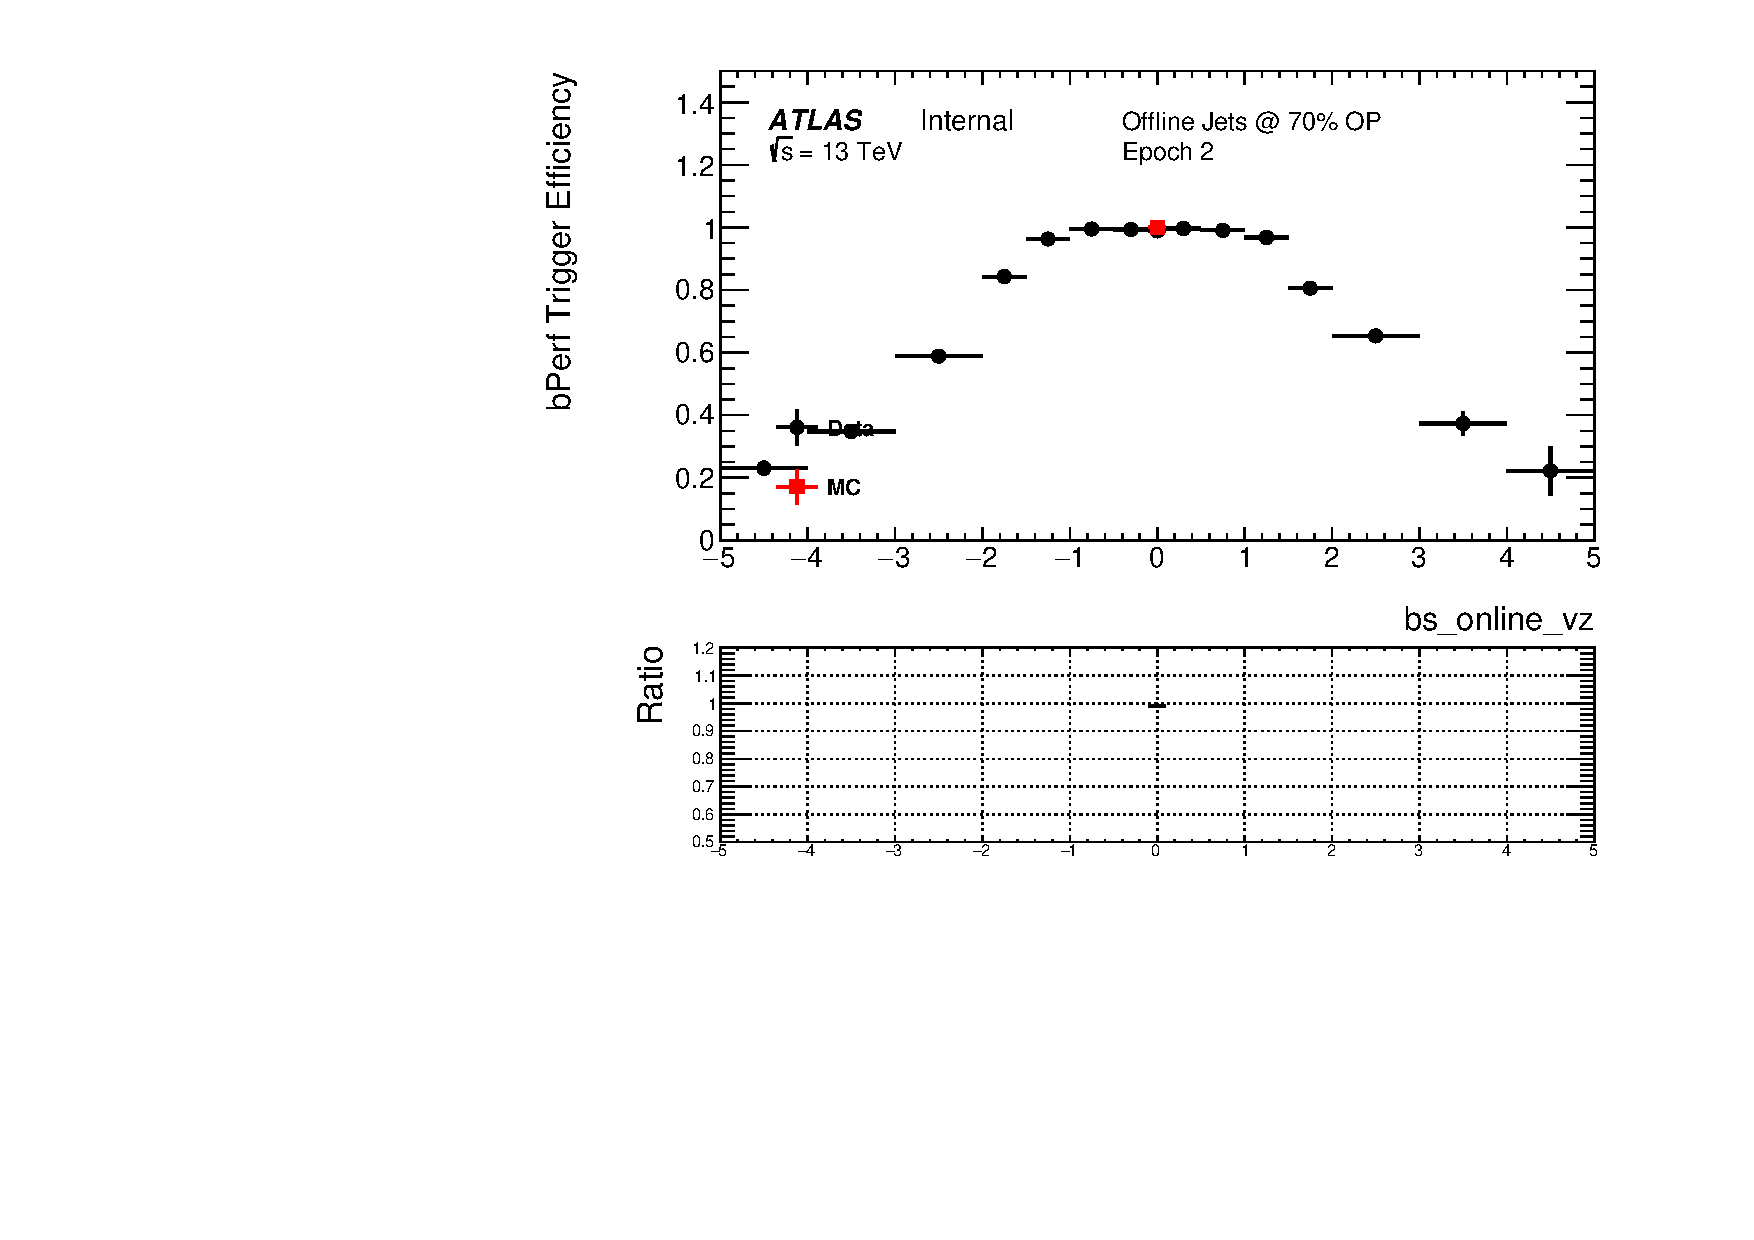
\includegraphics[width=0.47\linewidth, angle=0]{figs/Trigger/btrigger_old/Epoch2_trigReq_bPerfEff_bs_online_vz.pdf}}
  \subcaptionbox{Leading Jet-$\eta$}{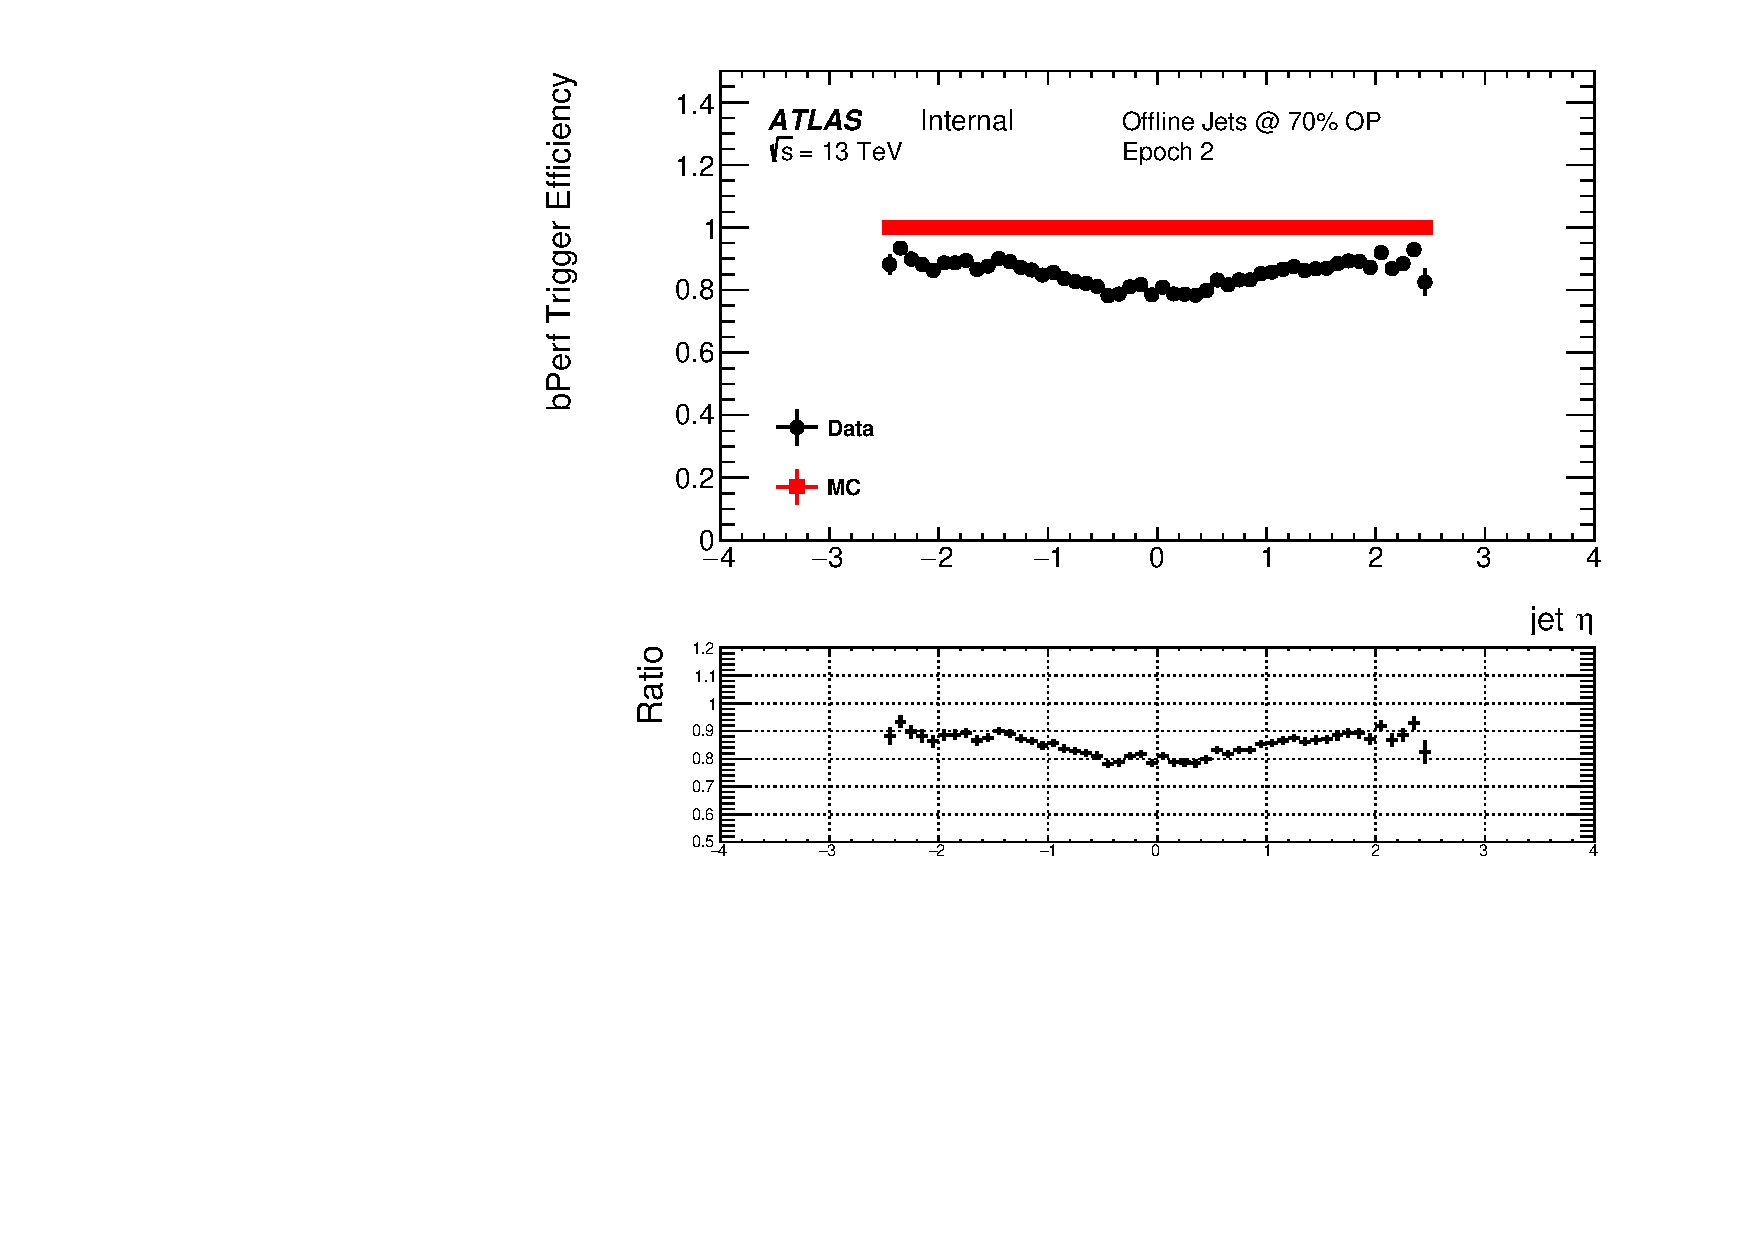
\includegraphics[width=0.47\linewidth, angle=0]{figs/Trigger/btrigger_old/Epoch2_trigReq_bPerfEff_jetEta.pdf}}
\end{center}
\caption{$b$-perf efficiency, $\epsilon_{bPerf}$, for data from Epoch 2 (black) and simulation (red) against leading-jet \pT~(a), online beamspot $z$-position (b) and leading jet-$\eta$ (c).}
\label{fig:Epoch2_bperf}
\end{figure}
Epoch 3, when no \verb|xPrmVtx| PV is found then a backup PV finding algorithm is used, known as \verb|EFHist|, which finds the PV through a basic histogramming of the tracks,
the simplicity of the algorithm means that a PV can be found as long as 1 track is present.
Figure~\ref{fig:Epoch3_eff} shows $\epsilon_{bTrig}$ for Epoch 3 for jet-\pT, jet-$\eta$,  $z_{bs}^{online}$ and vertex class (as defined above).
In Epoch 3 $\epsilon_{bTrig}$ measured in data is within 5\% of simulation and there is no shape difference between the two with respect to jet-$\eta$.
In addition it is shown that in Epoch 3 there is no strong dependence on  $z_{bs}^{online}$,
and that efficiency in data is consistent if a valid \verb|xPrmVtx| vertex or not (vertex class = 0 or 1 respectively).
This demonstrates the success of the backup vertex approach.

\begin{figure}[!ht]
\begin{center}
  \captionsetup[subfigure]{aboveskip=0pt,justification=centering}
  \subcaptionbox{Jet-\pT}{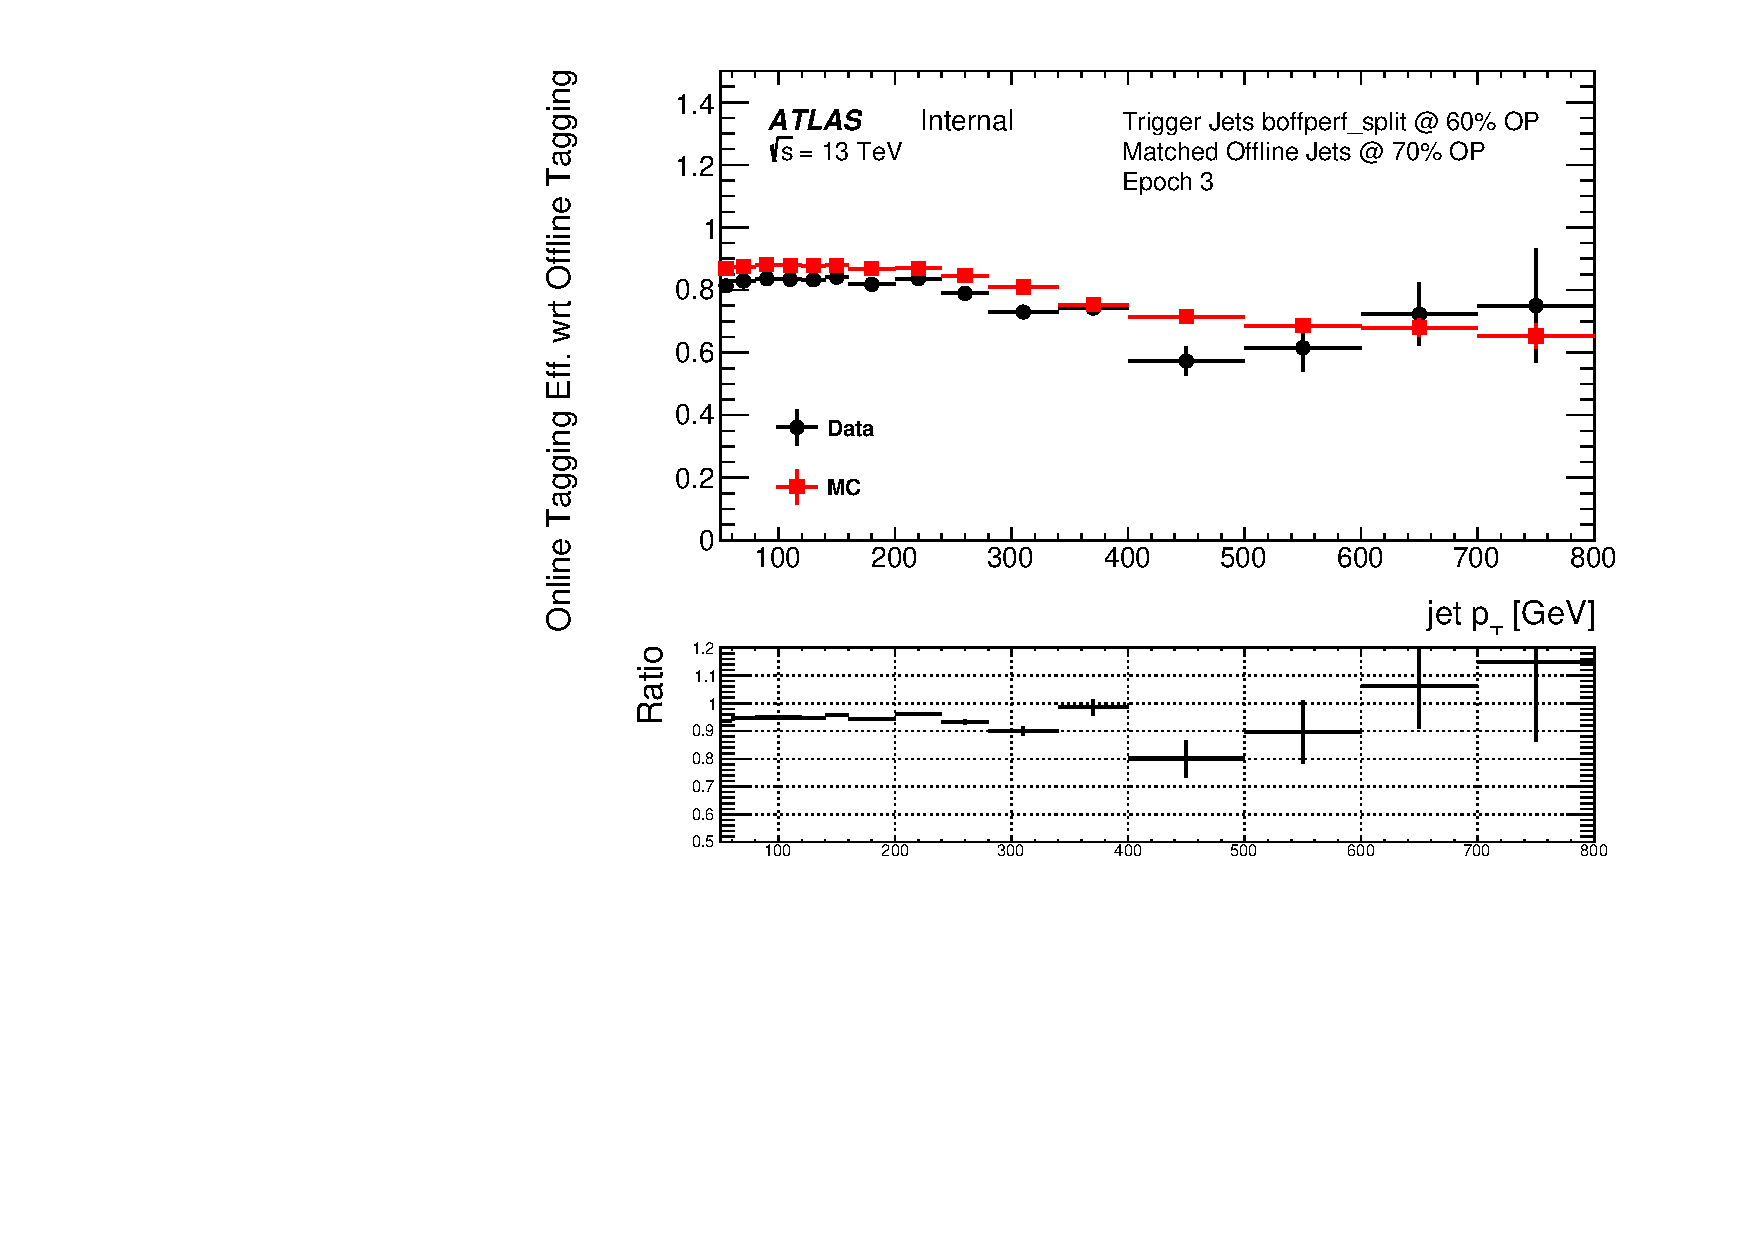
\includegraphics[width=0.47\linewidth, angle=0]{figs/Trigger/btrigger_old/Epoch3_trigReq_eff_jetPt.pdf}}
  \subcaptionbox{Jet-$\eta$}{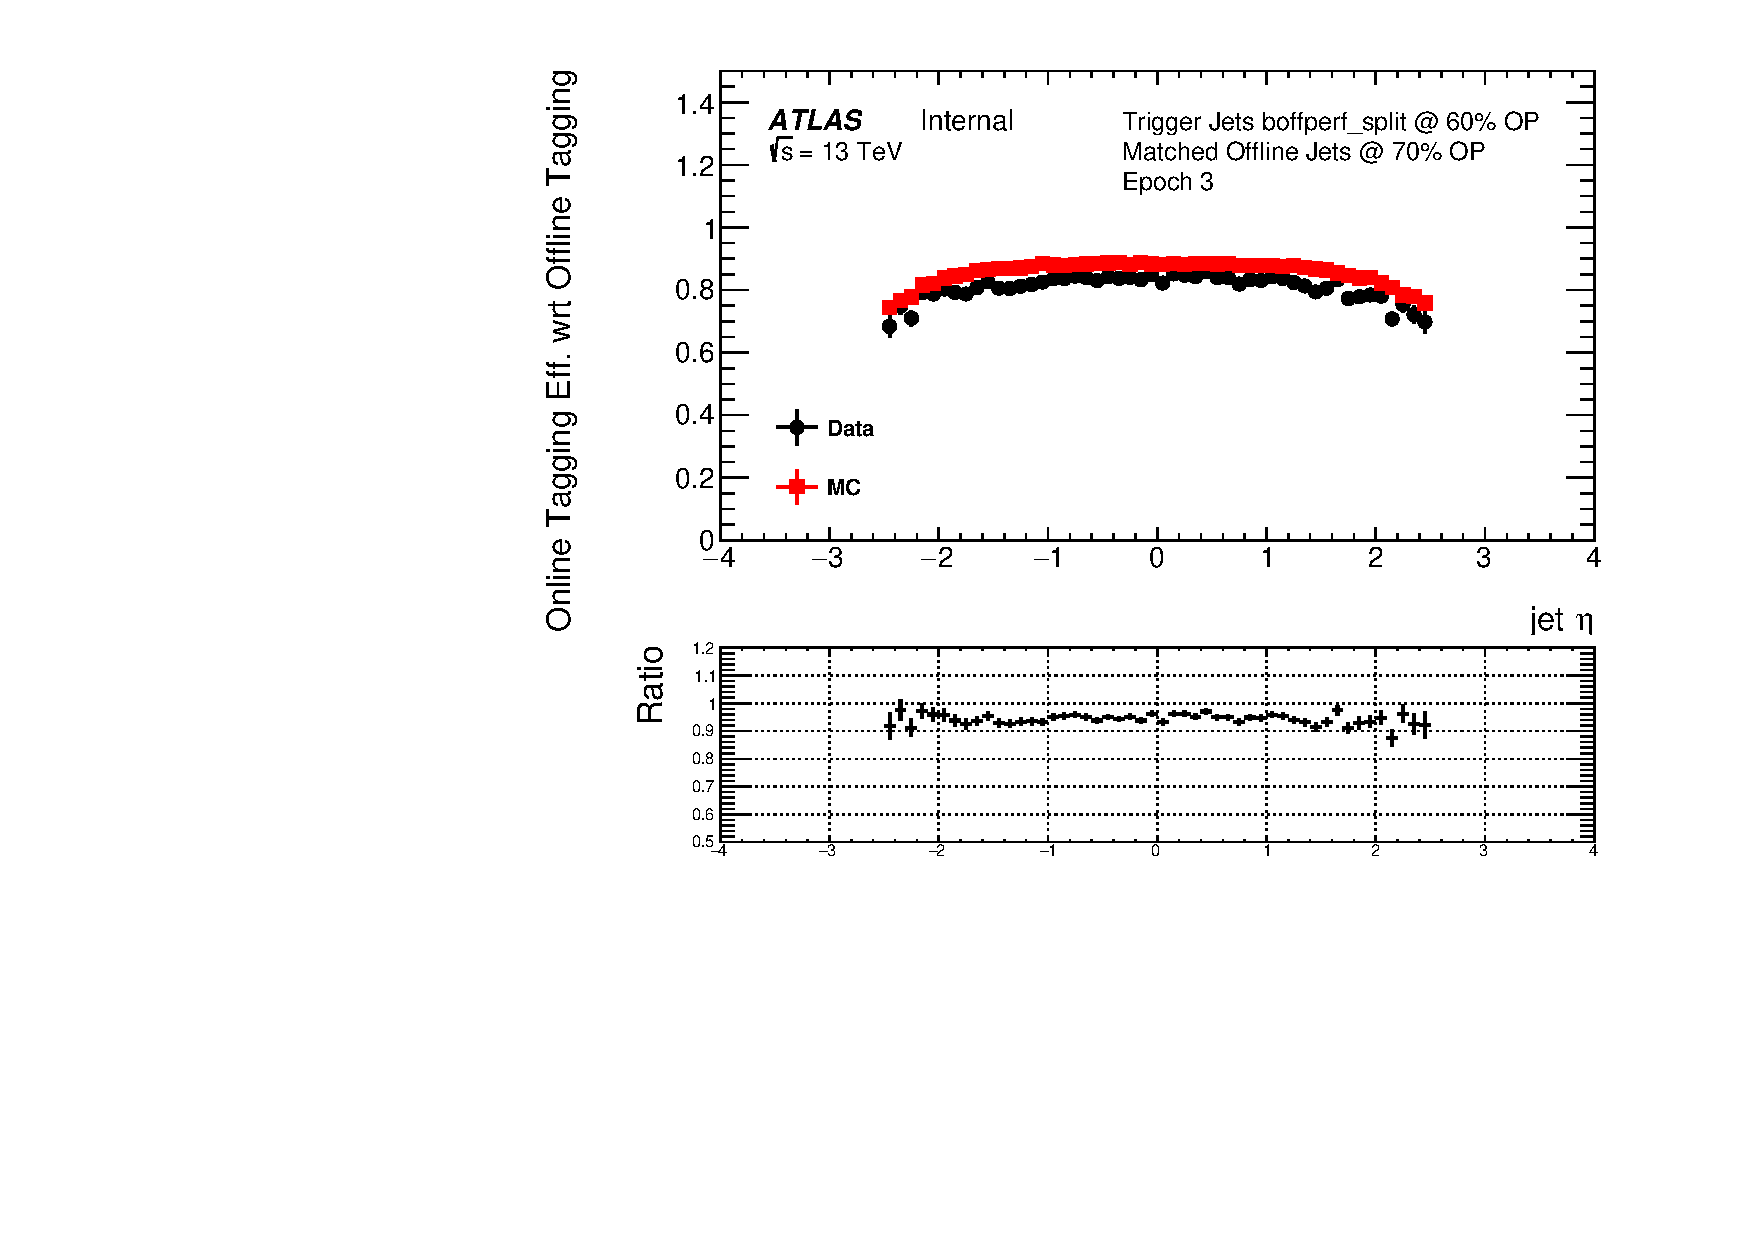
\includegraphics[width=0.47\linewidth, angle=0]{figs/Trigger/btrigger_old/Epoch3_trigReq_eff_jetEta.pdf}} \\
  \subcaptionbox{$z_{bs}^{online}$}{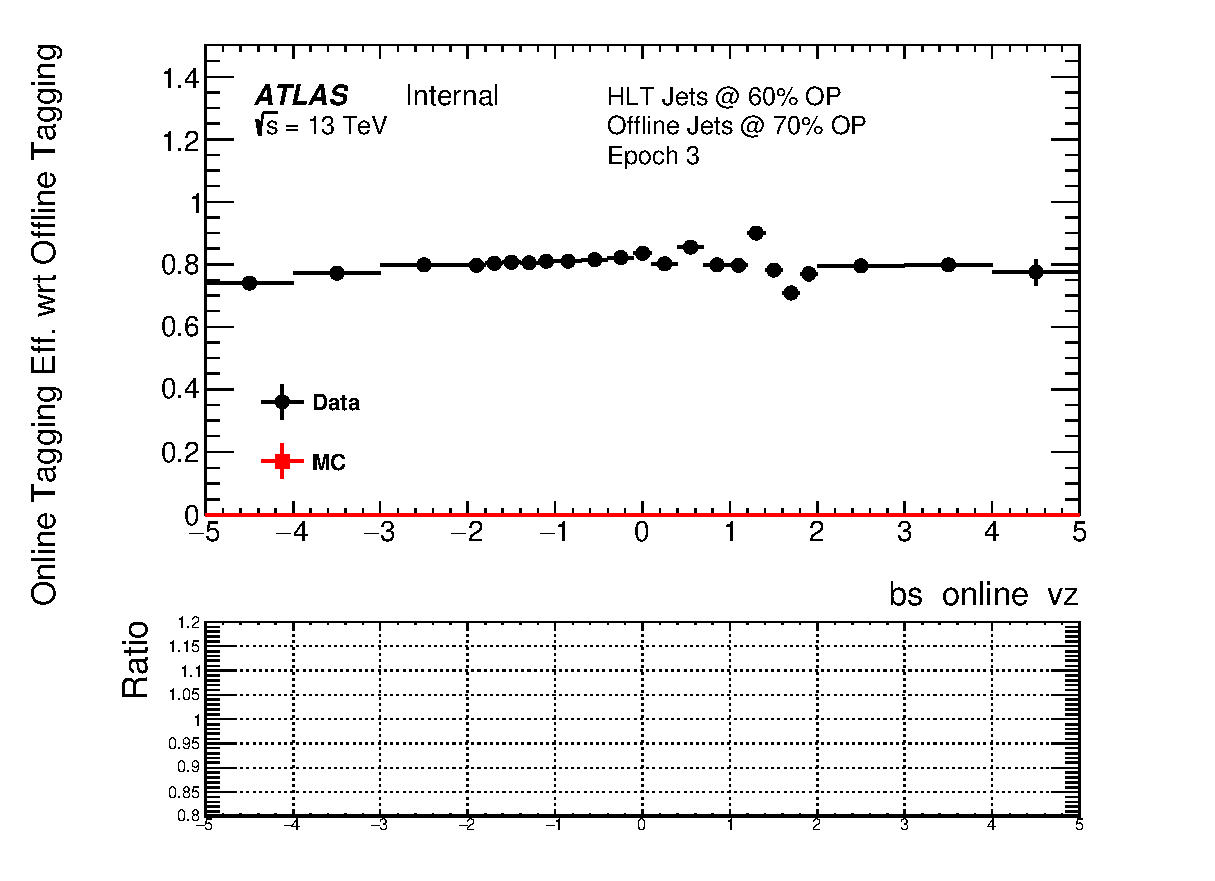
\includegraphics[width=0.47\linewidth, angle=0]{figs/Trigger/Epoch3_eff_bs_online_vz.eps}}
  \subcaptionbox{Vertex Class}{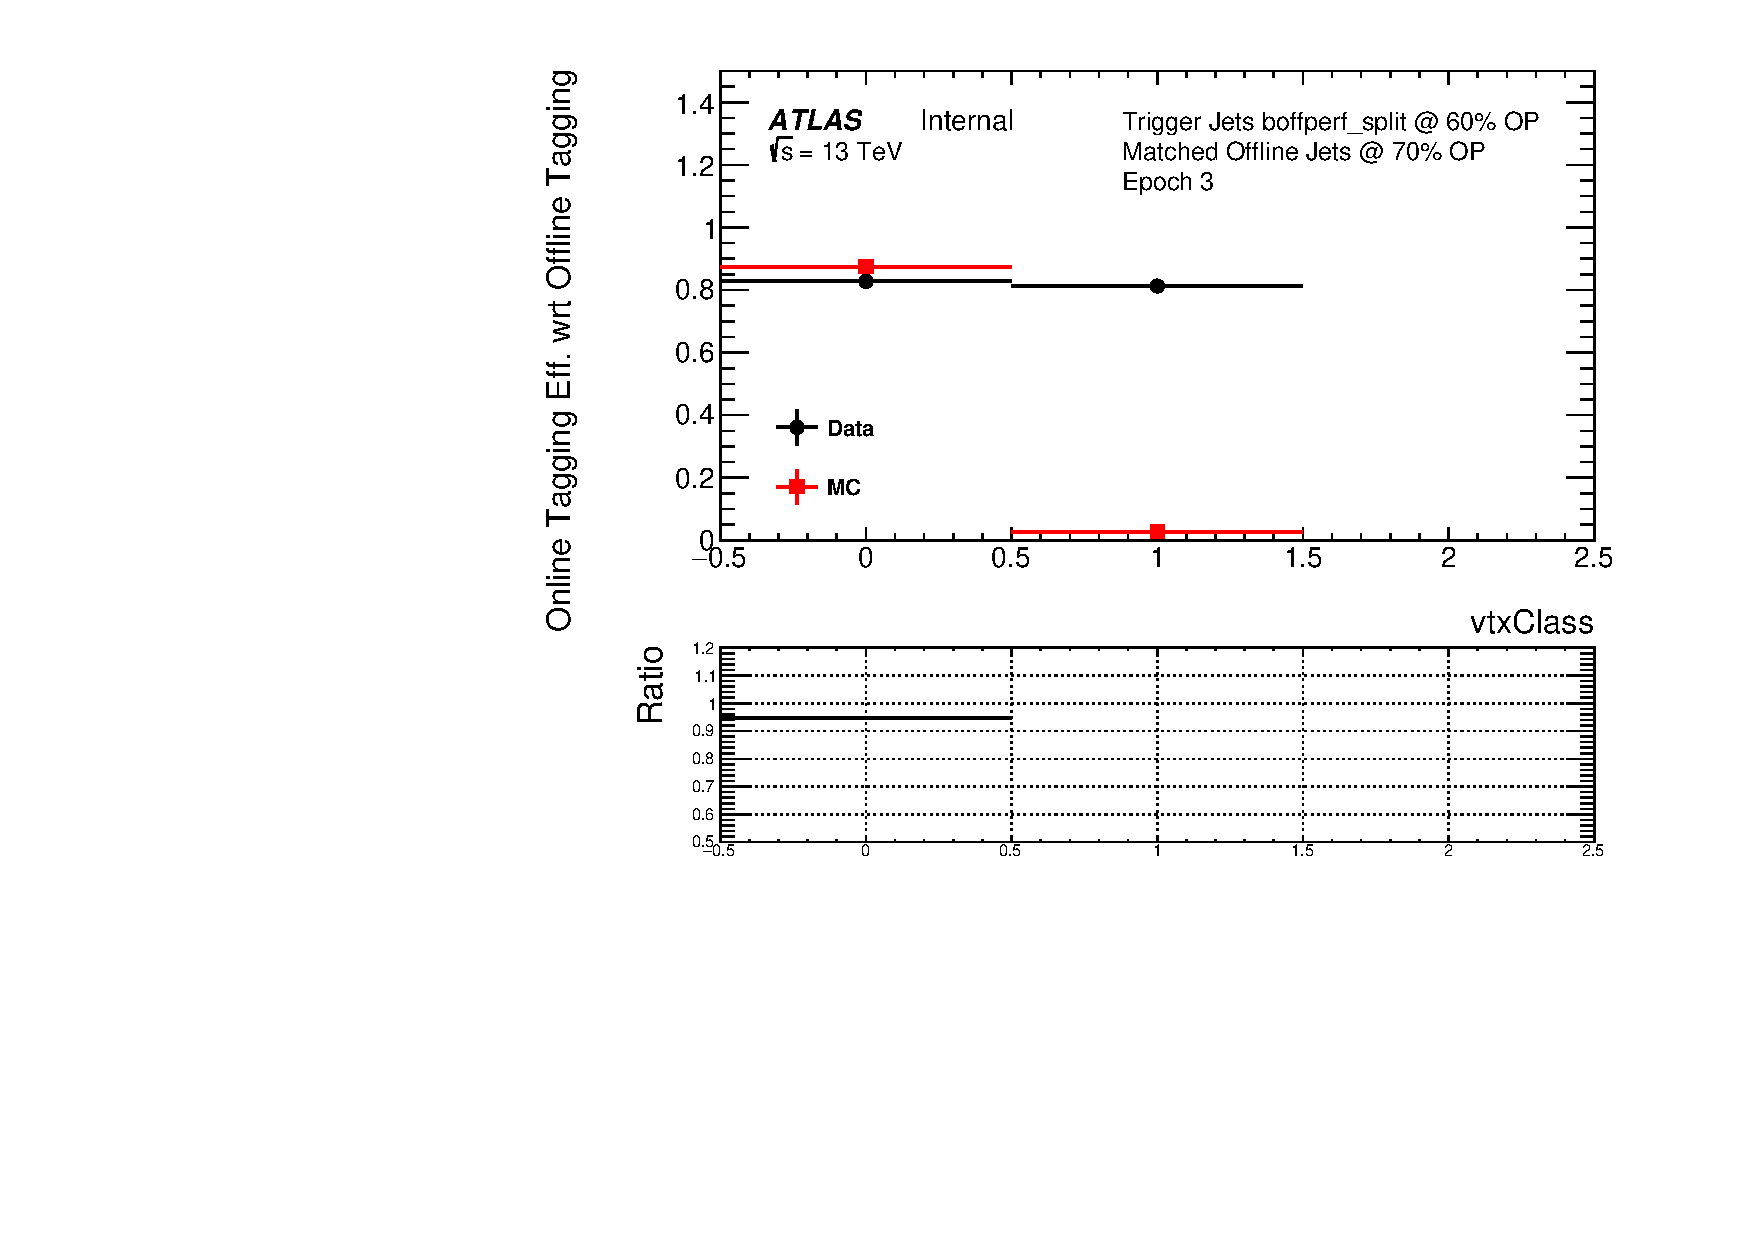
\includegraphics[width=0.47\linewidth, angle=0]{figs/Trigger/btrigger_old/Epoch3_trigReq_eff_vtxClass.pdf}}
\end{center}
\caption{The 60\% $b$-jet trigger efficiency with respect to an offline 70\% operating point tag
  for data from Epoch 3 (black) and simulation (red) against (a) jet-\pT, (b) jet-$\eta$,
  (c) online beamspot $z$-position and (d) vertex class.}
\label{fig:Epoch3_eff}
\end{figure}

\FloatBarrier

\subsection{Solution: $b$-Jet Trigger GRL}
\label{sec:trig-inv}

To summarise, in the previous section it is shown that at large values of absolute online beamspot $z$-position
the measured $\epsilon_{bTrig}$ in Epoch 1 and $\epsilon_{bPerf}$ in Epoch 2 is lower in data than in MC, due to poor \verb|xPrmVtx| PV finding performance.
In Epoch 3 there is reasonable data/simulation agreement due to the use of a backup vertex finding algorithm. 

The solution employed is to apply a $b$-jet trigger aware GRL 
that removes events with an absolute  $z_{bs}^{online}$ greater than 2mm in Epoch 1 and 2,
such that the events with low efficiency are removed.
The cost of this approach is the luminosity of our data-set is reduced, specifically the data-set falls from  32.9~\ifb to 24.3~\ifb.
However there are three key reasons why use of a $b$-jet trigger GRL was chosen over simply applying an overall efficiency.
Firstly, as there is no beamspot position distribution in simulation it is not clear that kinematics of events at high  $z_{bs}^{online}$ can be well understood and modelled;
the sculpting of the efficiency with respect to jet-$\eta$ is an example of this.
Secondly, the efficiencies are quite low at high beamspot $z$-position,
so the loss in luminosity x acceptance is relatively small
and finally the use of a GRL means a more realistic estimate of the actual luminosity used in an analysis is used. 

For the choice of which value of beamspot $z$ position to use for in the GRL,
it was required to select the widest cut where the efficiency had not significantly declined,
such that as much luminosity as possible is retained while removing most of the affected region.
This \SI{2}{\mm} cut was chosen from examining Figure~\ref{fig:Epoch1_eff}(b) and Figure~\ref{fig:Epoch2_bperf}(b)
and from studying a variety of cuts from \SI{2}{\mm} to \SI{1}{\mm}.

After the GRL is applied, $\epsilon_{bTrig}$ for Region 1 becomes approximately 90-95\% of the efficiency measured in simulation,
as shown in Figure~\ref{fig:Epoch1_bslt2mm_eff},
and $\epsilon_{bPerf}$ for Region 2 becomes approximately 95\% of the efficiency measured in simulation,
as shown in Figure~\ref{fig:Epoch2_bslt2mm_bperf}. 

\begin{figure}[!ht]
  \begin{center}
    \captionsetup[subfigure]{aboveskip=0pt,justification=centering}
    \subcaptionbox{Jet-\pT}{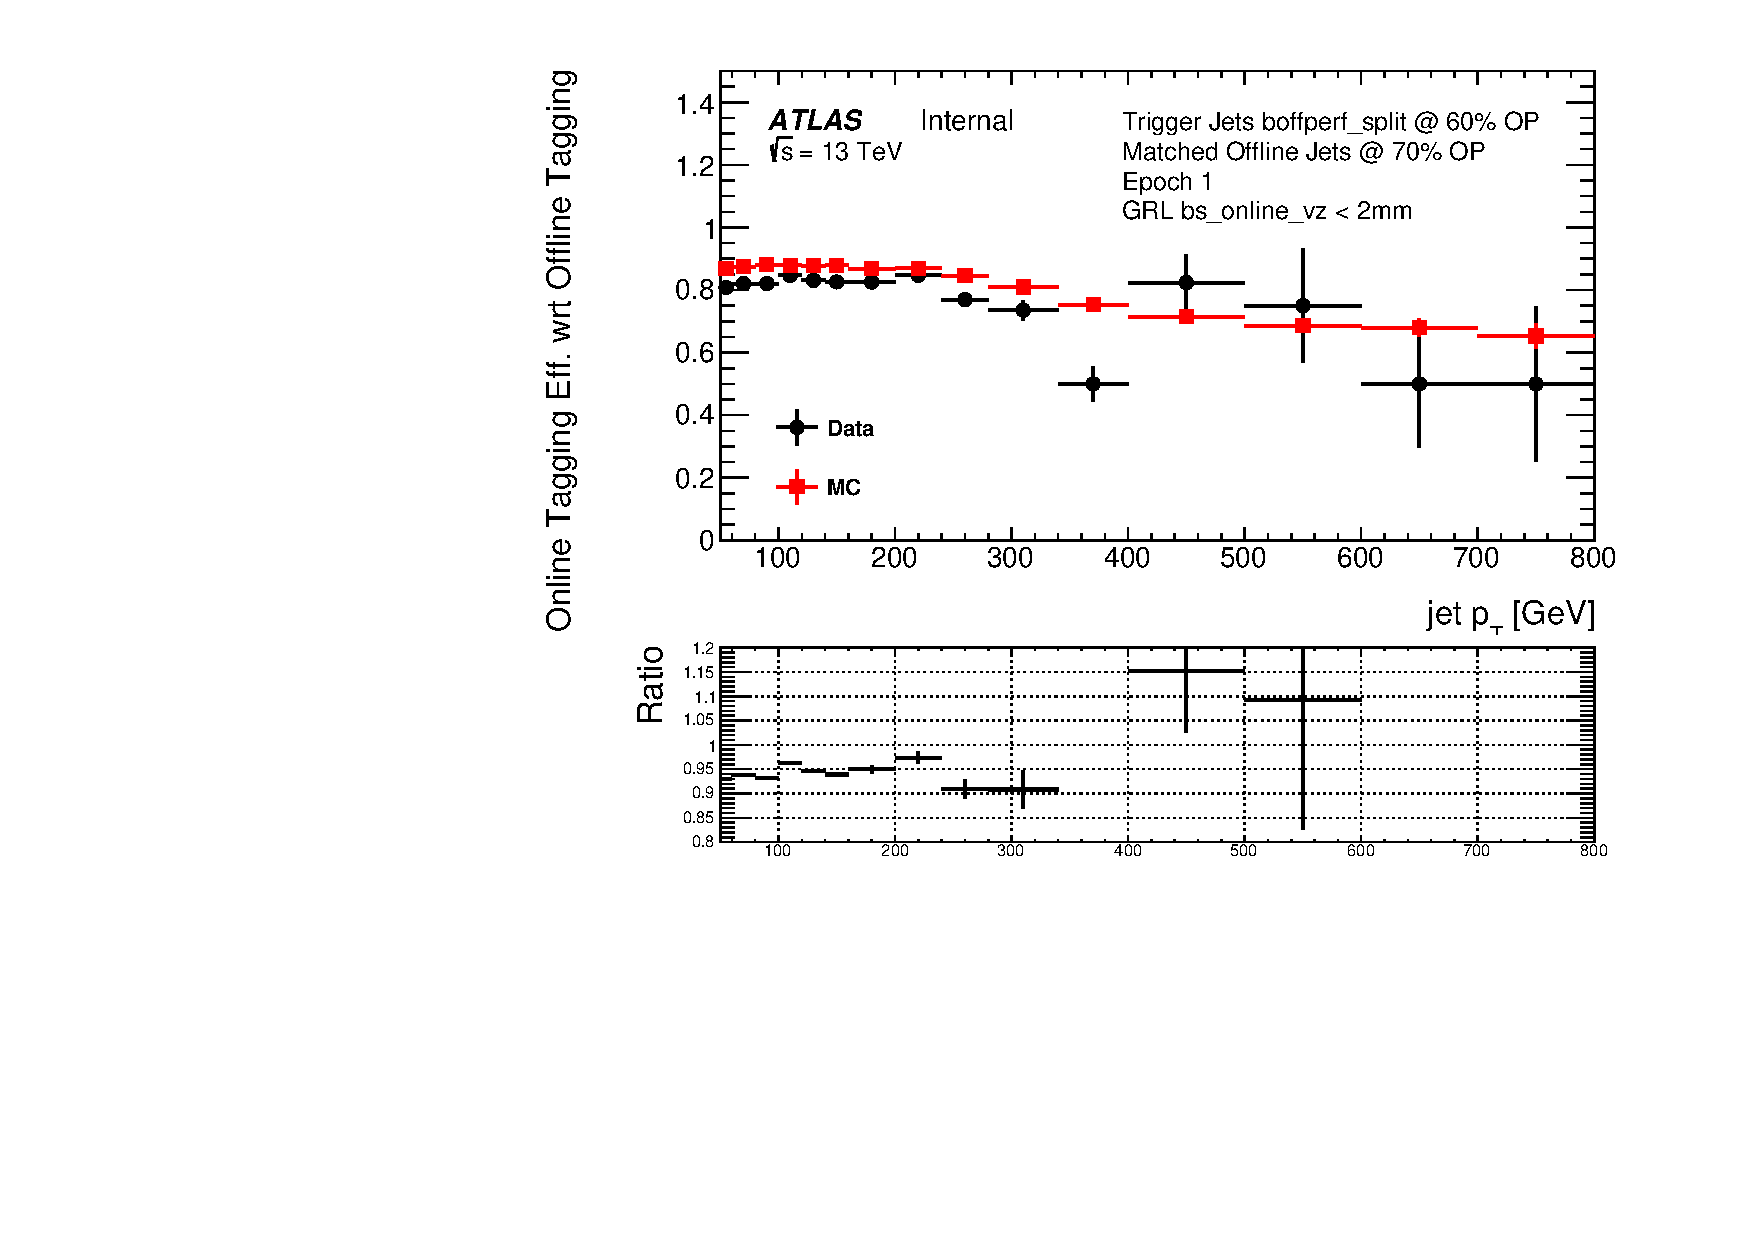
\includegraphics[width=0.47\linewidth, angle=0]{figs/Trigger/btrigger_old/Epoch1_GRL_bslt2mm_trigReq_eff_jetPt.pdf} }
    \subcaptionbox{Jet-$\eta$}{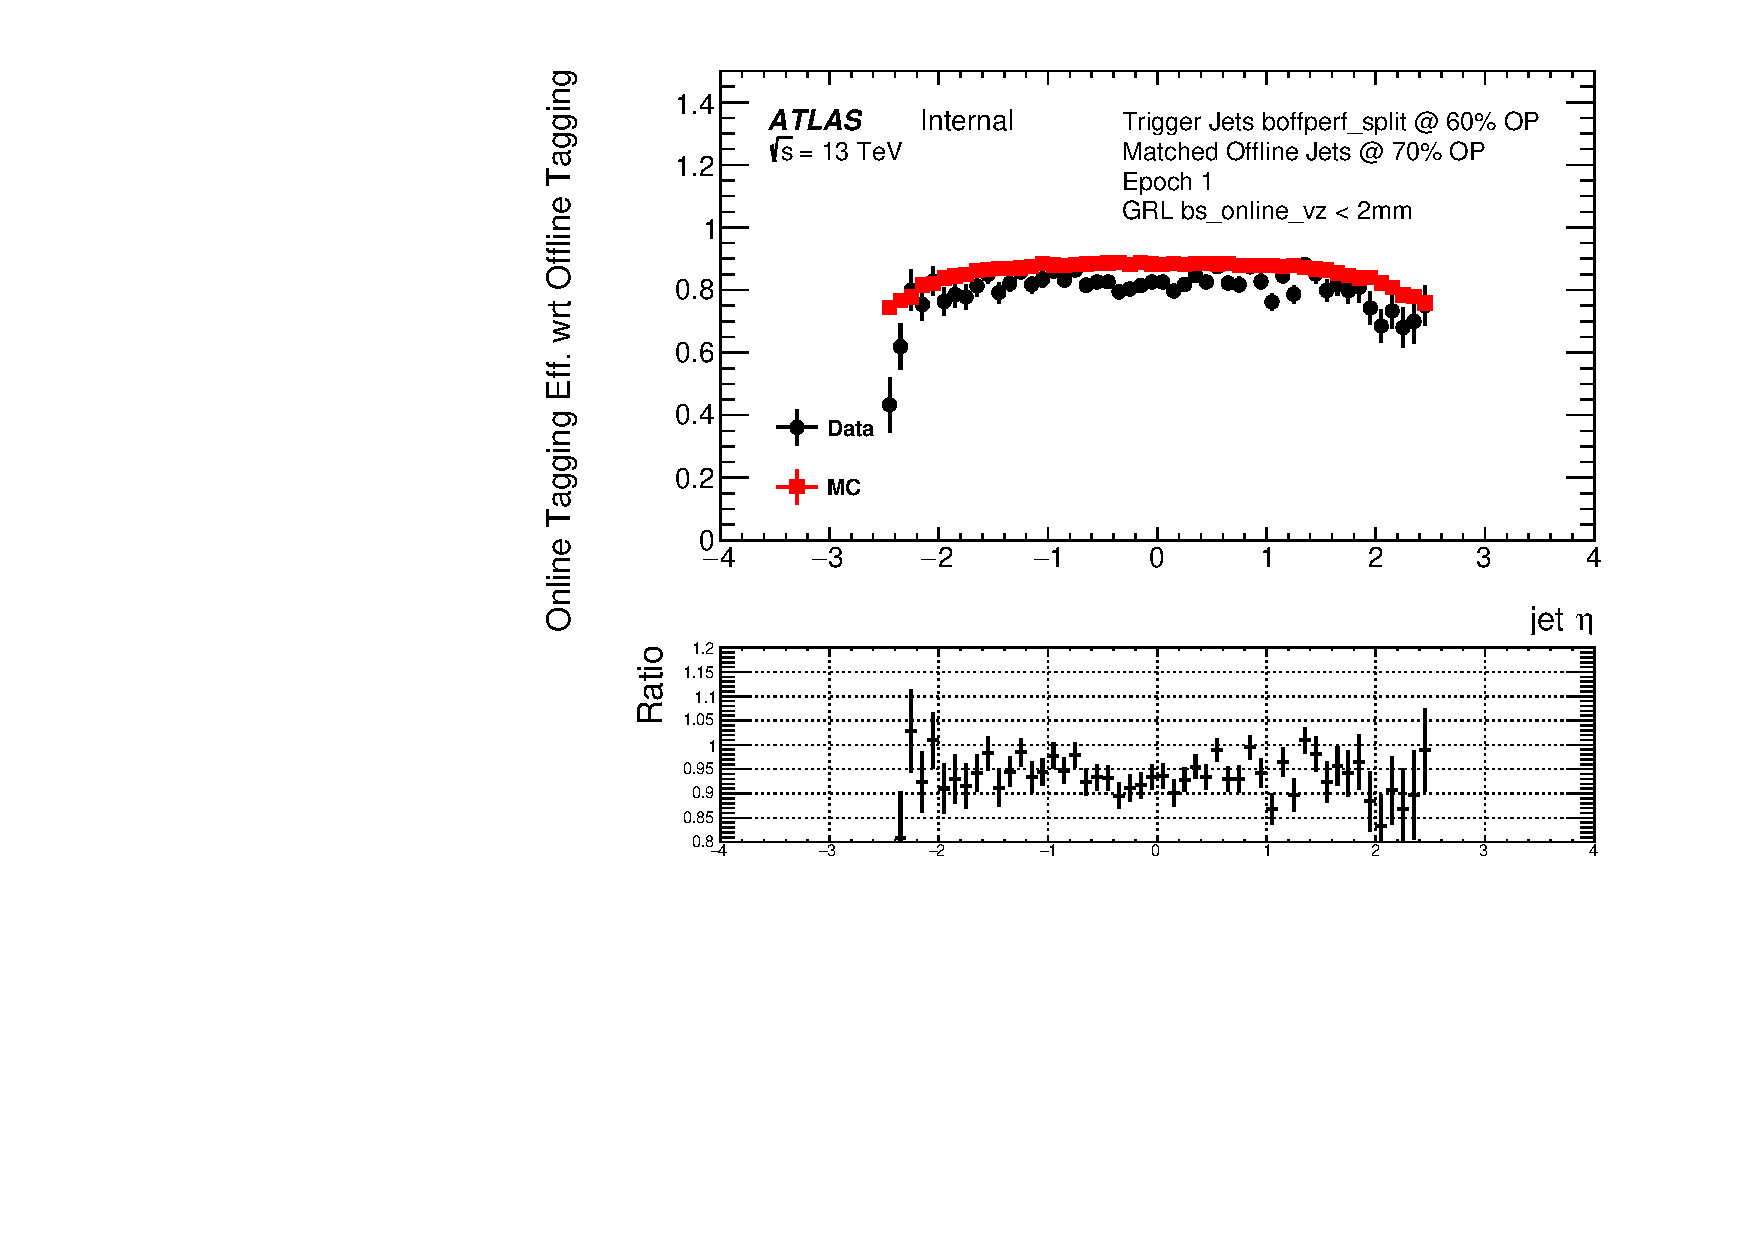
\includegraphics[width=0.47\linewidth, angle=0]{figs/Trigger/btrigger_old/Epoch1_GRL_bslt2mm_trigReq_eff_jetEta.pdf}}
  \end{center}
  \caption{The 60\% $b$-jet trigger efficiency with respect to an offline 70\% operating point tag
    for data from Region 1 (black) and simulation (red) against jet-\pT~(a) and jet-$\eta$ (b).
    The $b$-jet trigger aware GRL has been applied.}
  \label{fig:Epoch1_bslt2mm_eff}
  \begin{center}
    \captionsetup[subfigure]{aboveskip=0pt,justification=centering}
    \subcaptionbox{Leading Jet-\pT}{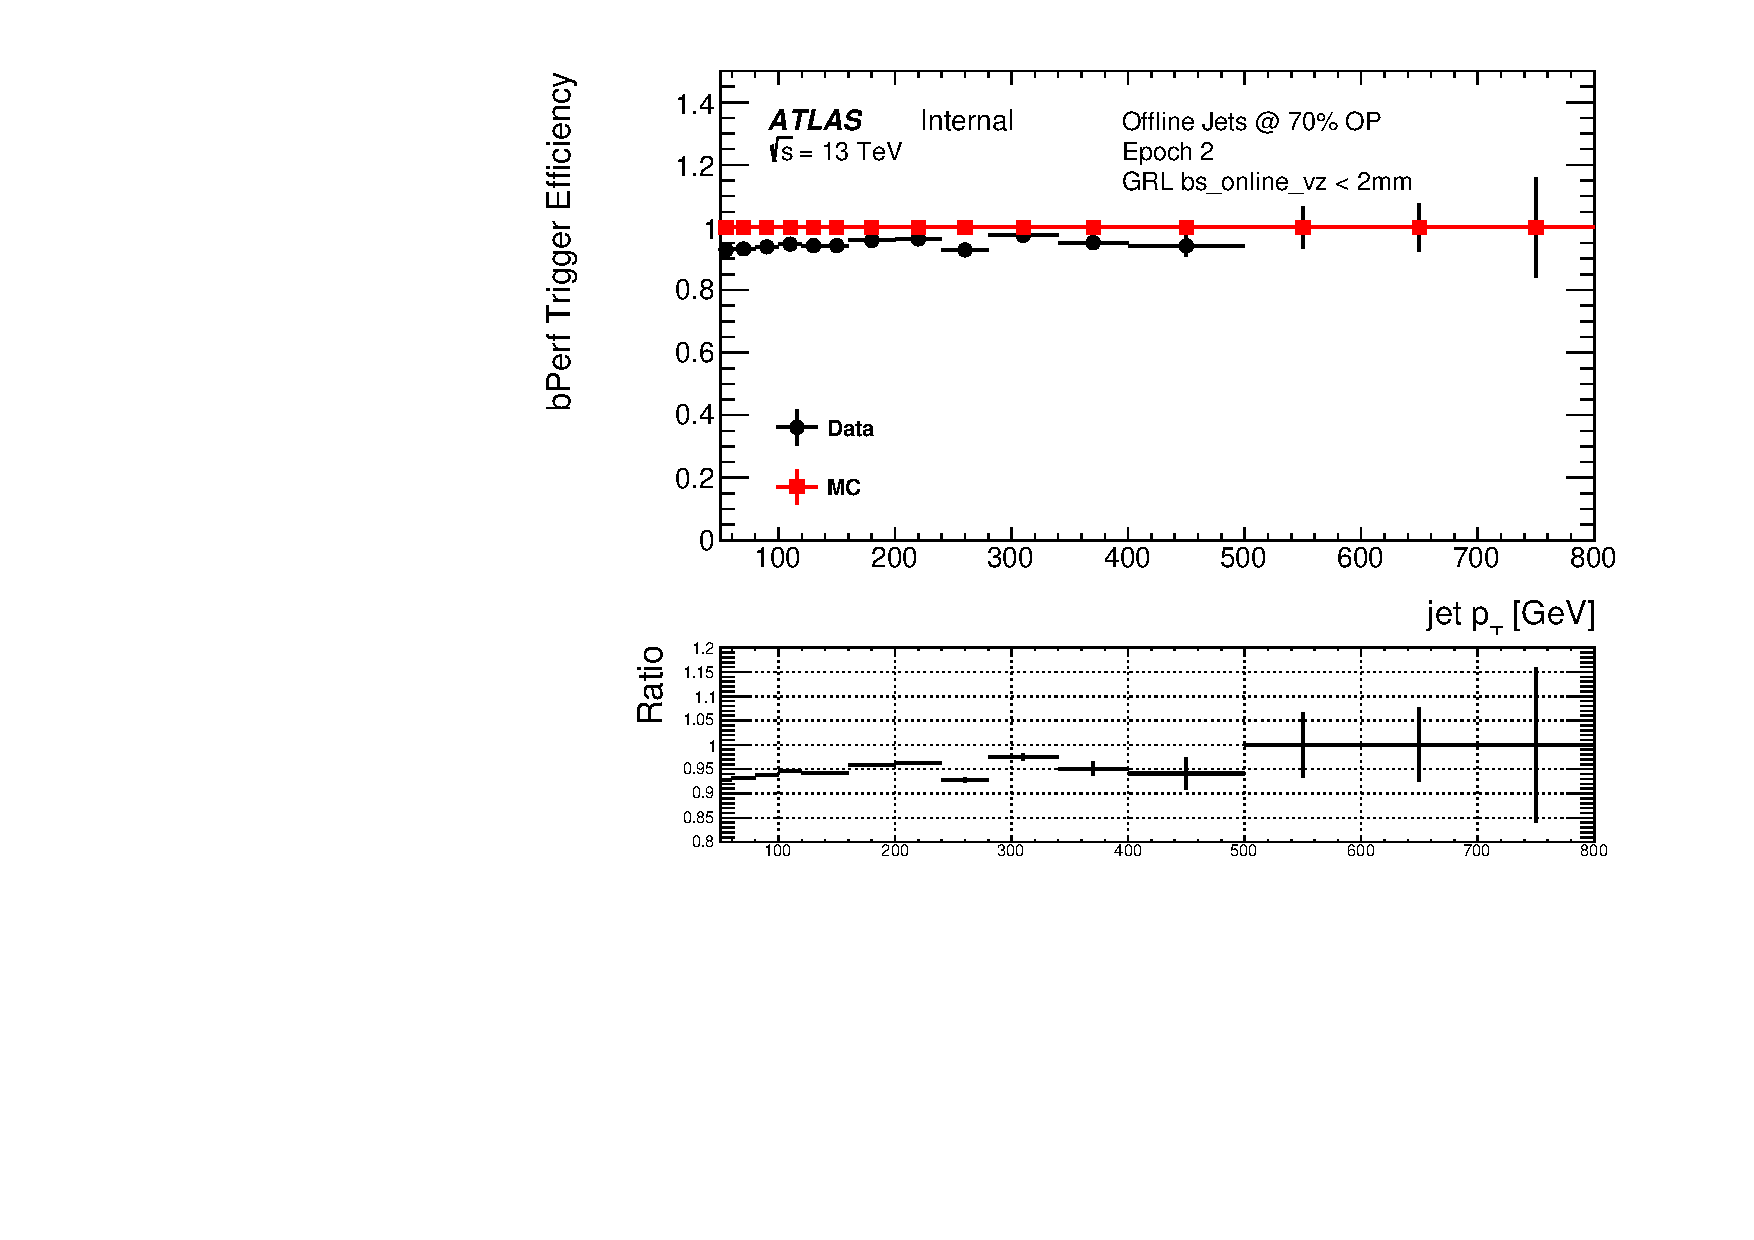
\includegraphics[width=0.47\linewidth, angle=0]{figs/Trigger/btrigger_old/Epoch2_GRL_bslt2mm_trigReq_bPerfEff_jetPt.pdf} }
    \subcaptionbox{Leading Jet-$\eta$}{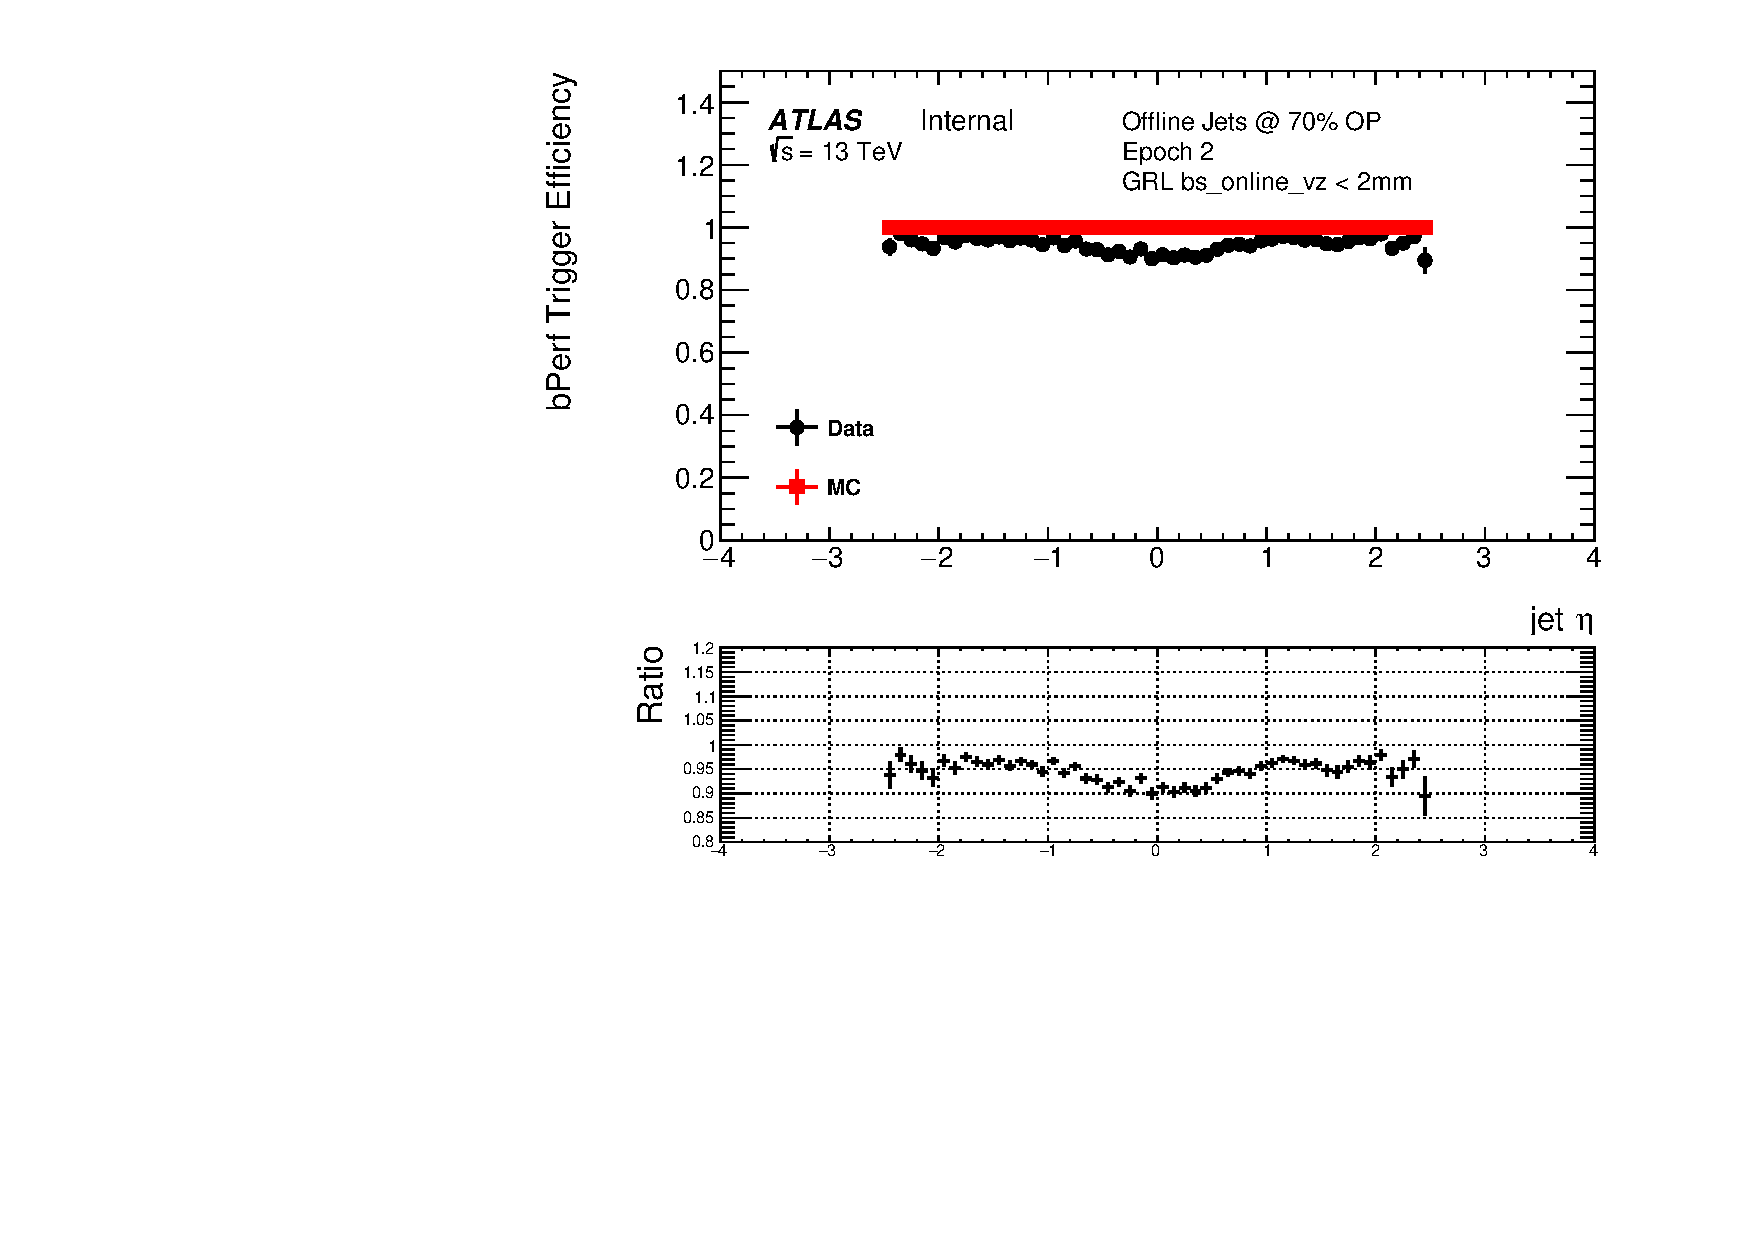
\includegraphics[width=0.47\linewidth, angle=0]{figs/Trigger/btrigger_old/Epoch2_GRL_bslt2mm_trigReq_bPerfEff_jetEta.pdf}}
  \end{center}
  \caption{$b$-perf efficiency, $\epsilon_{bPerf}$, for data from Region 2 (black) and simulation (red) against leading (a) jet-\pT~and (b) jet-$\eta$.
    The $b$-jet trigger aware GRL has been applied.}
  \label{fig:Epoch2_bslt2mm_bperf}
\end{figure}

\newpage

Figures~\ref{fig:Full_bslt2mm_eff} and ~\ref{fig:Full_bslt2mm_bperf}  shows measured
$\epsilon_{bPerf}$ and $\epsilon_{bTrig}$
for the full 2016 data-set, combining Regions 1, 2 and 3,
with the $b$-jet trigger aware GRL applied.
This represents the raw observed data/simulation efficiencies when the full event selection has been applied.

\begin{figure}[!ht]
  \begin{center}
    \captionsetup[subfigure]{aboveskip=0pt,justification=centering}
    \subcaptionbox{Jet-\pT}{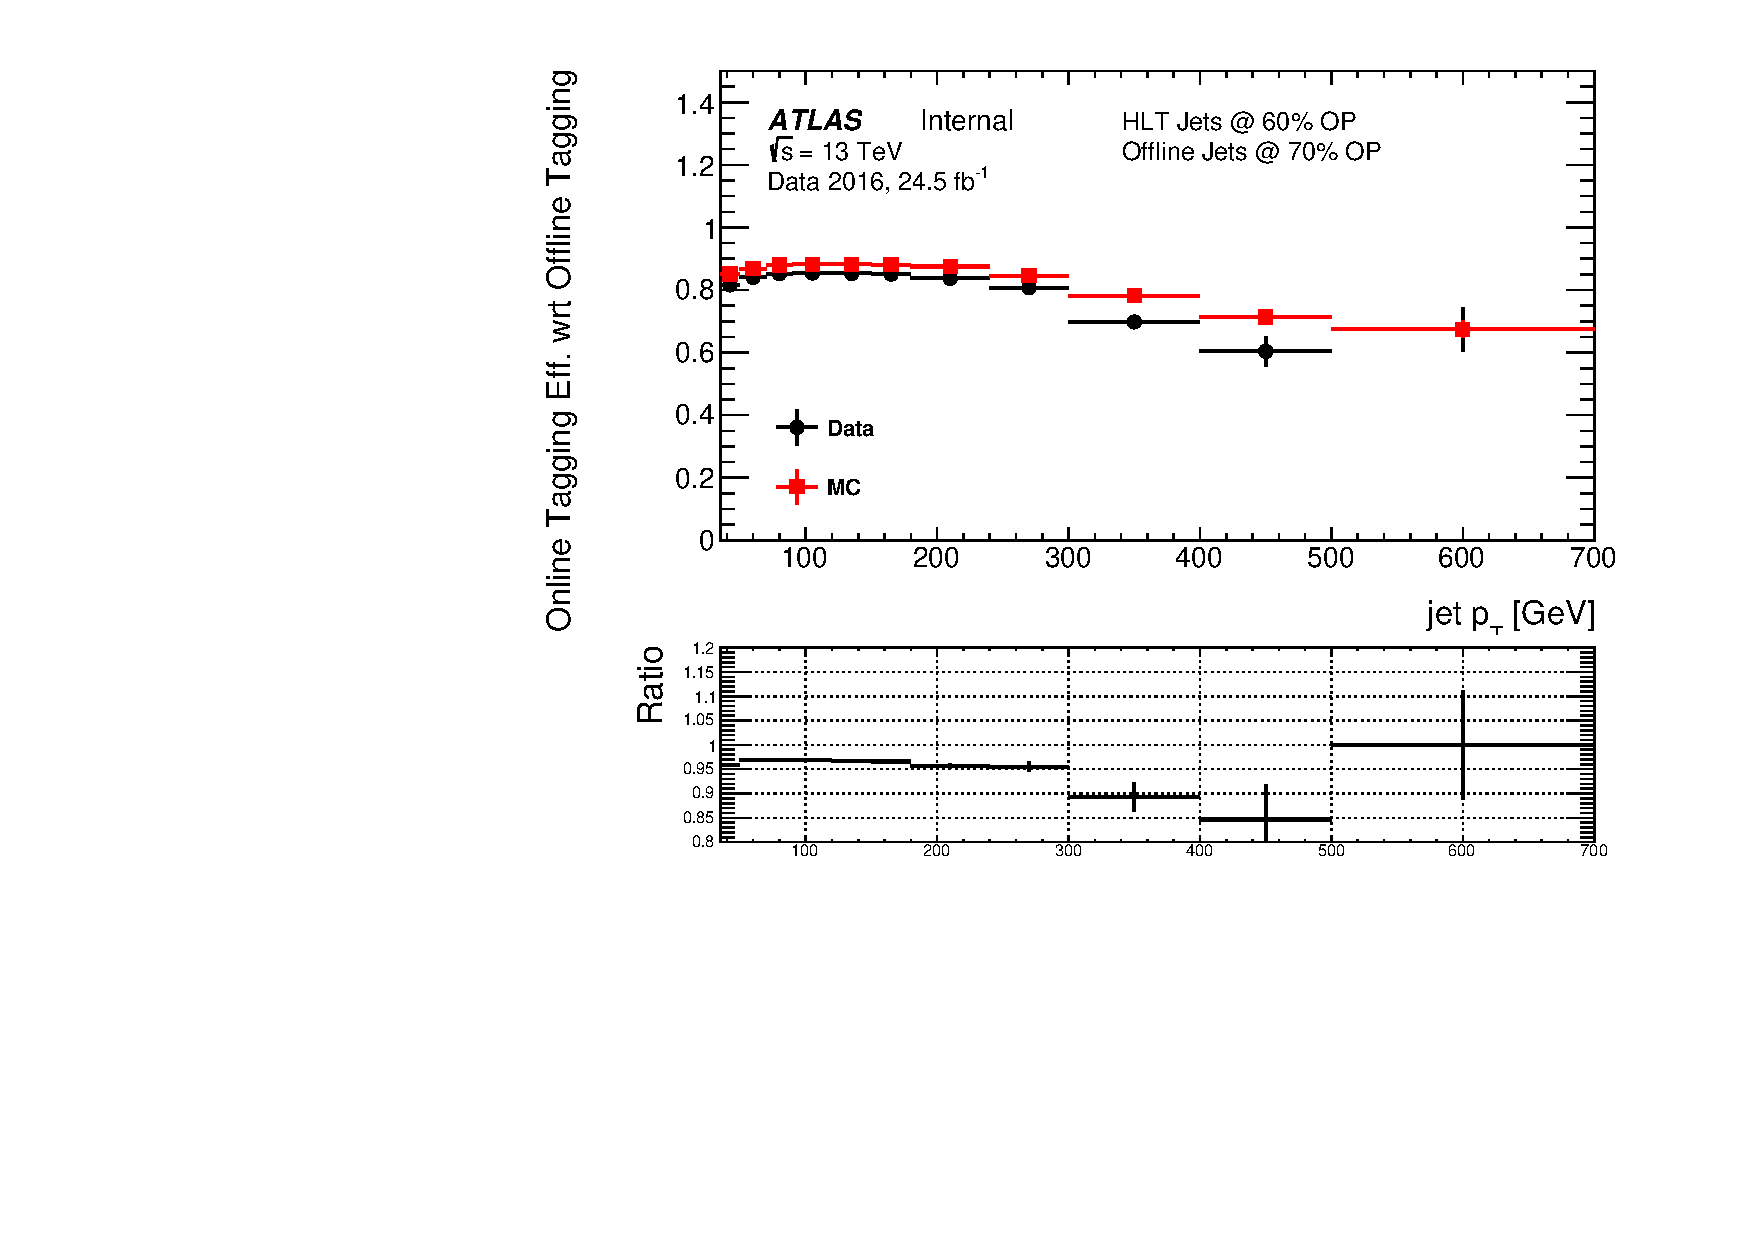
\includegraphics[width=0.47\linewidth, angle=0]{figs/Trigger/btrigger_old/Full_GRL_bslt2mm_trigReq_eff_jetPt.pdf}}
    \subcaptionbox{Jet-$\eta$}{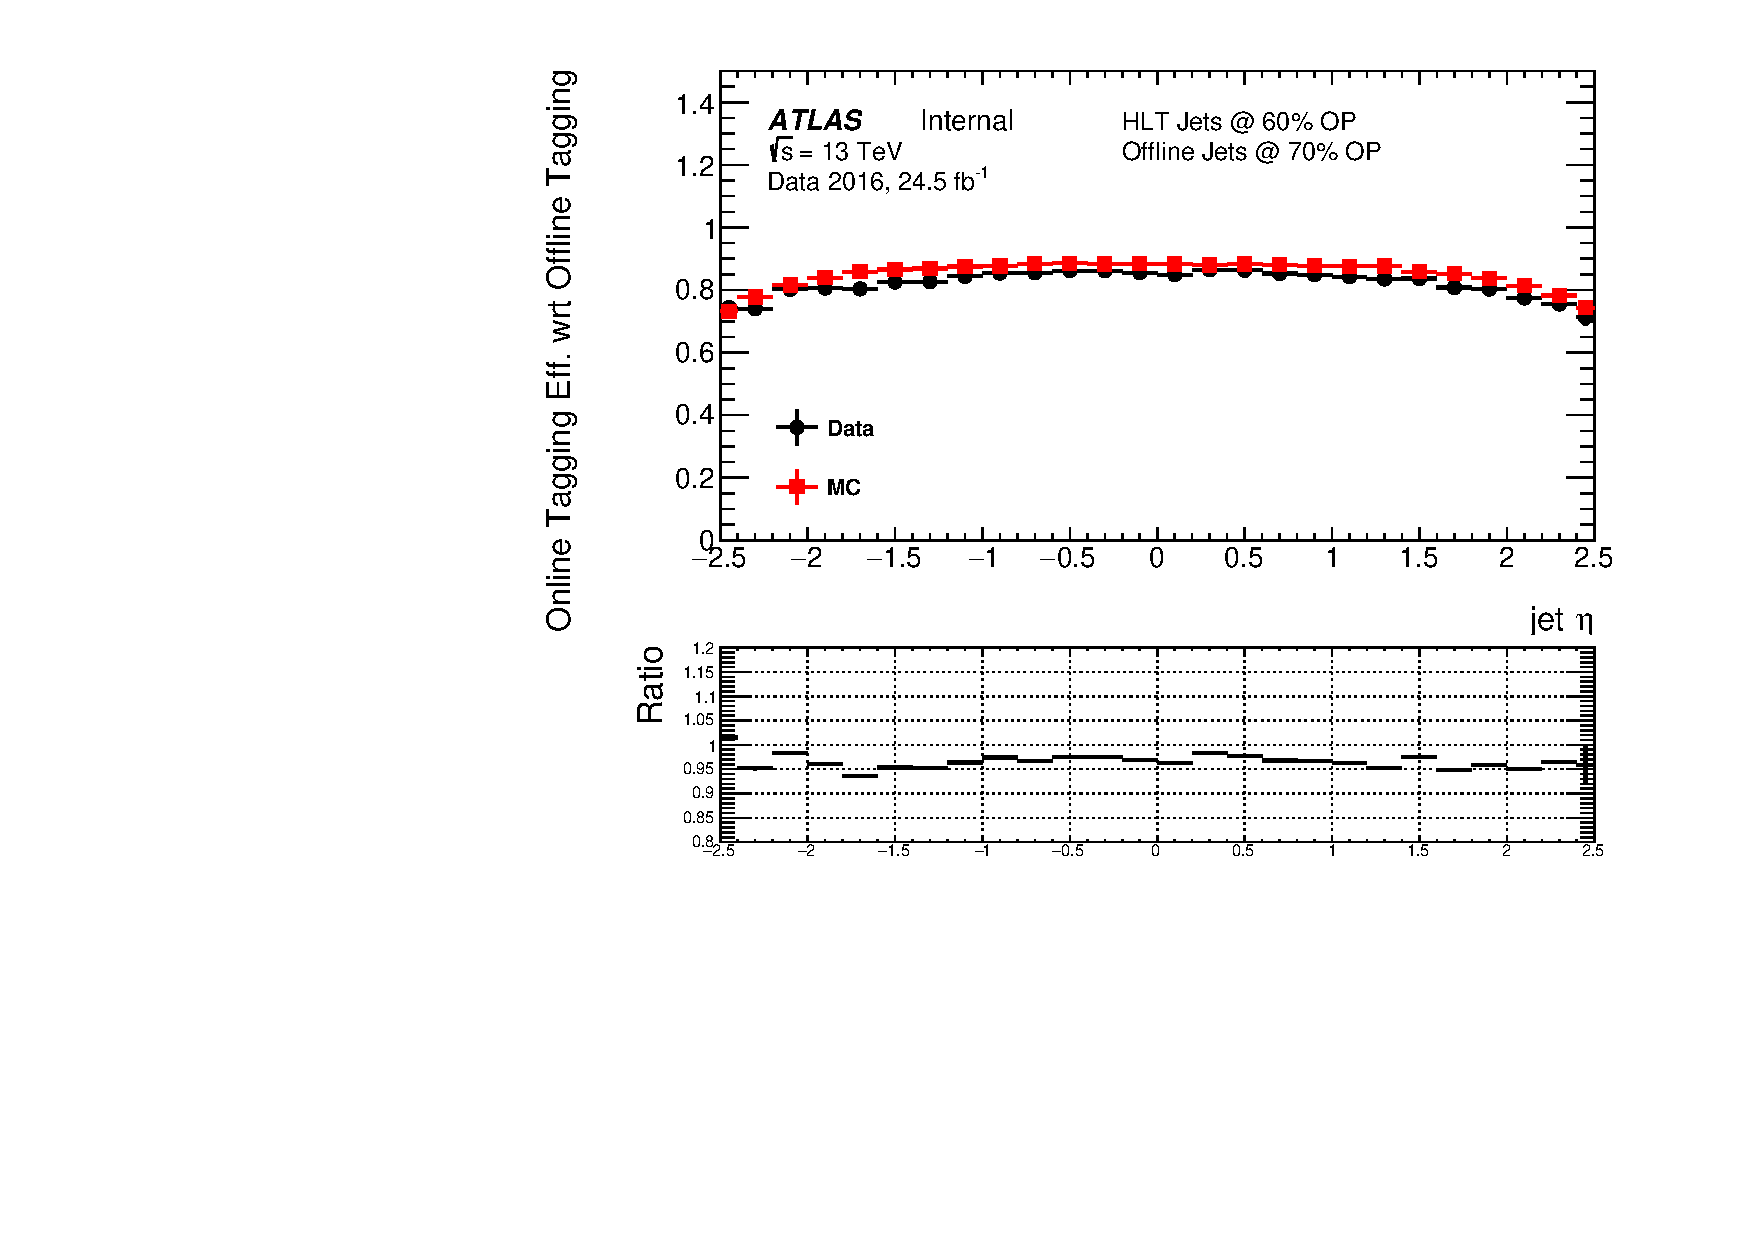
\includegraphics[width=0.47\linewidth, angle=0]{figs/Trigger/btrigger_old/Full_GRL_bslt2mm_trigReq_eff_jetEta.pdf}}\\
    \subcaptionbox{$z_{bs}^{online}$}{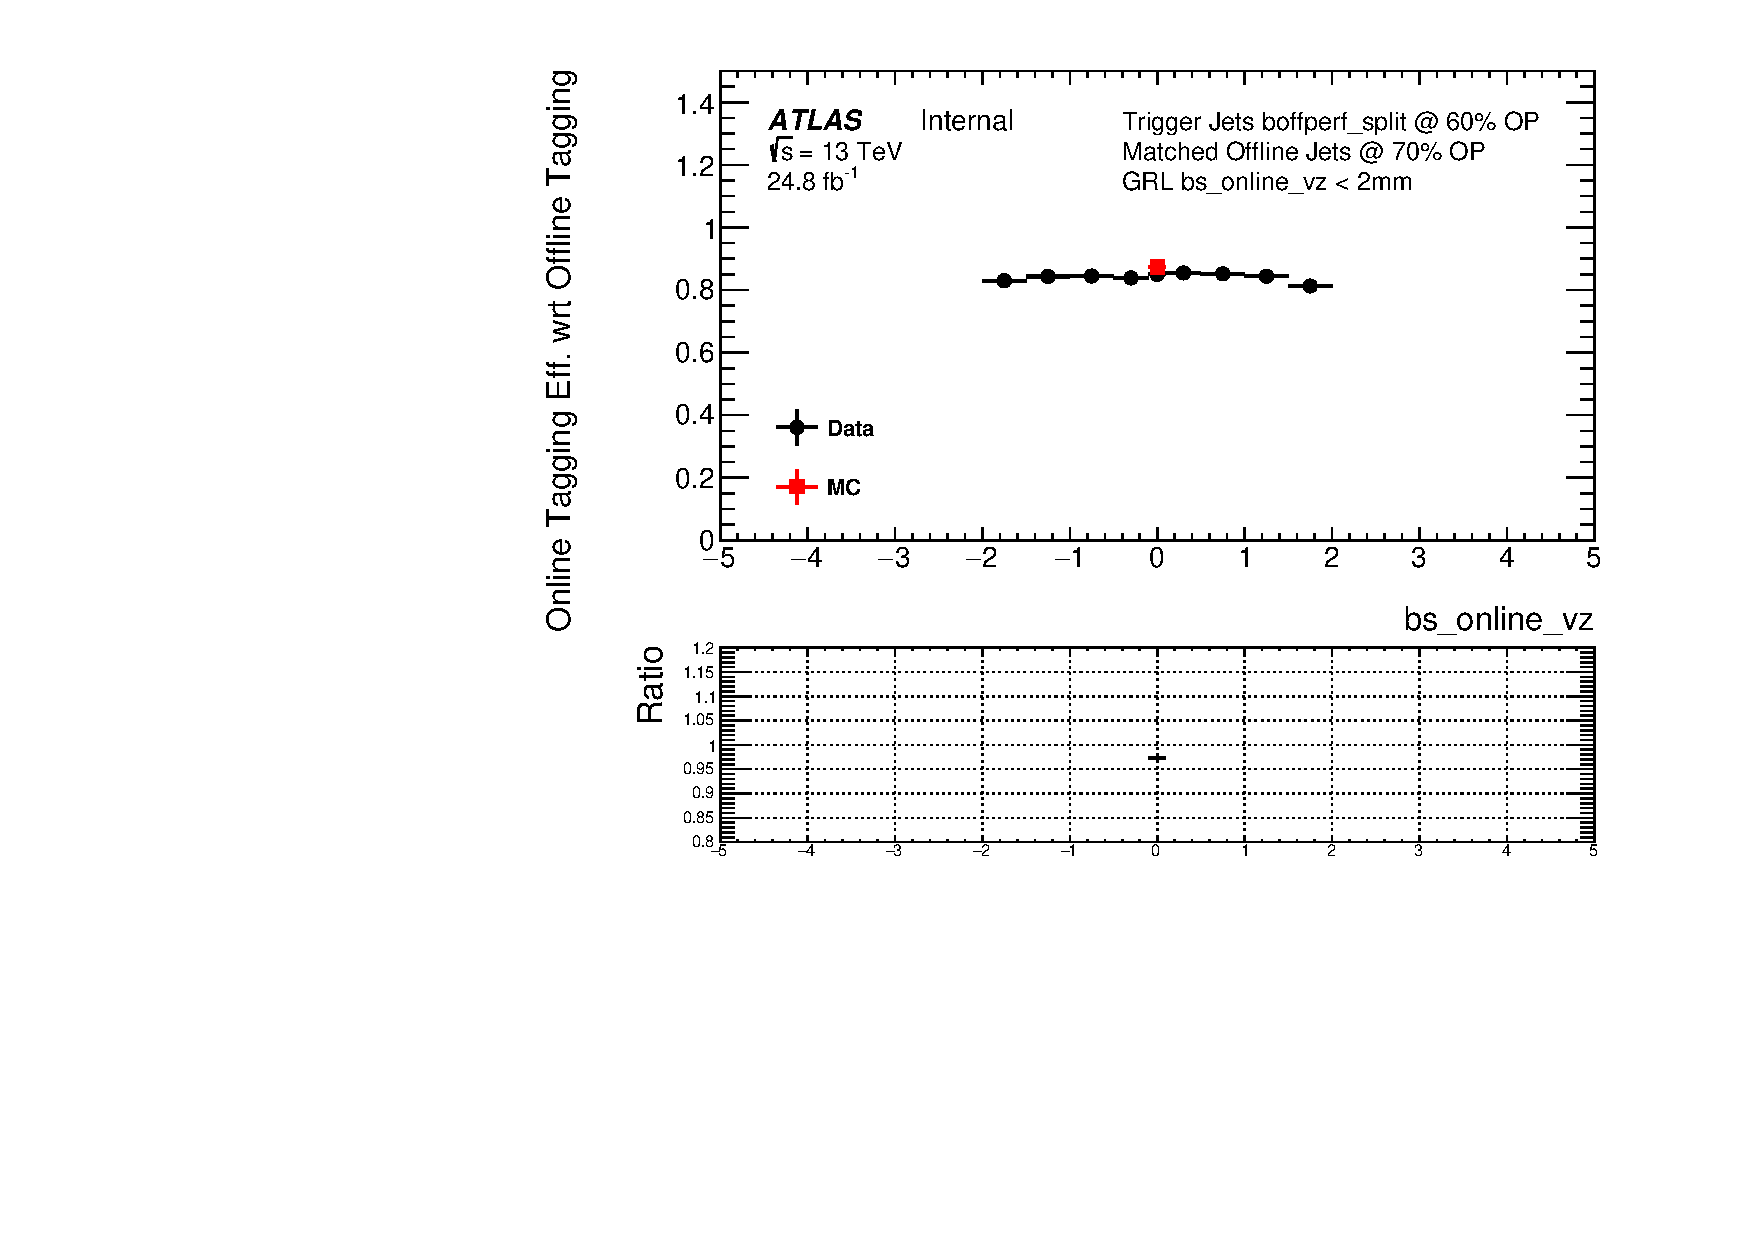
\includegraphics[width=0.47\linewidth, angle=0]{figs/Trigger/btrigger_old/Full_GRL_bslt2mm_trigReq_eff_bs_online_vz.pdf}}
    \subcaptionbox{Vertex Class}{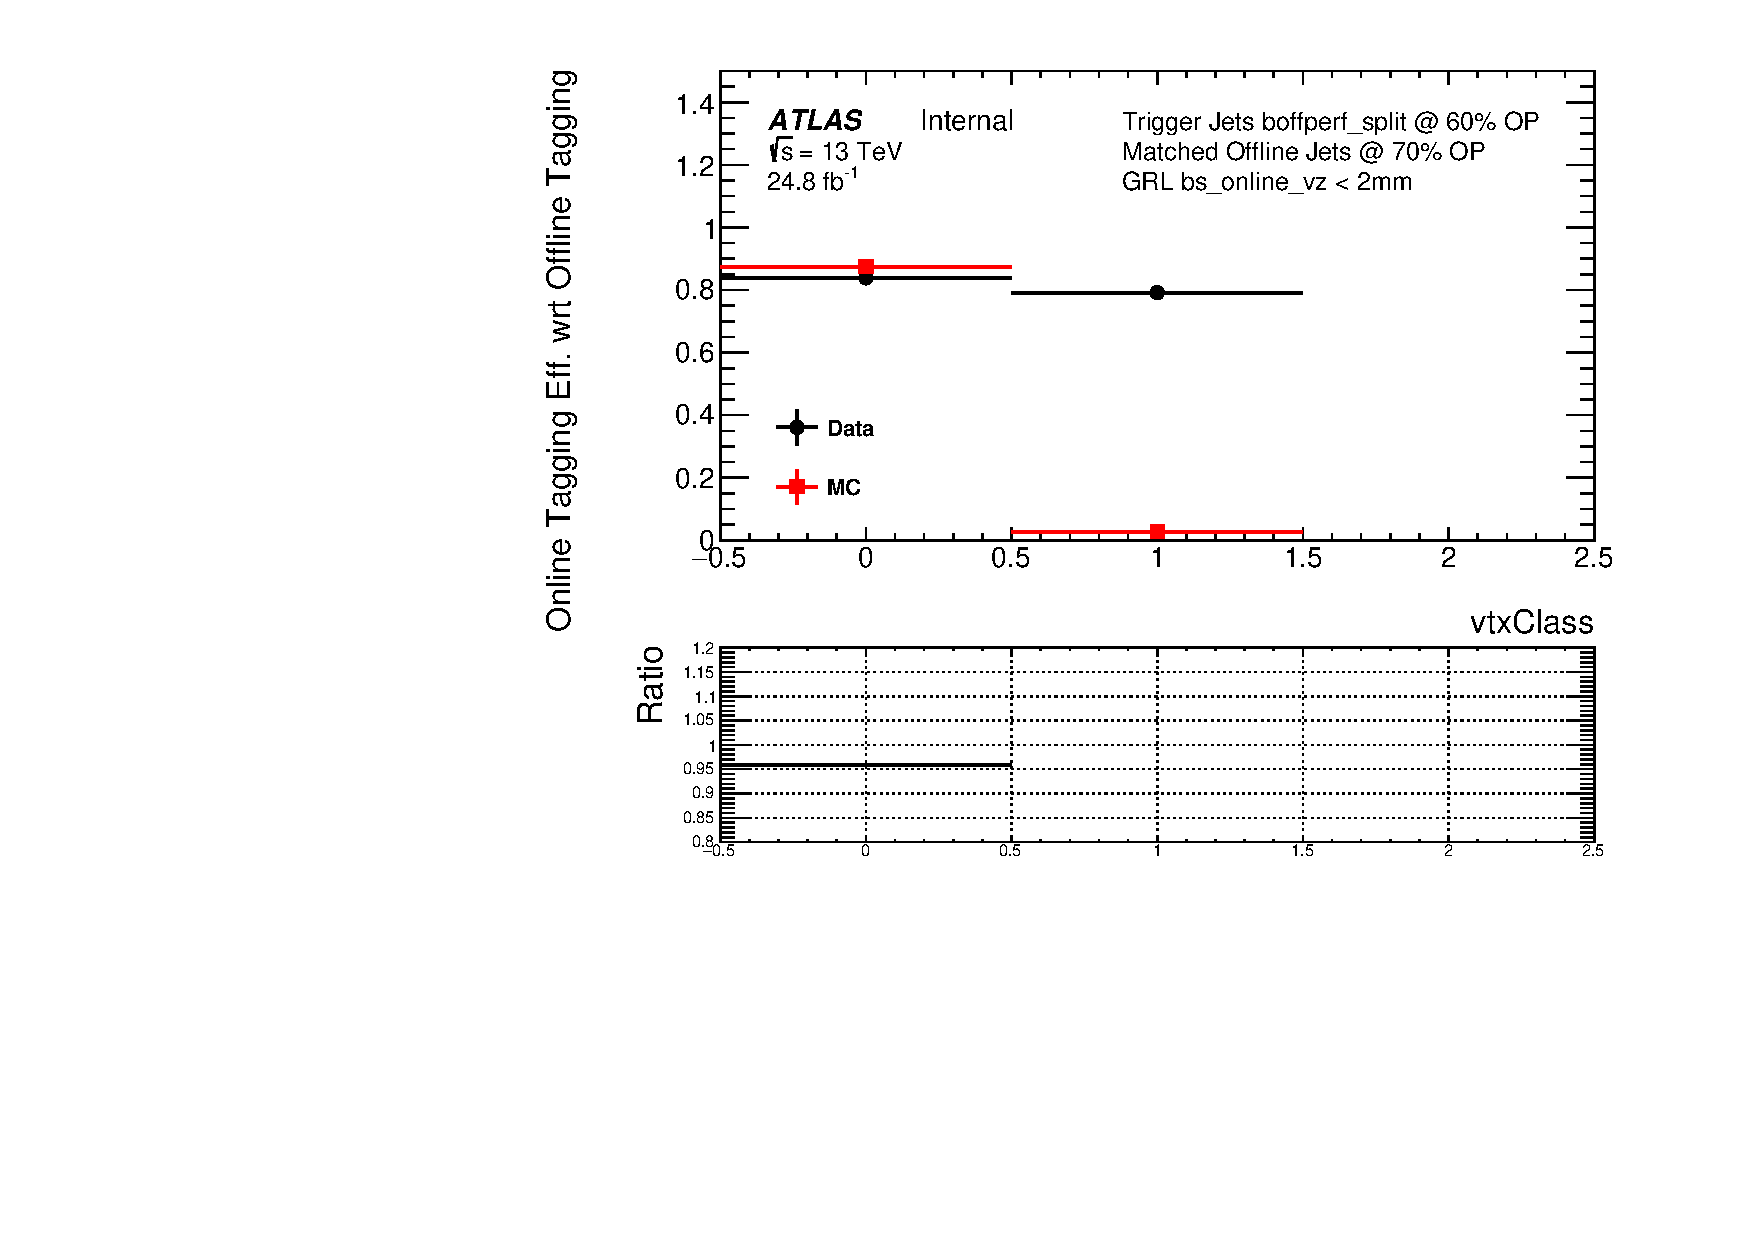
\includegraphics[width=0.47\linewidth, angle=0]{figs/Trigger/btrigger_old/Full_GRL_bslt2mm_trigReq_eff_vtxClass.pdf}}
  \end{center}
  \caption{The 60\% $b$-jet trigger efficiency with respect to an offline 70\% operating point tag
    for the full 2016 data-set (black) and simulation (red) against jet-\pT~(a), jet-$\eta$ (b), online beamspot $z$-position (c) and vertex class (d).}
  \label{fig:Full_bslt2mm_eff}
  \begin{center}
    \captionsetup[subfigure]{aboveskip=0pt,justification=centering}
    \subcaptionbox{Leading Jet-\pT}{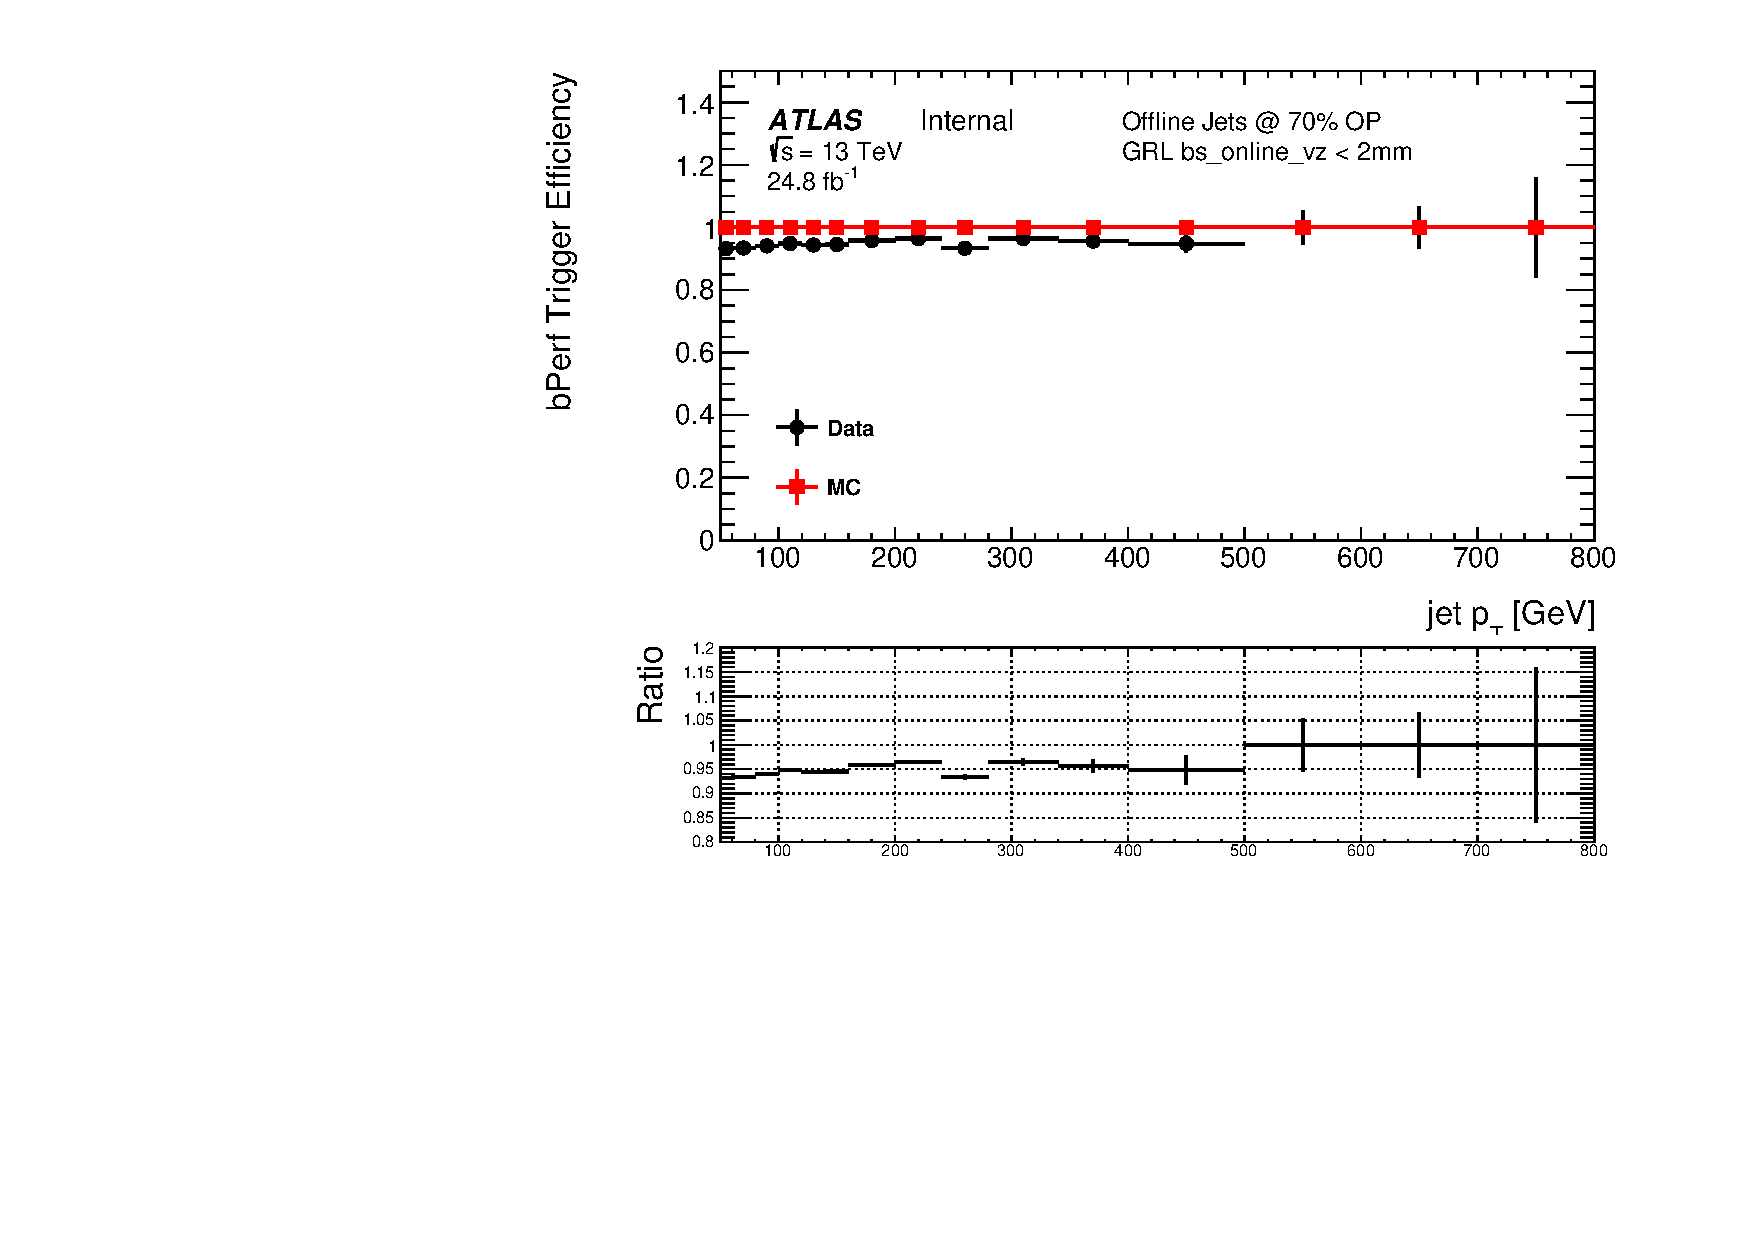
\includegraphics[width=0.47\linewidth, angle=0]{figs/Trigger/btrigger_old/Full_GRL_bslt2mm_trigReq_bPerfEff_jetPt.pdf}}
    \subcaptionbox{Leading Jet-$\eta$}{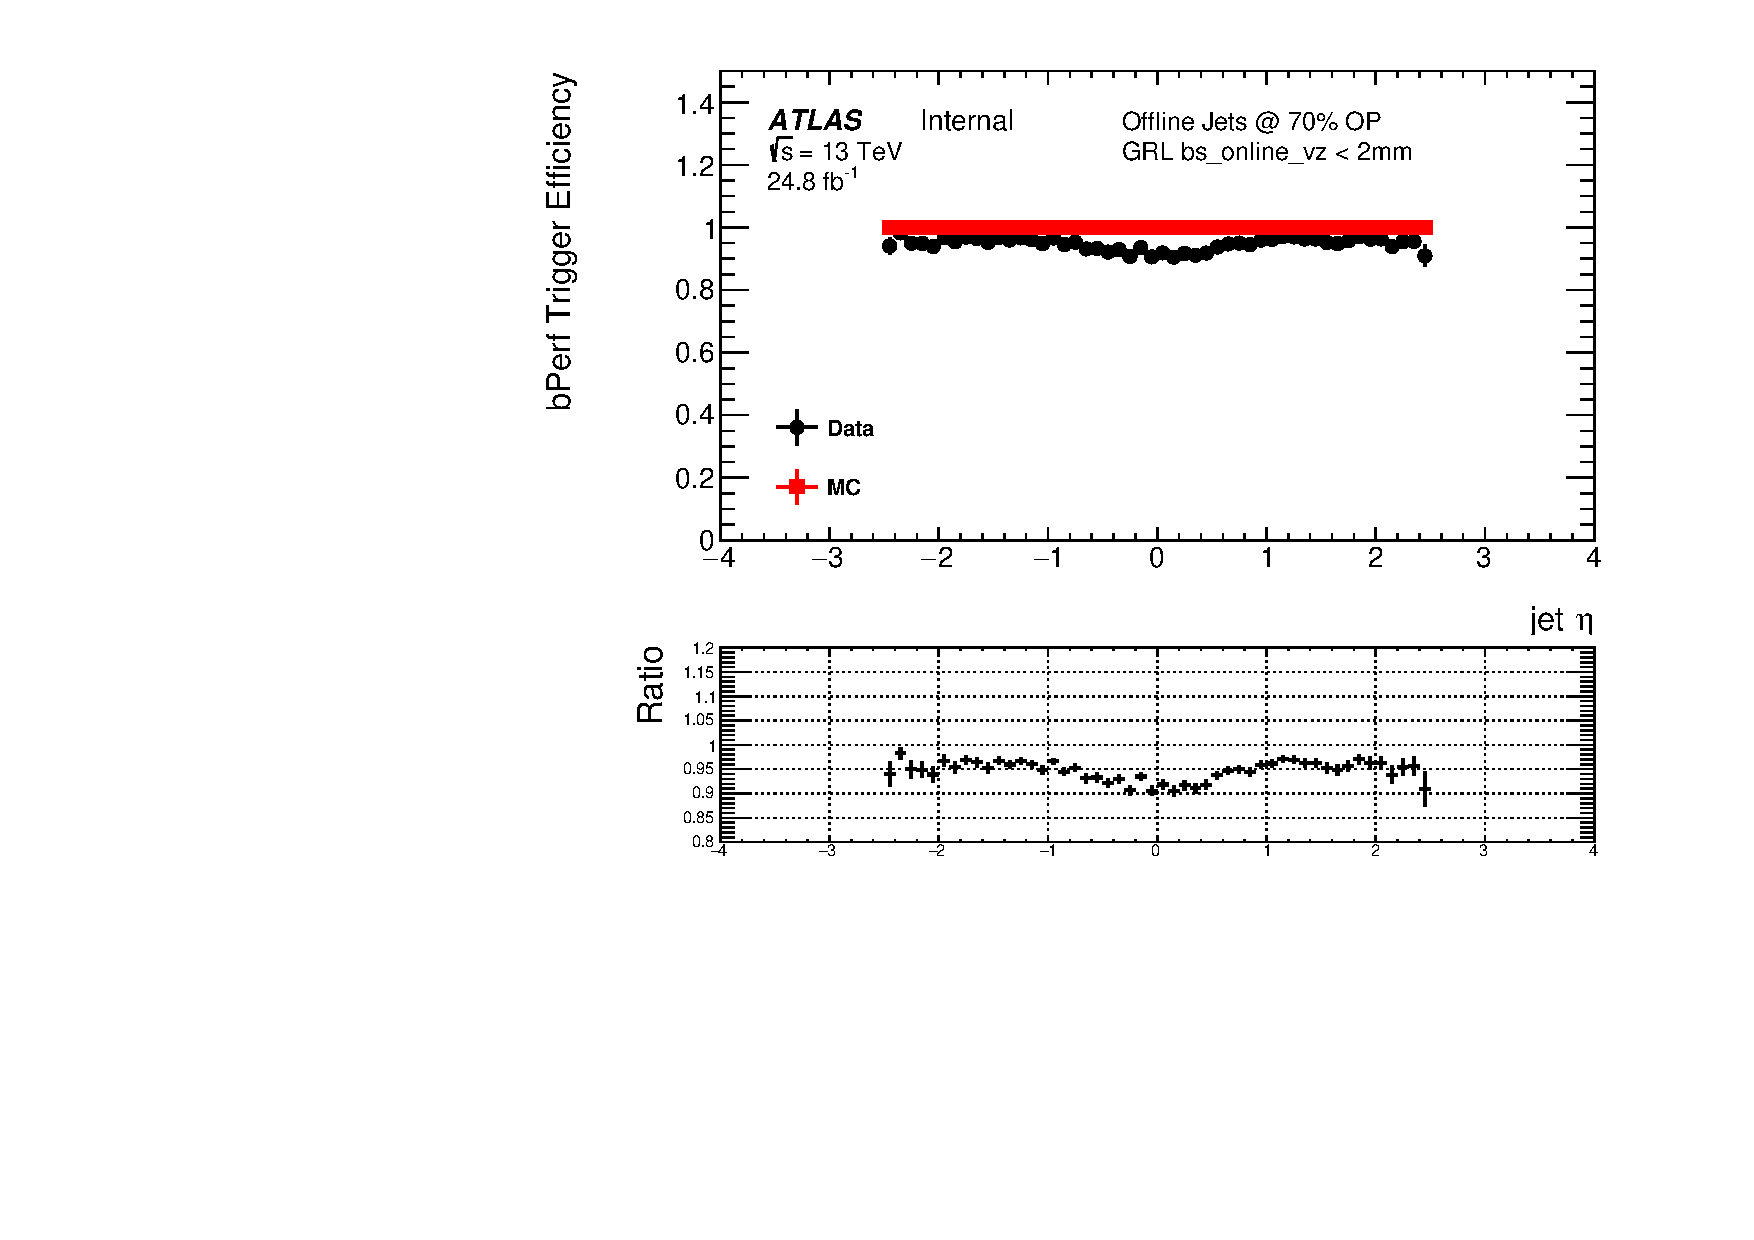
\includegraphics[width=0.47\linewidth, angle=0]{figs/Trigger/btrigger_old/Full_GRL_bslt2mm_trigReq_bPerfEff_jetEta.pdf}}
  \end{center}
  \caption{$b$-perf efficiency, $\epsilon_{bPerf}$, for the full 2016 data-set (black) and simulation (red) against (a) leading jet-\pT~and (b) jet-$\eta$.
    The $b$-jet trigger aware GRL has been applied.}
  \label{fig:Full_bslt2mm_bperf}
\end{figure}
  

\FloatBarrier
\newpage

\subsection{Efficiency Measurement and Systematic Derivation}
In the previous two sections it has been shown that when applying a $b$-jet aware GRL,
the $b$-jet trigger performance is understood and the data/simulation agreement is within 5\%.
In this section the measurement of data efficiency, data/simulation scale factors (SFs)
and associated systematics to account for the 5\% are described.

As discussed above, there are two factors considered in this section.
Firstly there is the $\epsilon_{bTrig}$ measurement
that accounts for differences in online and offline $b$-tagging given that a valid primary vertex has been found.
Sections~\ref{sec:trig-purity}~to~\ref{sec:trig-highPtExtrap} describes the derivation of a set of systematics and corrections to the raw measurement
and Section~\ref{sec:trig-jetLevelEff} presents the final measurement, which is applied as a jet-level efficiency in the final analysis.
Secondly, in Section~\ref{sec:trig-eventLevelEff}, is a description the measurement of the $\epsilon_{bPerf}$ that accounts
for the efficiency of finding a valid primary vertex and the relevant systematics, which is applied as an event level efficiency.

In this section describing the final measurement, the full 2016 data set is used,
the simulated ${t\bar{t}}$ sample includes single-top processes
and the full event selection from Section~\ref{sec:trig-evtSel} is applied.

% This section got cut and moved to jetLevelEff
%\subsubsection{$\eta$ Dependence on Efficiency}
%\label{sec:trig-etaDep}
%\begin{figure}[!ht]
%  \begin{center}
%    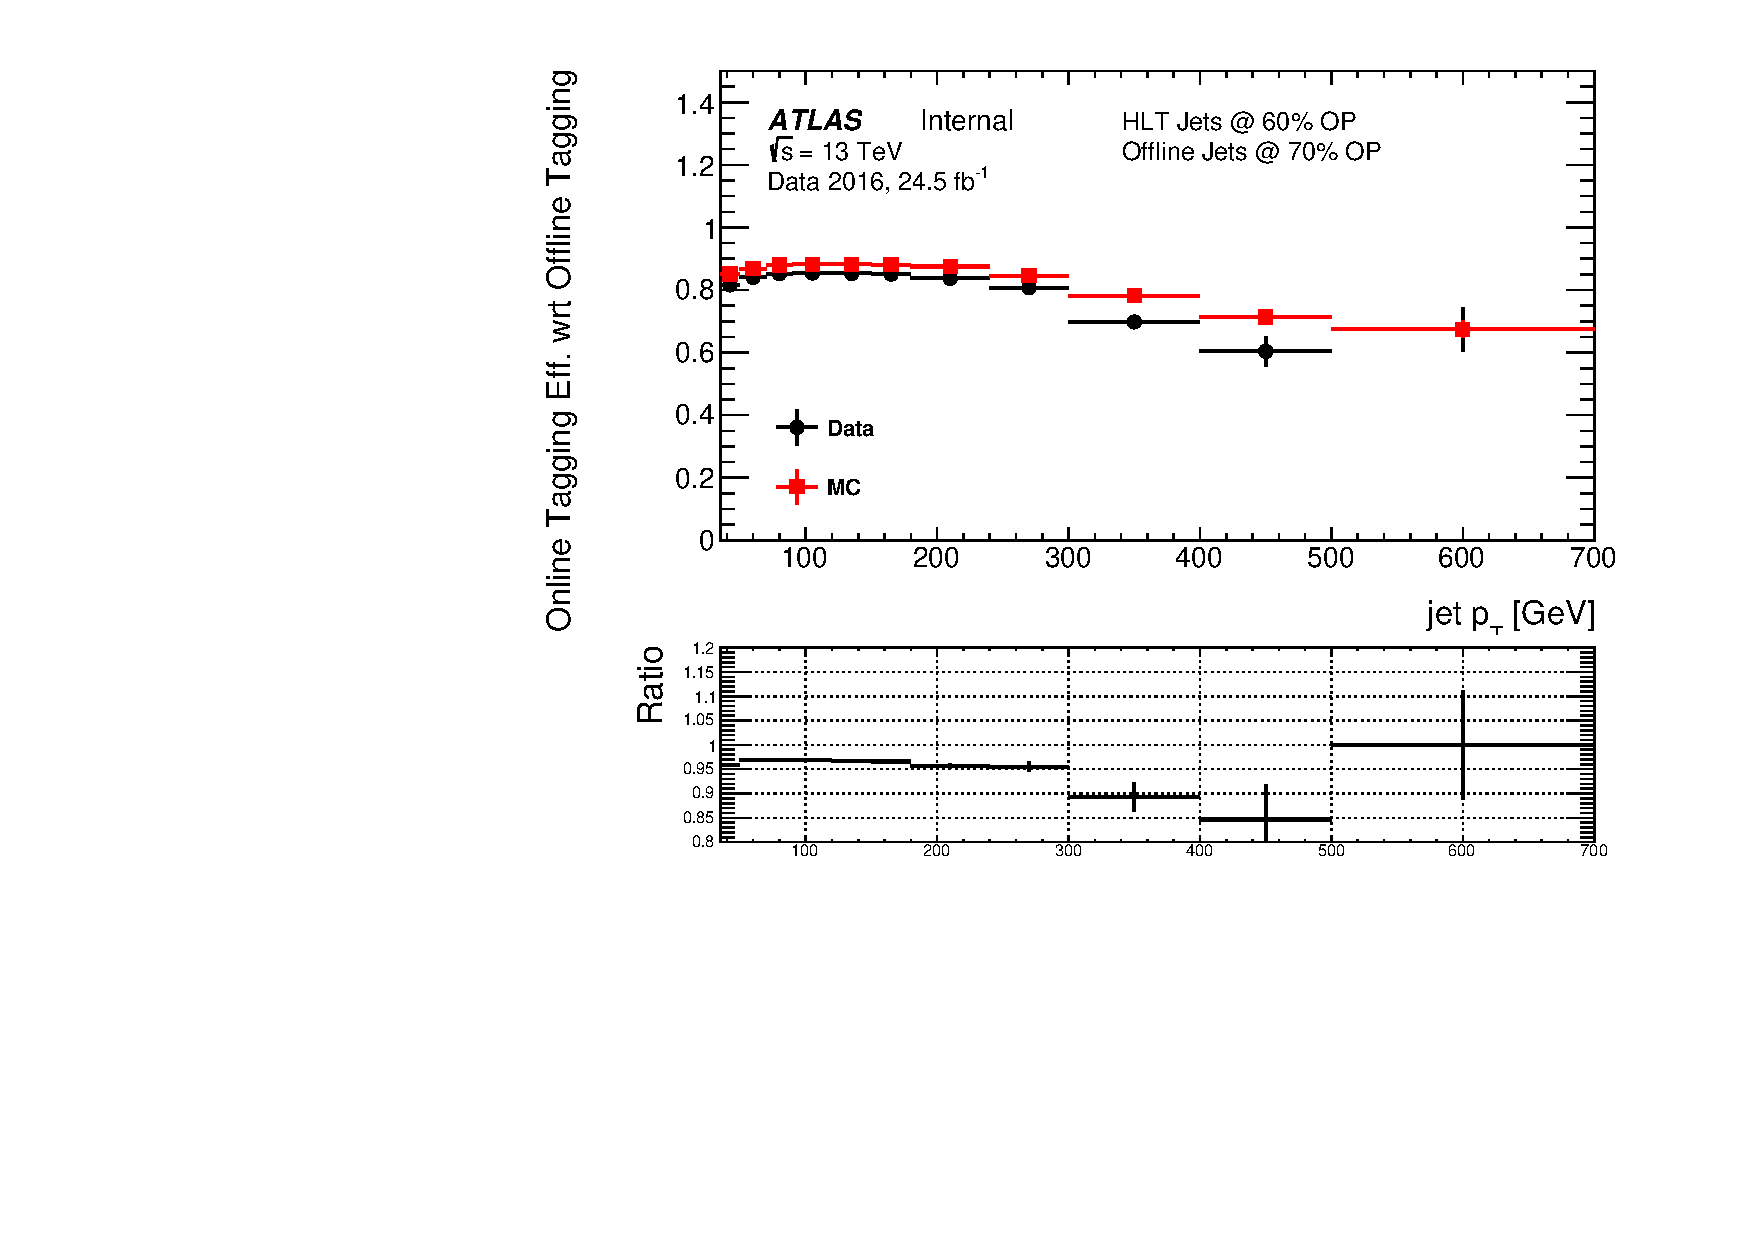
\includegraphics[width=0.47\linewidth, angle=0]{figs/Trigger/btrigger_old/Full_GRL_bslt2mm_trigReq_eff_jetPt.pdf}
%    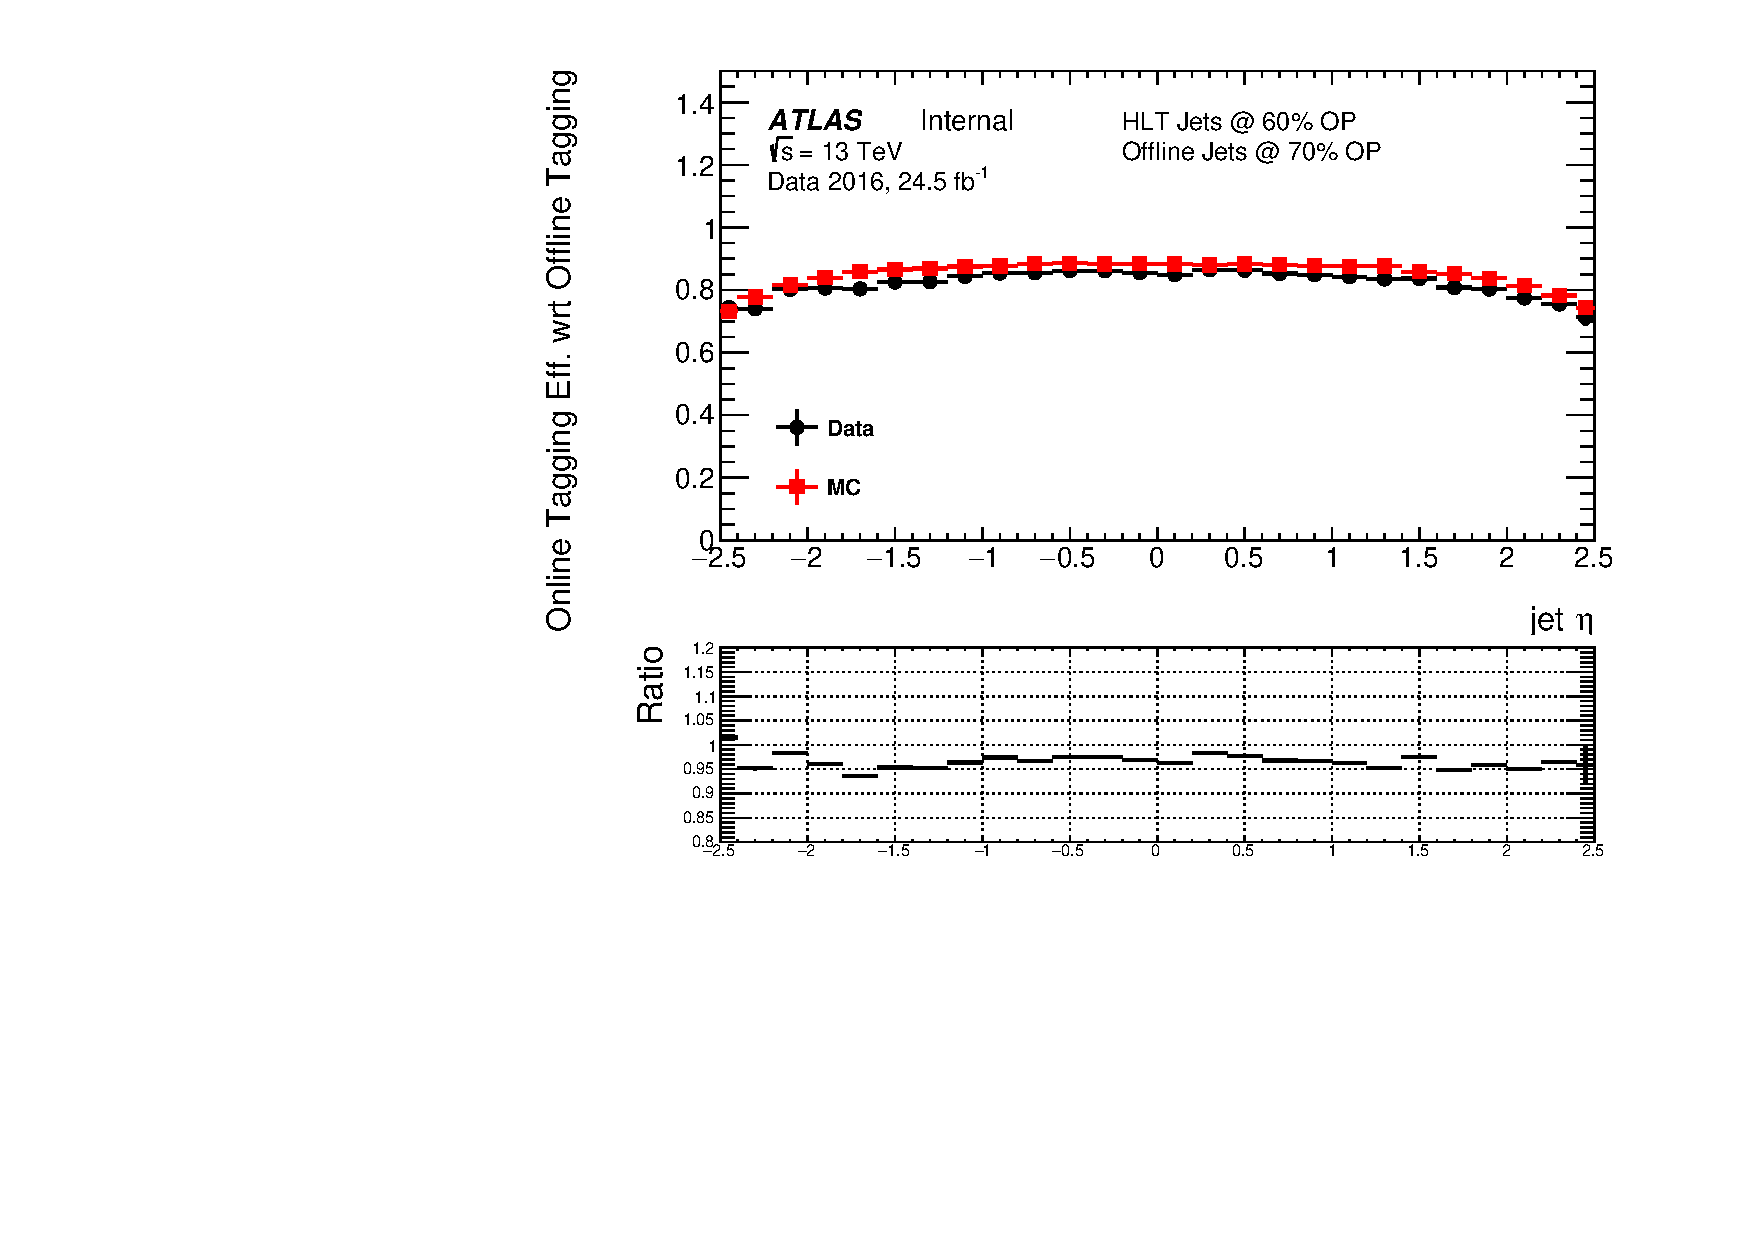
\includegraphics[width=0.47\linewidth, angle=0]{figs/Trigger/btrigger_old/Full_GRL_bslt2mm_trigReq_eff_jetEta.pdf}
%  \end{center}
%  \caption{The 60\% $b$-jet trigger efficiency with respect to an offline 70\% operating point tag
%    for data from Periods A-L (black) and simulation (red) against jet-\pT~(a), jet-$\eta$ (b).}
%  \label{fig:Full_bslt2mm_eff_eta}
%\end{figure}

\subsubsection{Purity Error}
\label{sec:trig-purity}

It is known that despite the strict event selection there will inevitably be non b-jet contamination in our sample.
To estimate the b-jet purity simulation is used, where the true flavour of the jet is available.
Jets as categorised as true $b$-jets, meaning that a $B$-hadron was found within a cone of R = 0.4, or true non-b-jets if not.
Then distributions for inclusive jets to the truth matched b-jets in the simulation sample are compared.
Figure~\ref{fig:Purity} shows the b-jet purity for jet-\pT~and jet-$\eta$;
showing that the b-jet purity is $>$ 95\% up to jet-\pT$\sim$300~\GeV~and $>$ 90\% for higher values of jet-\pT.

To estimate the effect of these impurities on the efficiency measurement simulation is again used.
Firstly, the efficiency in our nominal inclusive simulation is compared
to the efficiencies if only true-b-jets or true non-b-jets are selected,
this is shown if Figure~\ref{fig:Eff_Purity}(a).
The ratio is applied as a correction to the final efficiency measurement.
Then any mismodelling of the  $b$-jet fraction in simulation is also considered,
to account for this the efficiency for the simulated inclusive sample is compared to the efficiency when the non b-jet content has been doubled, as shown in Figure~\ref{fig:Eff_Purity}(b).
The maximum difference from the efficiency measured in the inclusive simulated sample and the cases
where there is only true b-jets and where the non b-jet content has been doubled,
shown in the two ratio plots in Figure~\ref{fig:Eff_Purity}, is taken as a symmetric systematic.

\begin{figure}[!ht]
  \begin{center}
    \captionsetup[subfigure]{aboveskip=0pt,justification=centering}
    \subcaptionbox{Jet-\pT}{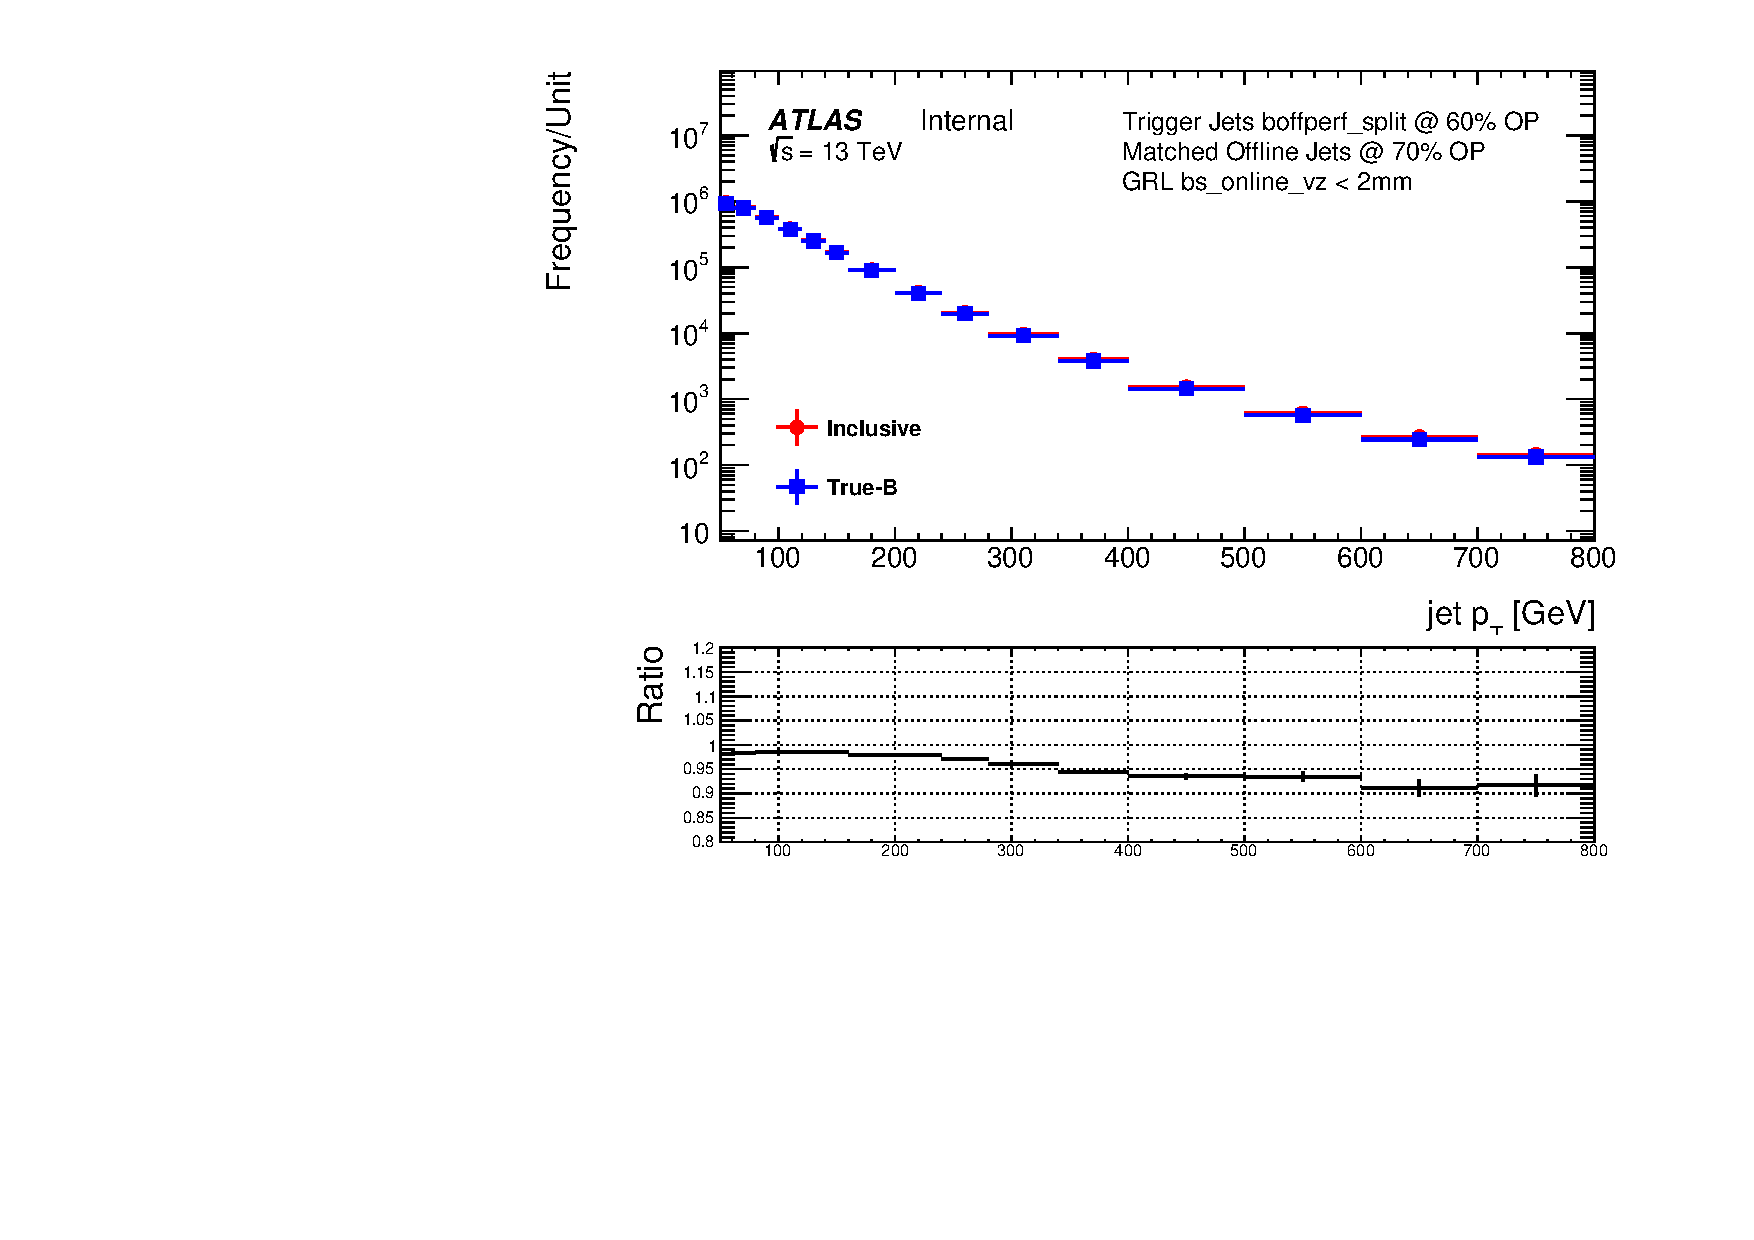
\includegraphics[width=0.47\linewidth, angle=0]{figs/Trigger/btrigger_old/PurityMC_jetPt.pdf}}
    \subcaptionbox{Jet-$\eta$}{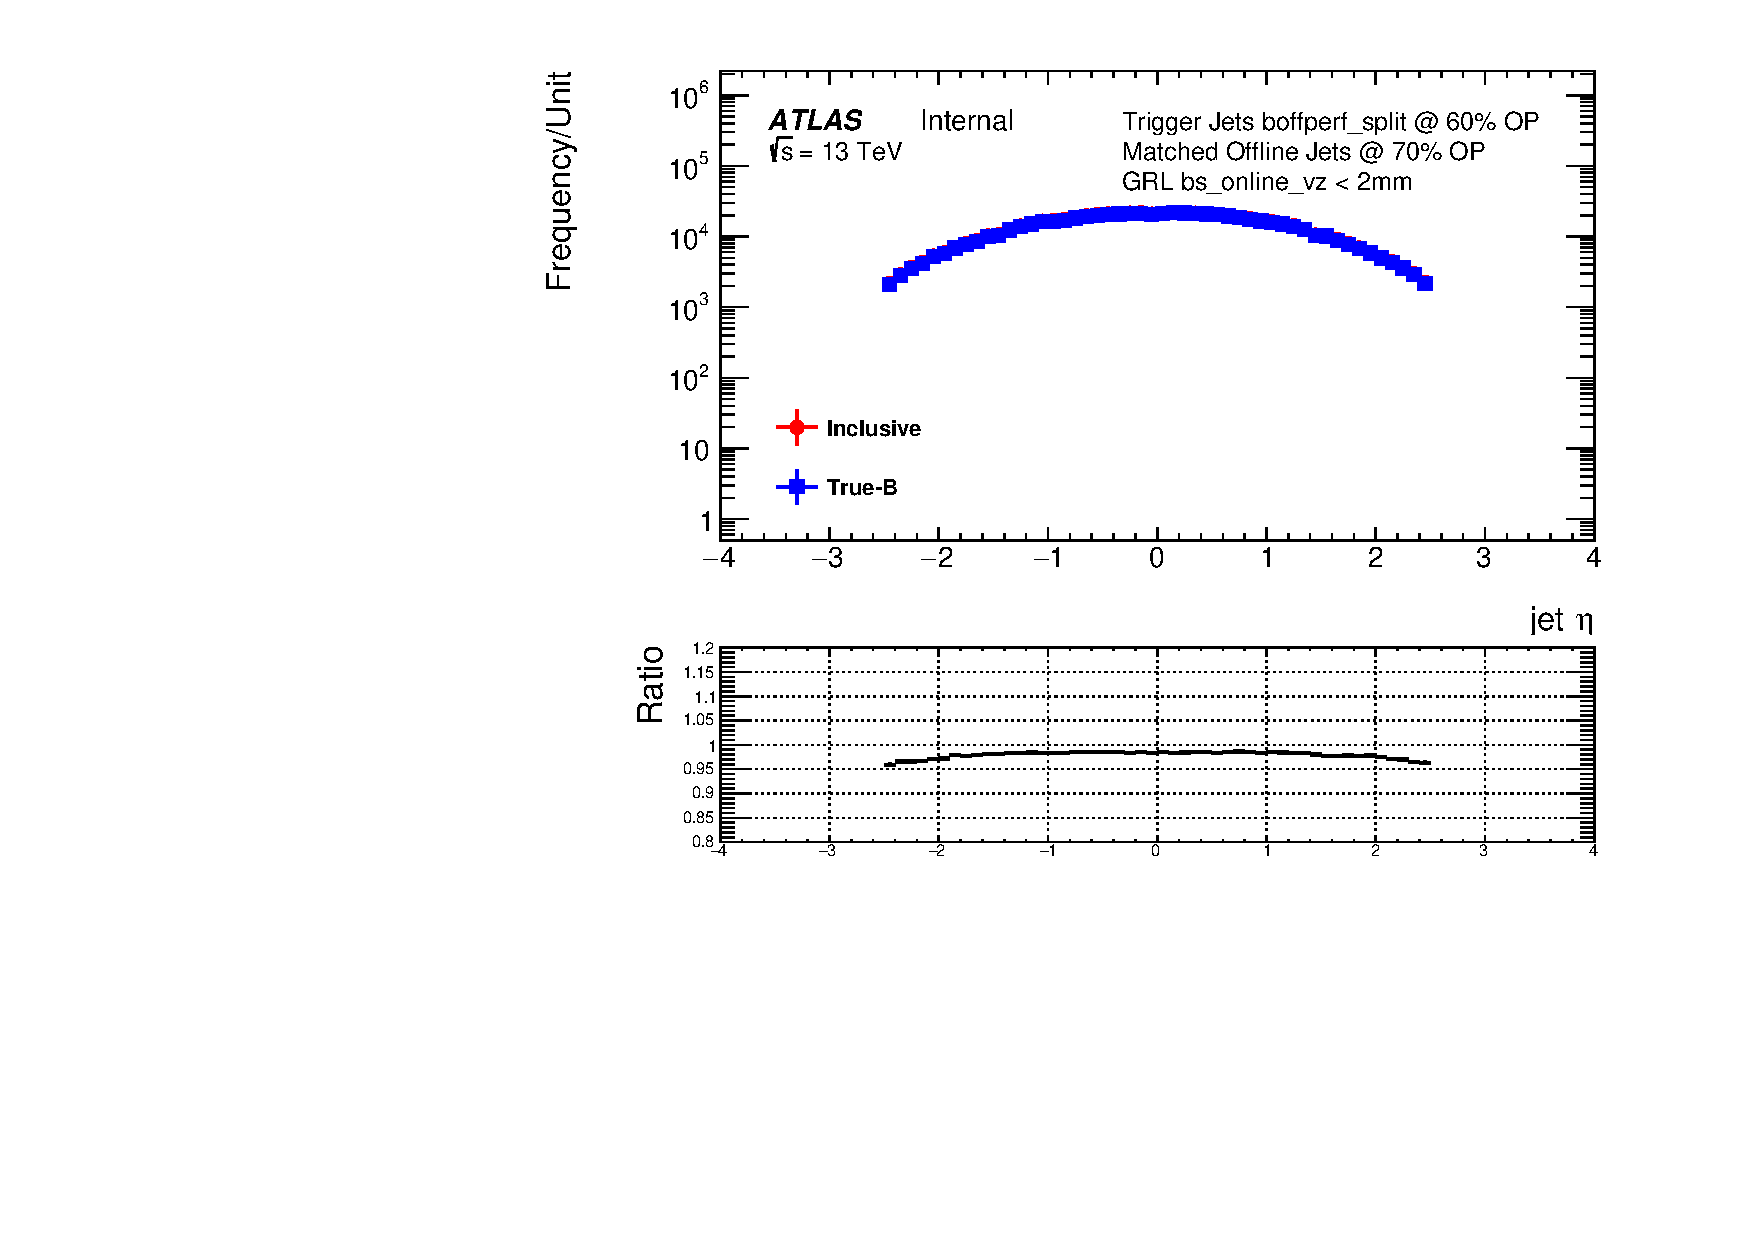
\includegraphics[width=0.47\linewidth, angle=0]{figs/Trigger/btrigger_old/PurityMC_jetEta.pdf}}
  \end{center}
  \caption{A comparison of offline jets tagged at the 70\% operating point
    for inclusive jets (red) and truth-matched b-jets (blue)
    against jet-\pT~(a) and jet-$\eta$ (b) in a simulated $t\bar{t}$ sample.}
  \label{fig:Purity}
  \begin{center}
    \captionsetup[subfigure]{aboveskip=0pt,justification=centering}
    \subcaptionbox{}{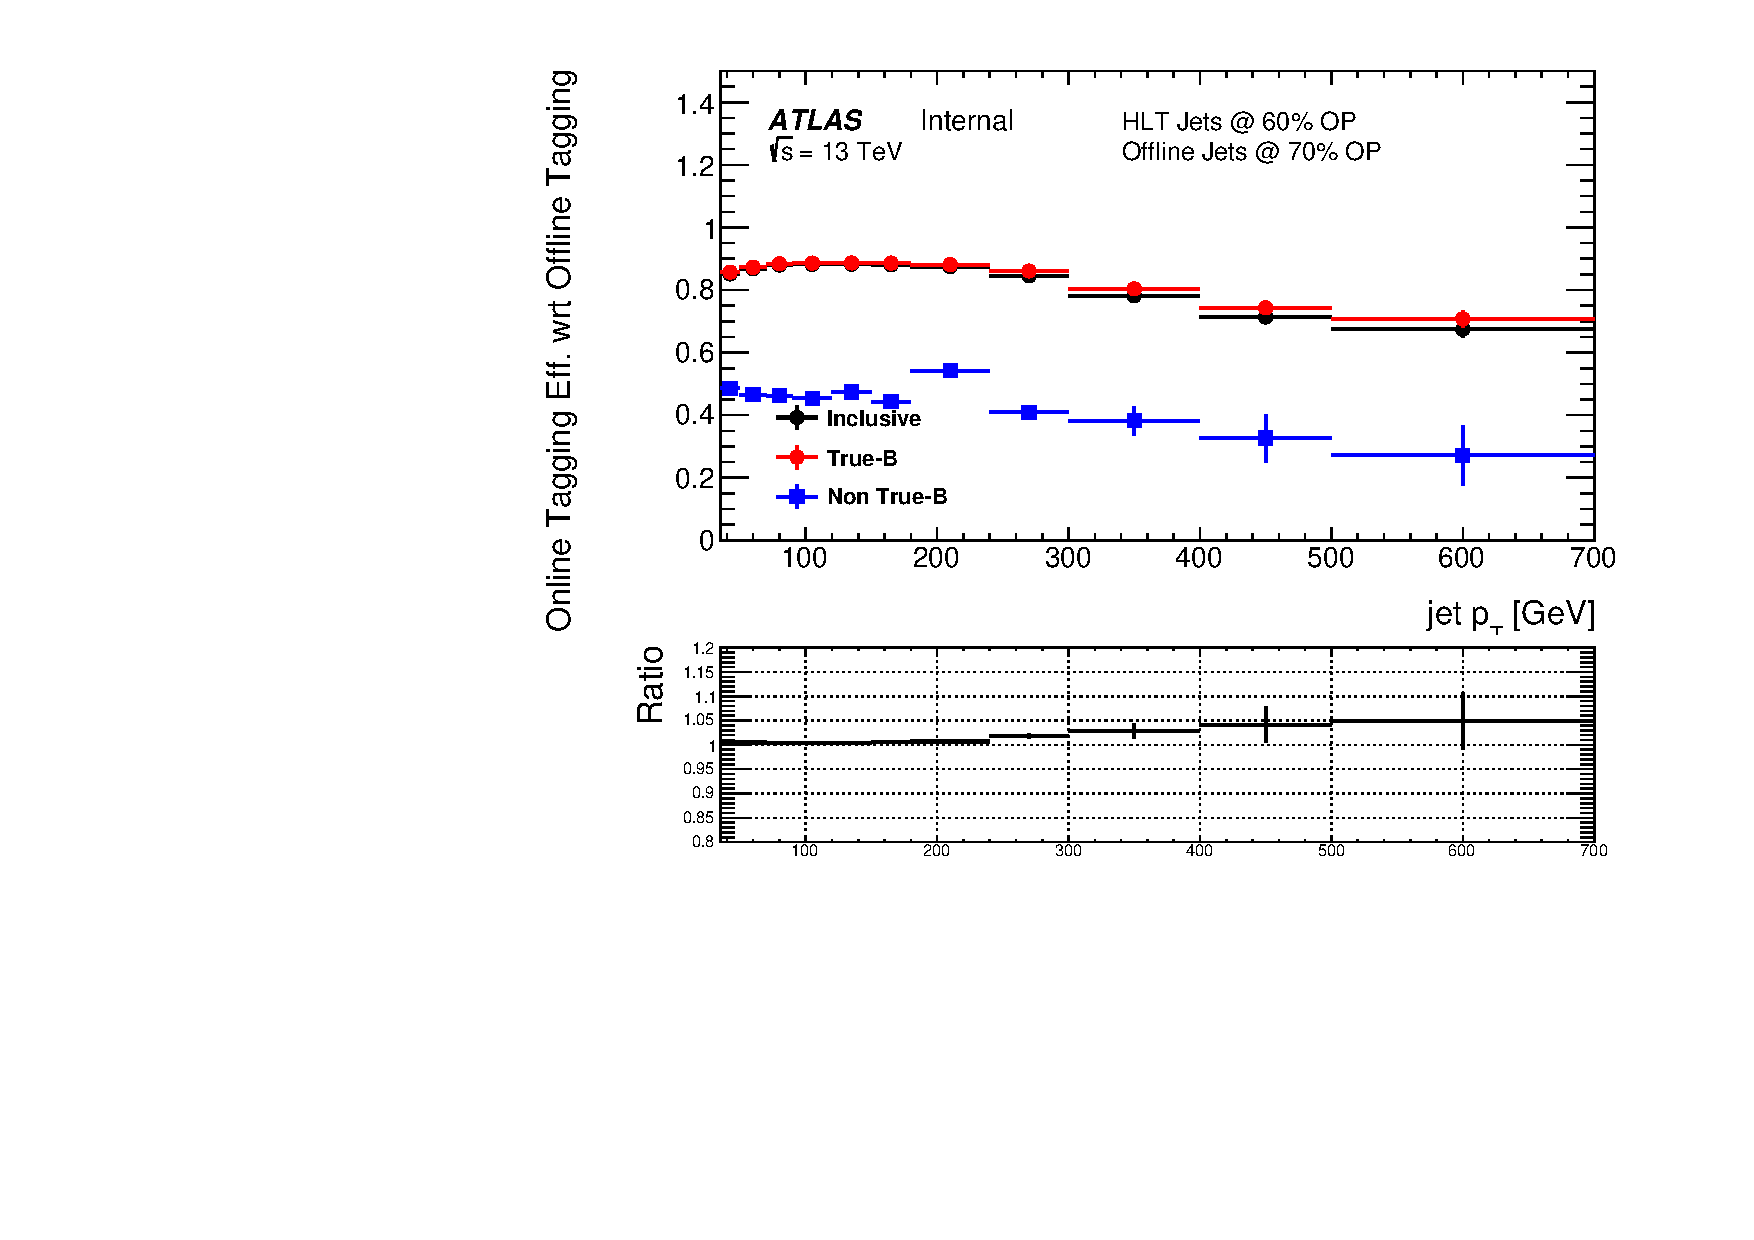
\includegraphics[width=0.47\linewidth, angle=0]{figs/Trigger/btrigger_old/EffMC_jetPt_trueB.pdf}}
    \subcaptionbox{}{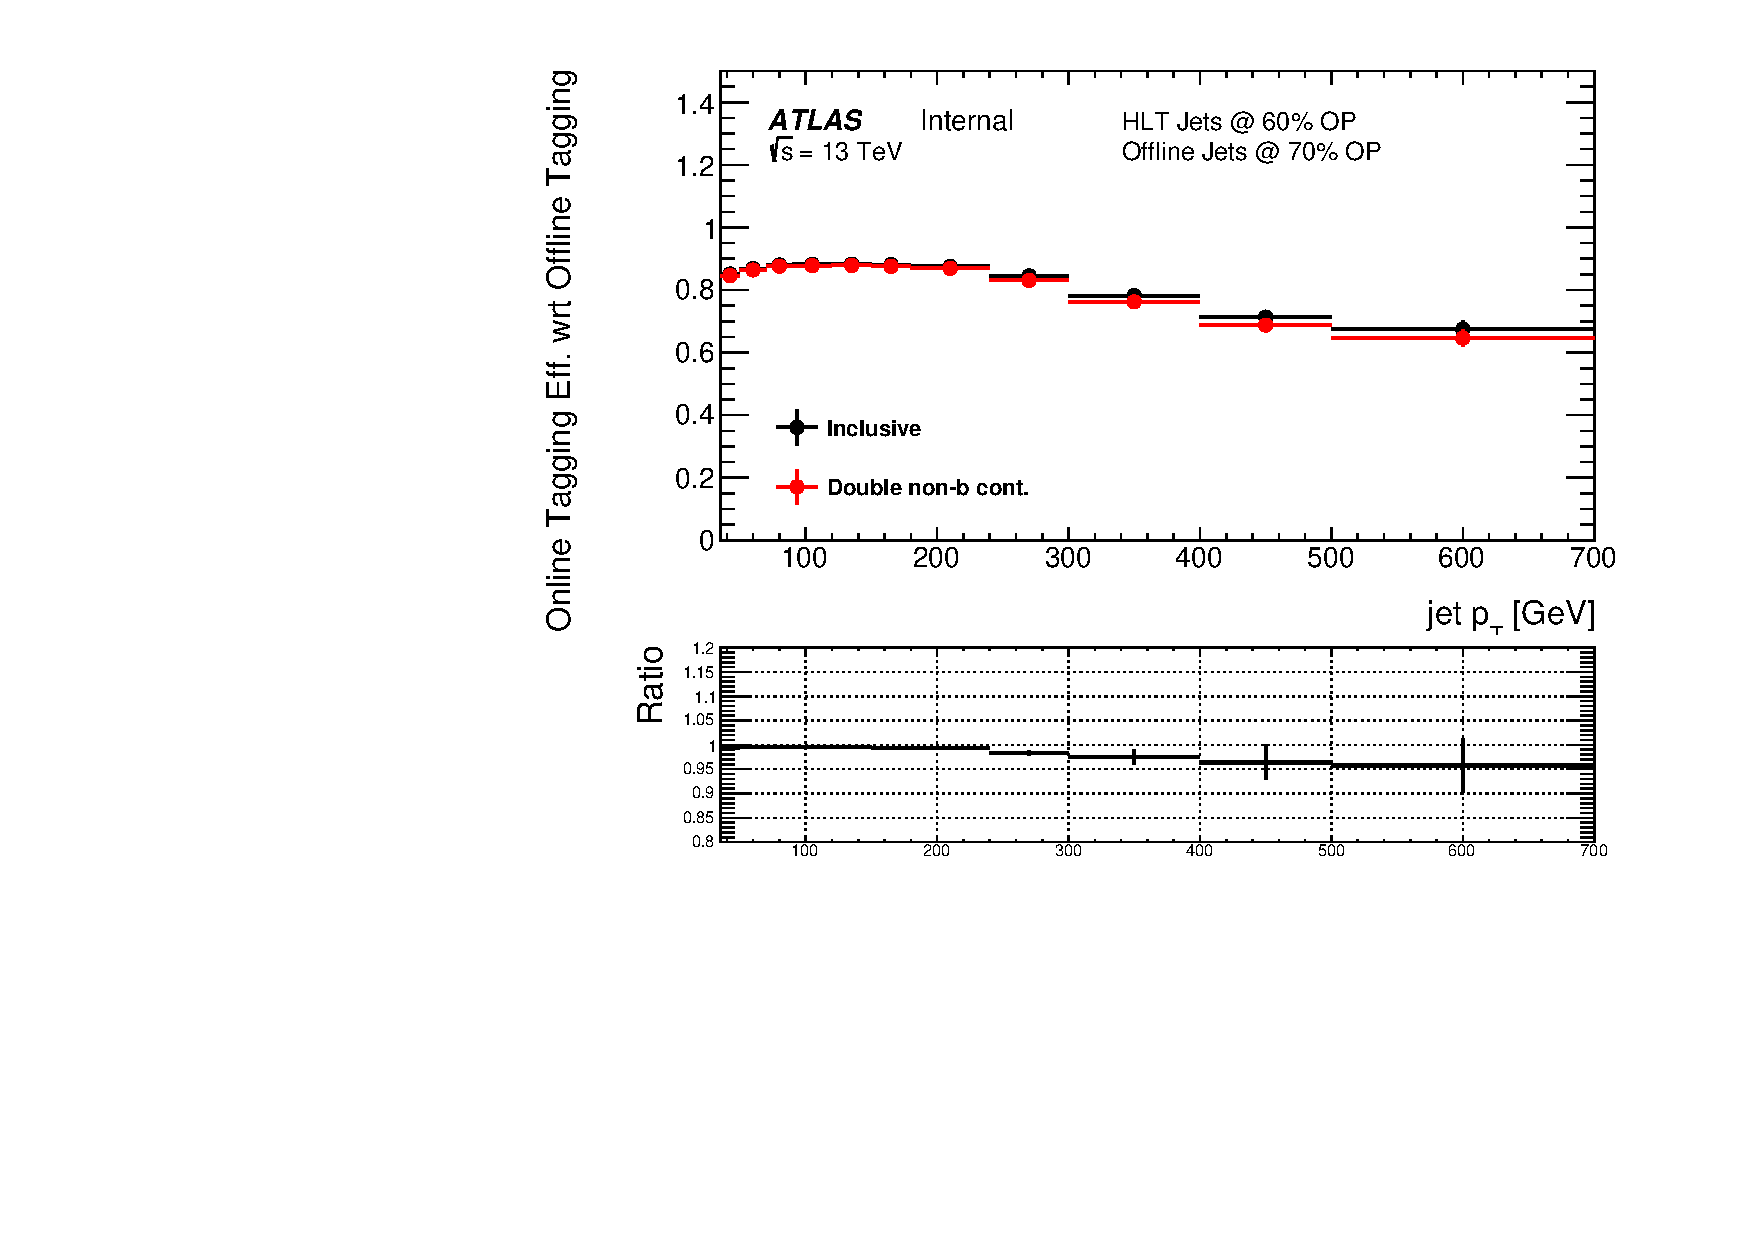
\includegraphics[width=0.47\linewidth, angle=0]{figs/Trigger/btrigger_old/EffMC_jetPt_2nonB.pdf}}
  \end{center}
  \caption{The 60\% $b$-jet trigger efficiency with respect to an offline 70\% operating point tag
    for inclusive jets (black) compared to truth matched b-jets and non b-jets (a) and the case where non b-jet content has been doubled (b) for a simulated $t\bar{t}$ sample.
    The lower panel in both plots show the ratio to the inclusive efficiency.
  }
  \label{fig:Eff_Purity}
\end{figure}

\subsubsection{Non-b-jet trigger efficiency error}
\label{sec:trig-lightTrigEff}

As one would expect and as shown in left plot of Figure~\ref{fig:Eff_Purity}, non b-jets (shown in blue) have a different b-jet trigger efficiency to that of b-jets.
However the exact efficiency is not known well and could be mismodelled in simulation.
To account for this uncertainty the nominal efficiency in simulation is compared
to the cases where the non-b-jet efficiency has been halved and doubled in simulation, as shown in Figure~\ref{fig:Eff_LTrigEff}.
When doubling the non-b-jet trigger efficiency this is limited at the upper end to being no greater than the true b-jet trigger efficiency.
The maximum bin-by-bin difference between the nominal and the two cases, as shown in the two ratio plots, is taken as a systematic.

\begin{figure}[!ht]
  \begin{center}
    \captionsetup[subfigure]{aboveskip=0pt,justification=centering}
    \subcaptionbox{}{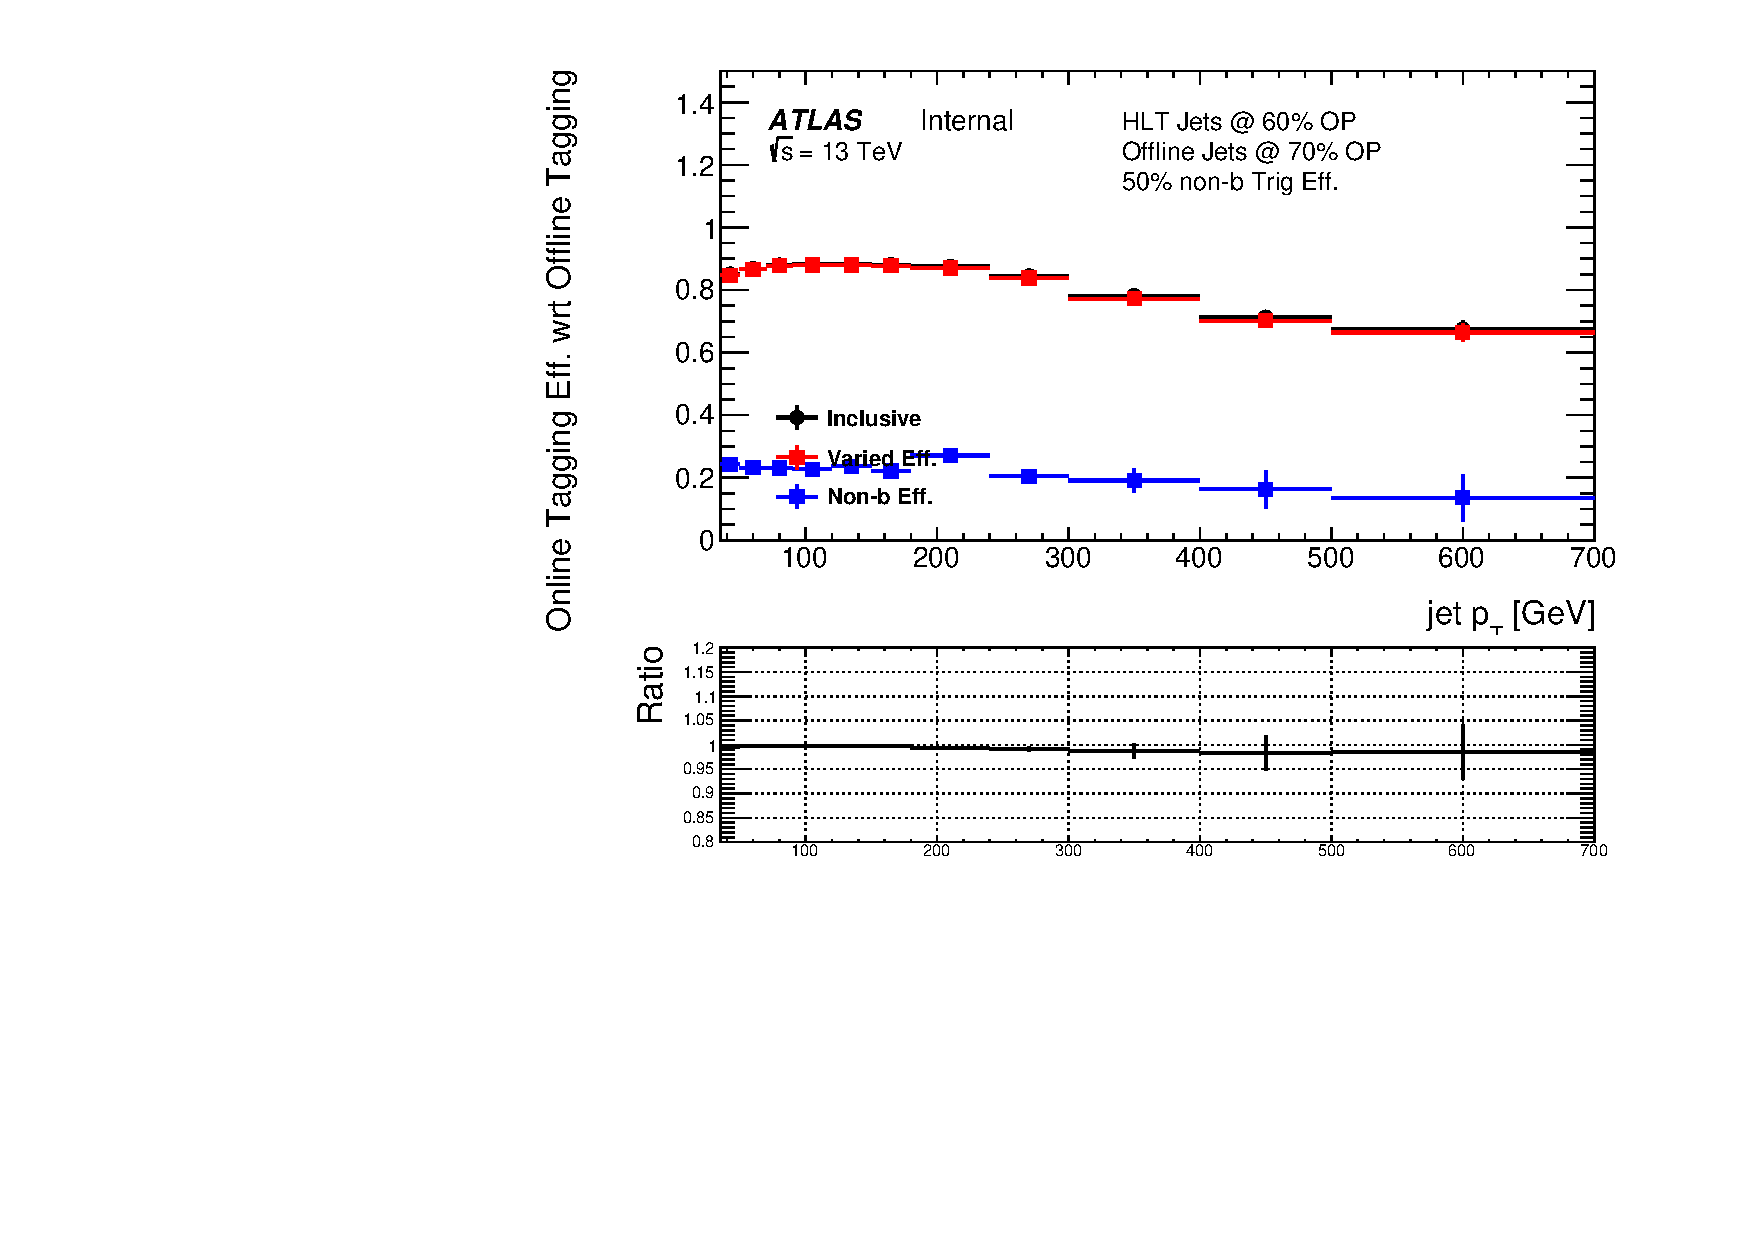
\includegraphics[width=0.47\linewidth, angle=0]{figs/Trigger/btrigger_old/effMC_jetPt_lowLTrigEff.pdf}}
    \subcaptionbox{}{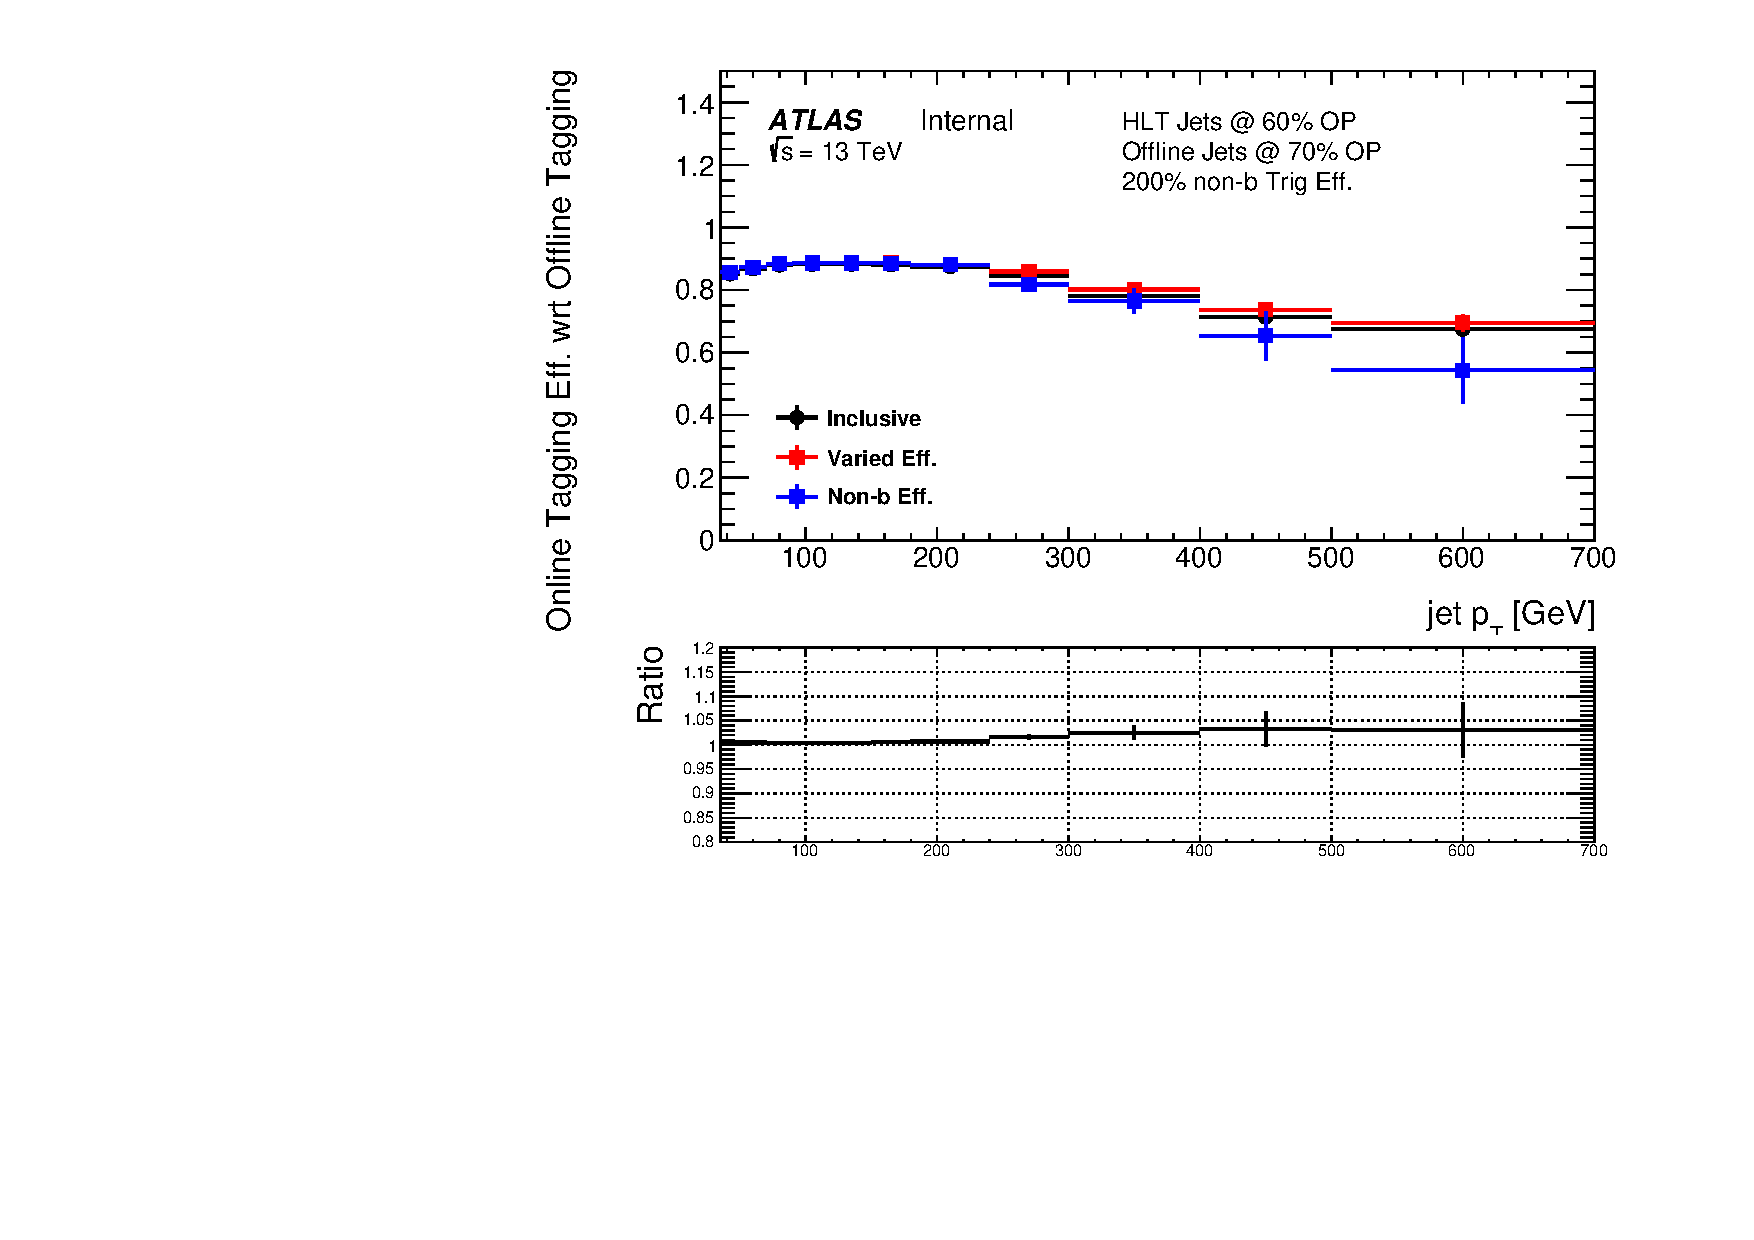
\includegraphics[width=0.47\linewidth, angle=0]{figs/Trigger/btrigger_old/effMC_jetPt_upLTrigEff.pdf}}
  \end{center}
  \caption{The 60\% $b$-jet trigger efficiency with respect to an offline 70\% operating point tag
    for nominal inclusive case (black) compared to varied inclusive case (red) and just non b-jets (blue)
    in the case where non b-jet efficiency has been halved (a) and doubled (b) for a simulated $t\bar{t}$ sample.
    The lower panel in both plots show the ratio of the varied inclusive efficiency to the nominal inclusive efficiency.
  }
  \label{fig:Eff_LTrigEff}
\end{figure}

\FloatBarrier

\subsubsection{High-\pT~extrapolation}
\label{sec:trig-highPtExtrap}

Measuring $b$-jet trigger efficiency for high-\pT~jets is limited by the statistics in the simulated $t\bar{t}$ sample,
so the shape from simulation will be used to extrapolate the efficiency for jet-\pT $>$ 240 GeV.
The point from which to extrapolate from was chosen as this is when data statistic error starts to become large. 

The procedure is made of two sequential fits (normalisation and correction) to the data/simulation ratio,
which are used to create a ``corrected simulation'' $\epsilon_{bTrig}$ distribution.
For jet-$pT$ $>$ 240 GeV, the corrected $\epsilon_{bTrig}$ is used in place of data when measuring the data $\epsilon_{bTrig}$ efficiency
and when calculating data/MC scale factors.
A final quadratic fit is used to assign a systematic. 

\noindent
In more detail:
\begin{itemize}
  \setlength\itemsep{1em}
\item \textbf{Flat Normalisation Fit}: \\
  The measured $\epsilon_{bTrig}$, in both data and simulation are compared,
  and a horizontal fit is performed to the ratio of the two.
  The fit range is set at $\pT > 50\GeV$ to discount the first bin, which has a larger purity uncertainty.
  This is then used to normalise the simulated efficiency distribution to match data.
  This fit is shown in the lower plot  of panel (a) in Figure~\ref{fig:bTrig_mcExtrap}.
  The error on the one parameter of this fit is taken as a systematic error.
  
\item \textbf{Linear Correction Fit}:  \\
  The measured $\epsilon_{bTrig}$, in both data and the normalised simulation are compared,
  and a linear fit is performed to the ratio of the two from jet-\pT $>$ 240 GeV.
  This is then used to correct the simulated efficiency distribution to match data.
  This fit is shown in the lower plot of panel (b) in Figure~\ref{fig:bTrig_mcExtrap}.
  The simulated $\epsilon_{bTrig}$, after both the normalisation and linear correction is referred to as the corrected simulation.
  To assign a systematic on the fit parameters, the slope of this fit is varied up and down within errors,
  whilst the point at which the fit crosses 1 is kept constant.
  The maximum difference between the nominal fit and the varied fits is taken as the error on the linear correction fit.
  Panel (c) of Figure~\ref{fig:bTrig_mcExtrap} shows the data compared to the corrected simulation.
  The lower panel shows the ratio of the two, and the blue lines represent the errors on the linear correction fit.
  
\item \textbf{Quadratic Systematic Fit}: \\
  Finally to assess an error on the choice of a linear fit as the functional form above,
  a fit is performed to the data and corrected simulation ratio using a quadratic function.
  This ratio and the fit is shown in panel (d) of Figure~\ref{fig:bTrig_mcExtrap}.
  The difference of the fit from 1 is considered as the functional form error when assigning as systematic.
  
\end{itemize}

The systematic error on the extrapolation is defined as the error from normalisation fit
added to the bin-by-bin maximum of the error from the linear correction fit and the error from the quadratic systematic fit.
The errors on the high-\pT~extrapolation procedure are summarised in Table~\ref{tab:bTrig_extrapSyst}
  
\begin{figure}[!ht]
\begin{center}
\captionsetup[subfigure]{aboveskip=0pt,justification=centering}
  \subcaptionbox{Data/MC with normalisation fit} {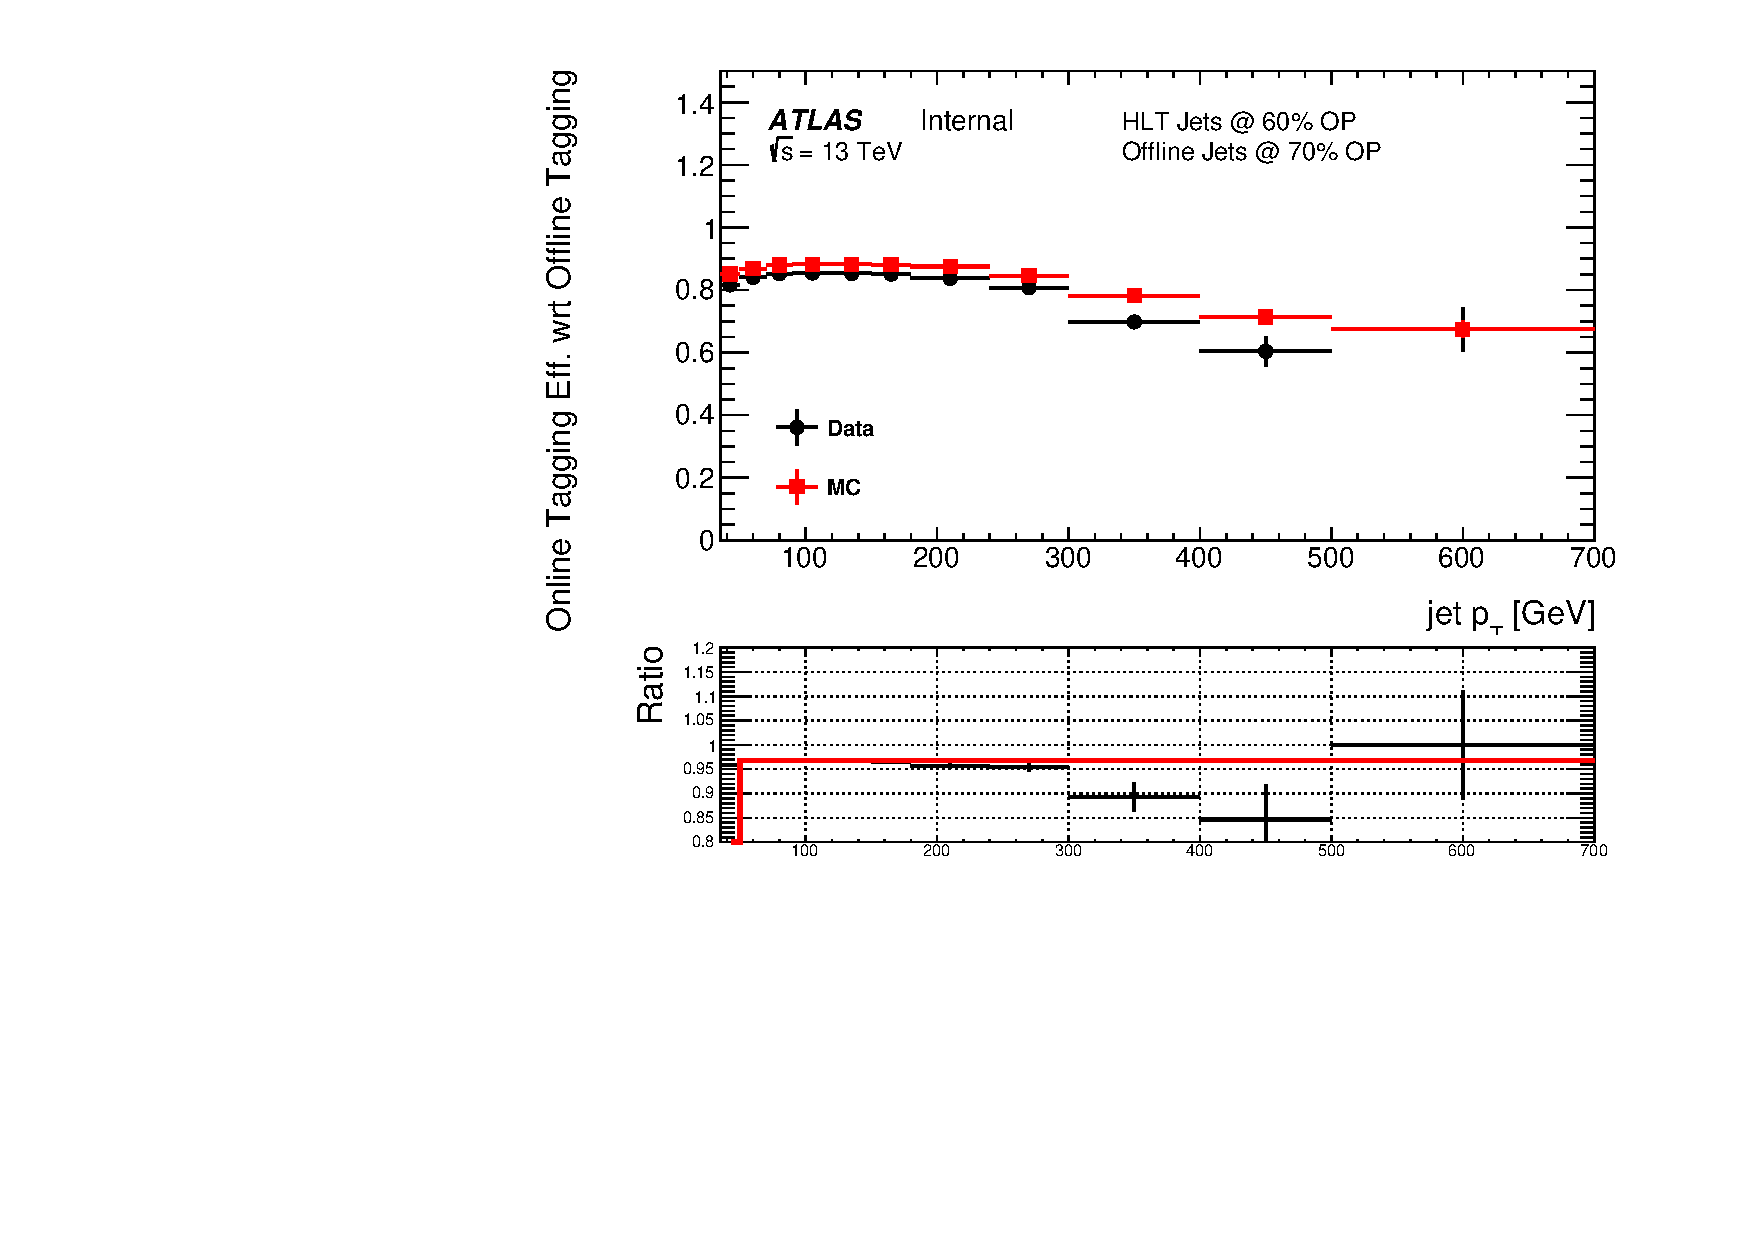
\includegraphics[width=0.47\linewidth, angle=0]{figs/Trigger/btrigger_old/Full_GRL_bslt2mm_trigReq_effFit_jetPt.pdf} }
  \subcaptionbox{Data/normalised MC with linear correction fit} {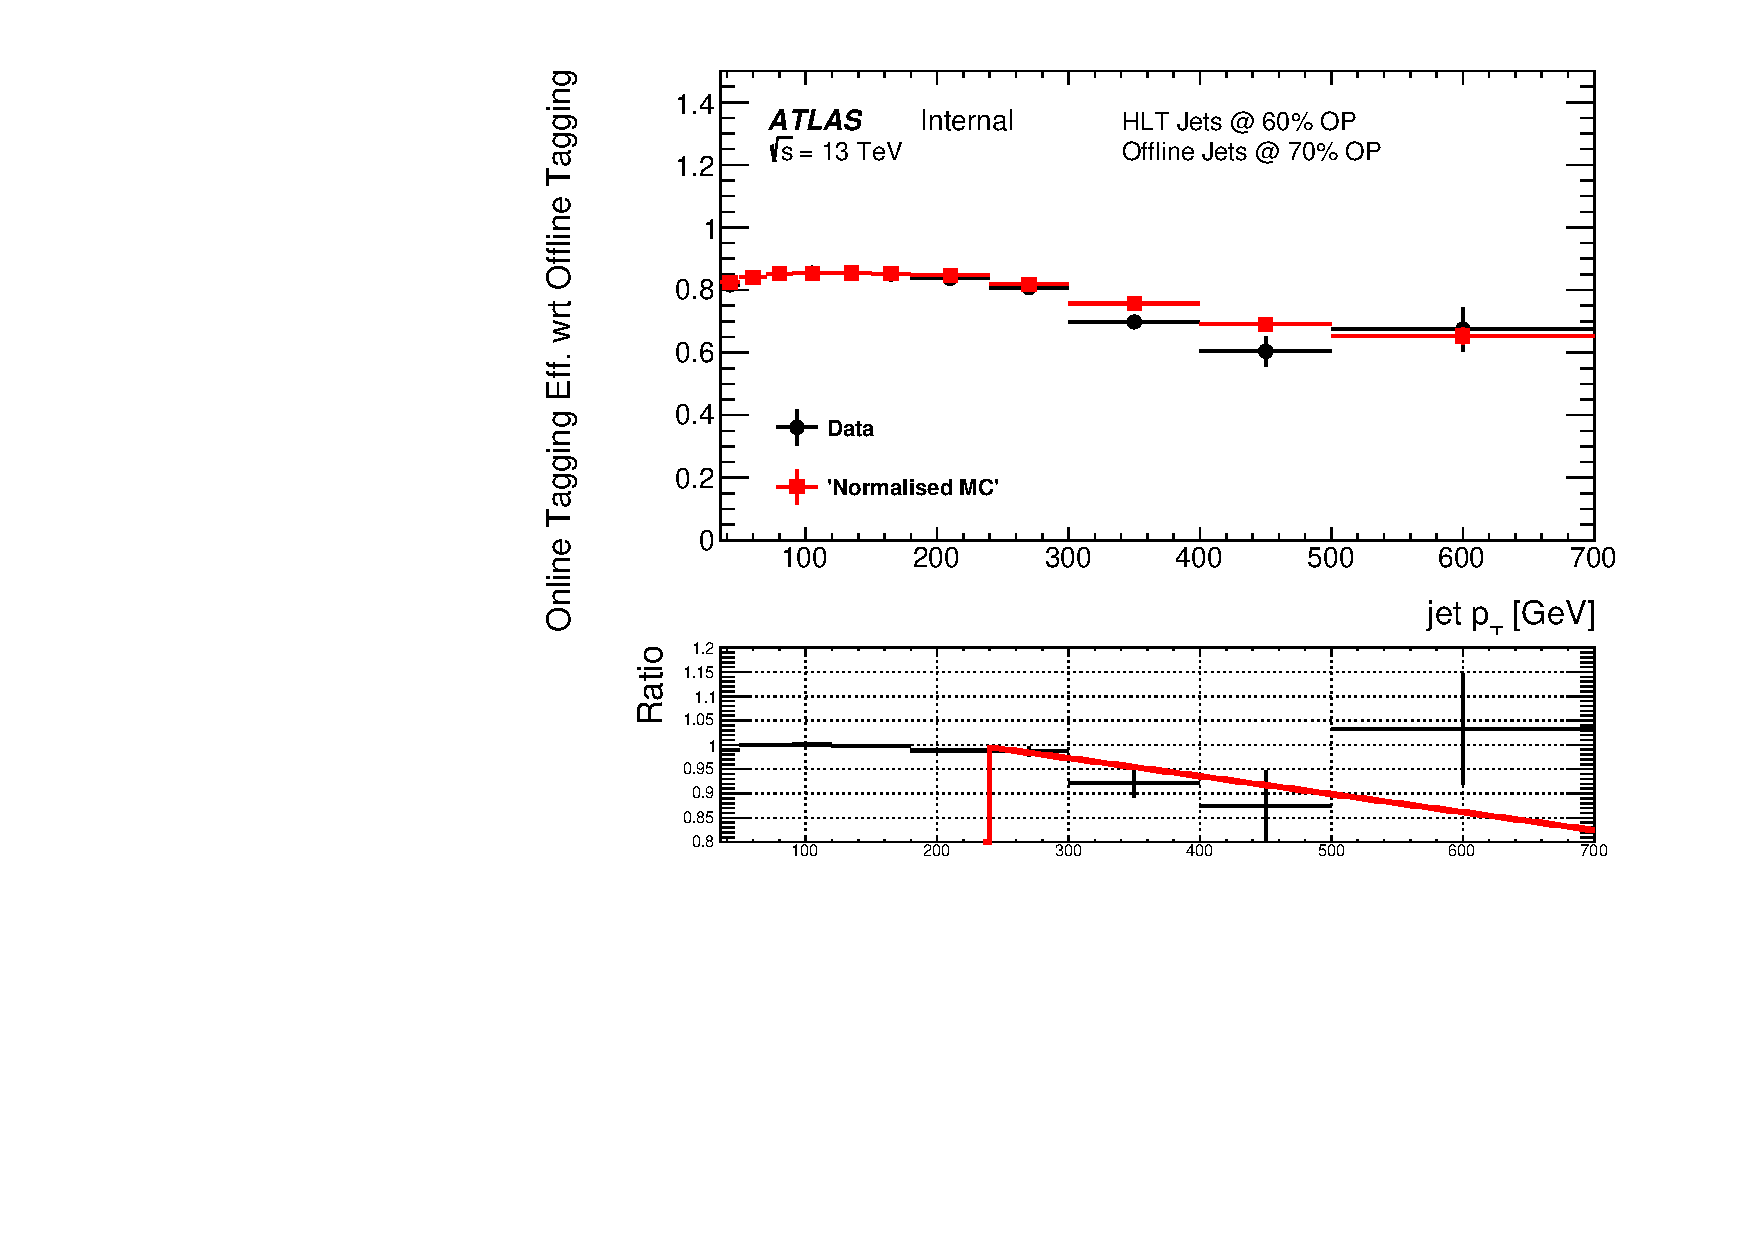
\includegraphics[width=0.47\linewidth, angle=0]{figs/Trigger/btrigger_old/Full_GRL_bslt2mm_trigReq_effNormFit_jetPt.pdf}} \\
  \subcaptionbox{Data/corrected MC with linear correction fit errors} {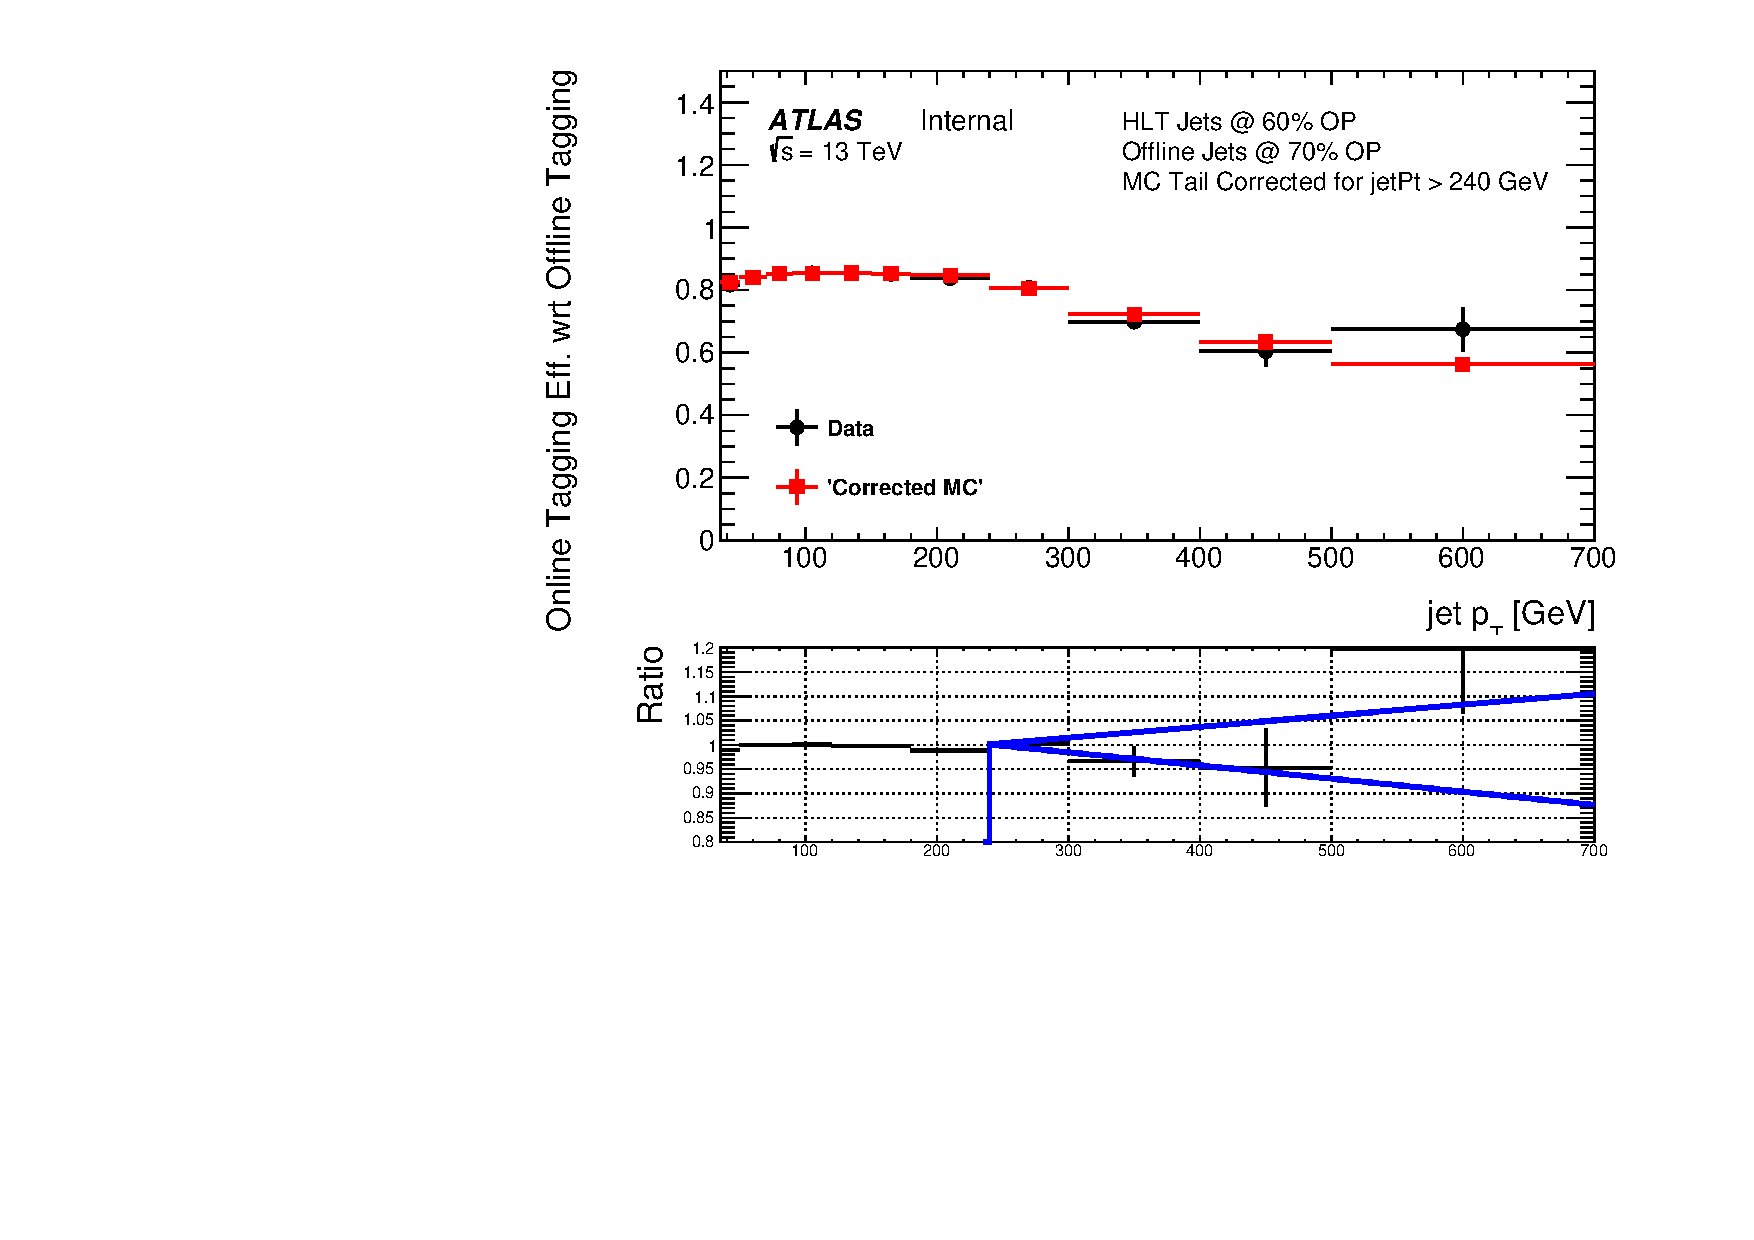
\includegraphics[width=0.47\linewidth, angle=0]{figs/Trigger/btrigger_old/Full_GRL_bslt2mm_trigReq_effCorrShapeErr_jetPt.pdf}}
  \subcaptionbox{Data/corrected MC with quadratic fit } {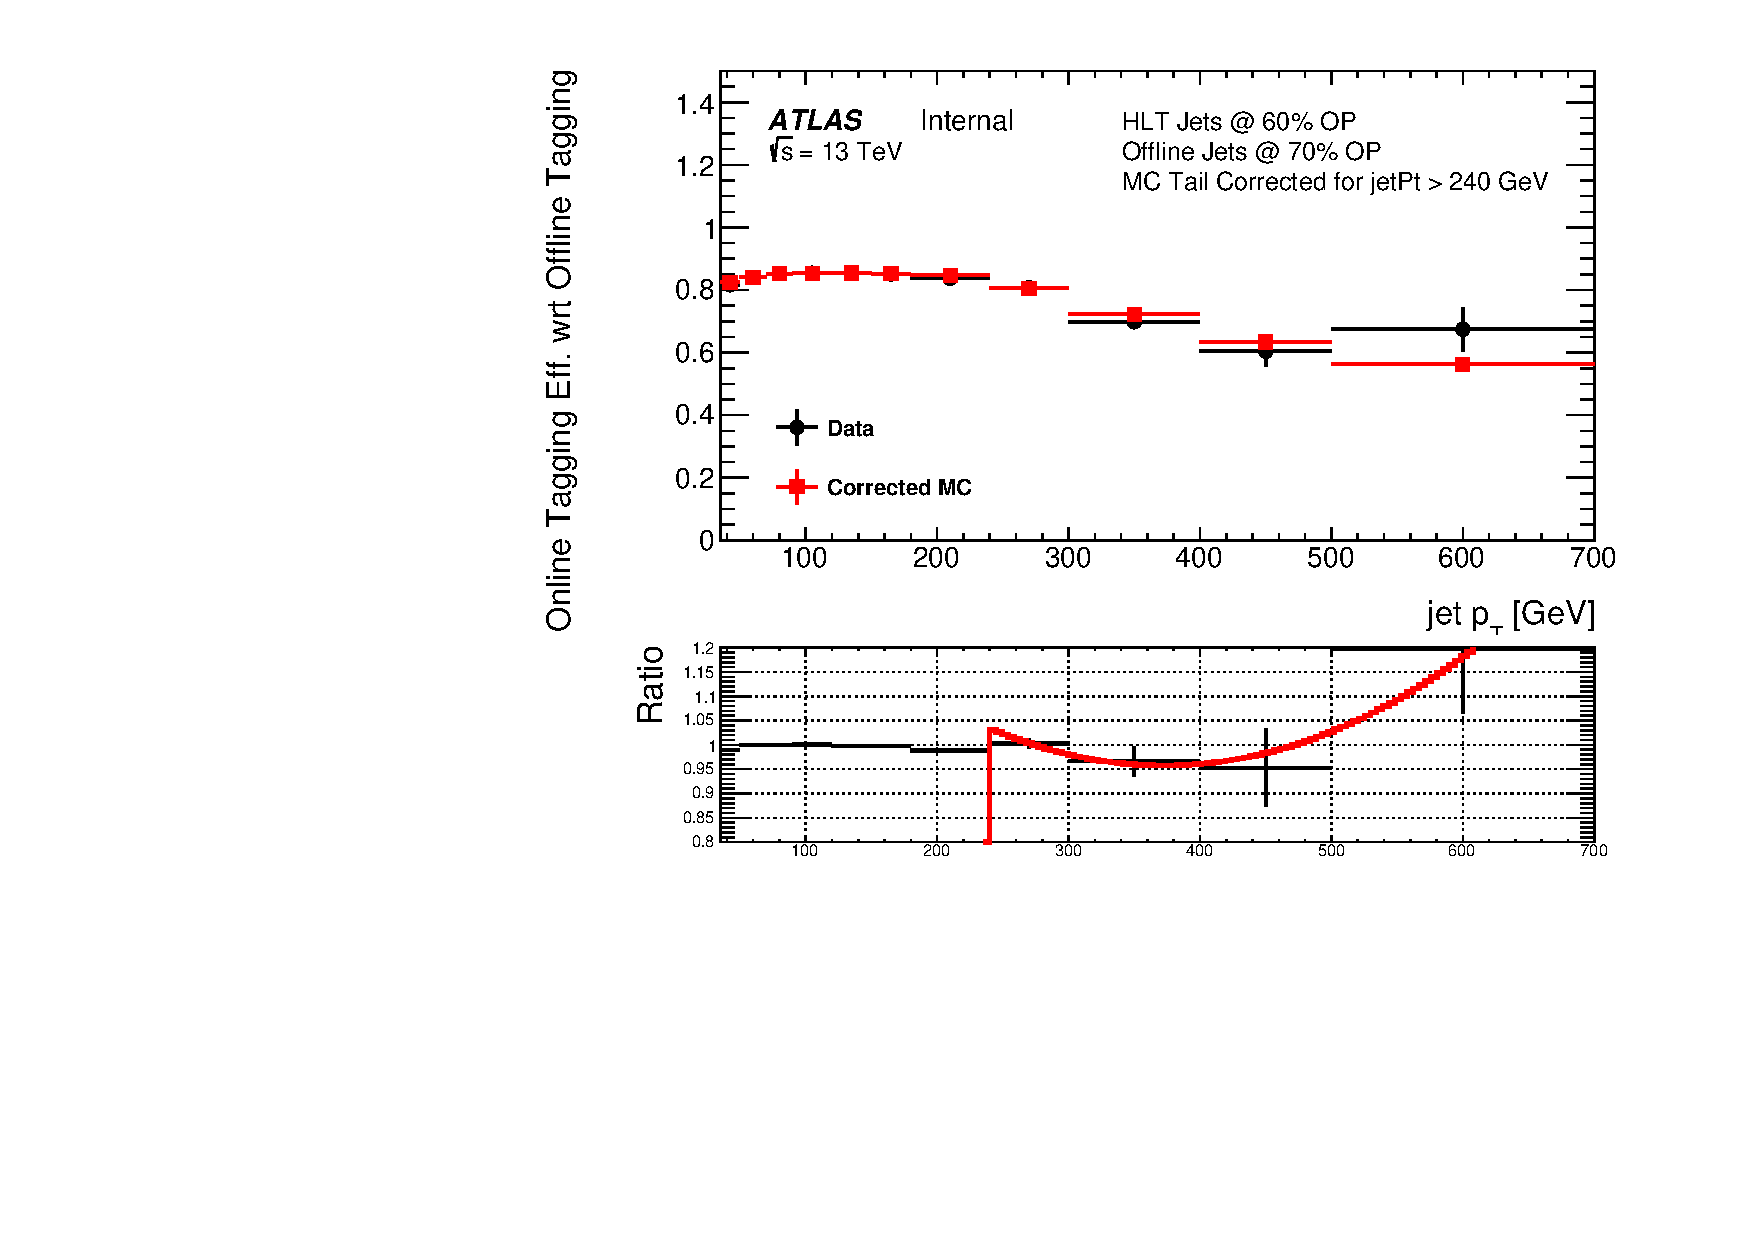
\includegraphics[width=0.47\linewidth, angle=0]{figs/Trigger/btrigger_old/Full_GRL_bslt2mm_trigReq_effCorrFitQuad_jetPt.pdf}}
\end{center}
\caption{A figure to demonstrate the high-\pT~extrapolation procedure for the 60\% $b$-jet trigger efficiency with respect to an offline 70\% operating point tag.
  Data (black) is compared against simulation (red) after various corrections have been applied  as a function of jet-\pT.
  Panel (a) shows the the flat normalisation fit uncorrected simulation, panel (b) shows the linear correction fit to normalised simulation,
  panel (c) shows the linear correction fit errors to the corrected simulation and panel (d) shows the quadratic fit to the corrected simulation.
  }
\label{fig:bTrig_mcExtrap}
\end{figure}

\begin{table}[!ht]
\begin{tabular}{|c||c||c|c|c|c|}
  \hline
  Jet pT [GeV] & MC Extrap. Error (\%) & Norm Fit Err. (\%) & Lin. Fit (\%) & Quad. Fit (\%)\\
  \hline
  240.0-300.0 & 0.8 & 0.0  & 0.8 & 0.3\\
  300.0-400.0 & 4.0 & 0.0  & 2.9 & 4.0\\
  400.0-500.0 & 5.6 & 0.0  & 5.6 & 1.7\\
  500.0-700.0 & 18.0 & 0.0 & 9.6 & 18.0\\
  \hline
\end{tabular}
  \vspace{10pt}
\caption{A table showing the systematic assigned for the high-\pT~extrapolation.}
\label{tab:bTrig_extrapSyst}
\end{table}

\FloatBarrier


\subsubsection{Jet-Level Efficiency and Scale Factor Measurement}
\label{sec:trig-jetLevelEff}

Now the raw measurements of $\epsilon_{bTrig}$ from Figure~\ref{fig:Full_bslt2mm_eff}
and the additional corrections and systematics described above can be brought together.
In Figure~\ref{fig:Full_bslt2mm_eff} it is shown that, whilst $\epsilon_{bTrig}$ does depend on jet-$\eta$,
the data to simulation ratio is flat with respect to jet-$\eta$.
However there is no significant dependence on jet-\pT~hence data/simulation scale factors are derived as a function of only jet-\pT. 

The full jet-level $\epsilon_{bTrig}$ measurement is shown in Figure~\ref{fig:bTrig_jetSys_eff}.
For use in combination with the simulation, a data/simulation scale factor as a
function of jet-\pT~is also derived and will be applied at the jet-level, which is also shown in Figure~\ref{fig:bTrig_jetSys_SF}.

The errors considered for the jet-level efficiency account for:
mismodelling of the b-jet purity in simulation, mismodelling of the b-jet trigger efficiency for non b-jets,
simulation statistical error , data statistical error (jet-$p_T <$ 240 \GeV) and simulation based extrapolation (jet-$p_T >$ 240 \GeV).
Table~\ref{tab:bTrig_jetSys} summarises the errors on the jet-level scale factor.
These errors are taken as a symmetric error in each jet-\pT~bin and the scale factors are applied to each b-tagged jet.\\

As a final sanity check Figure~\ref{fig:bTrig_jetSys_effComp} shows $\epsilon_{bTrig}$ measured in data to
that from the corrected simulation, in the lower panel a ratio of data to corrected simulation is shown
and the extrapolation and total errors are overlaid in red and green respectively.
The derivation of the corrected simulation and associated extrapolation errors is described in Section~\ref{sec:trig-highPtExtrap}
This shows that the corrected simulation lies within the total errors for the whole range of jet-\pT~
and at high-\pT, as one might expect, the error is dominated by the extrapolation uncertainties.
Note that the corrected simulation is only used to represent data for jet-\pT $>$ 240 \GeV.

\begin{figure}[!ht]
  \begin{center}
    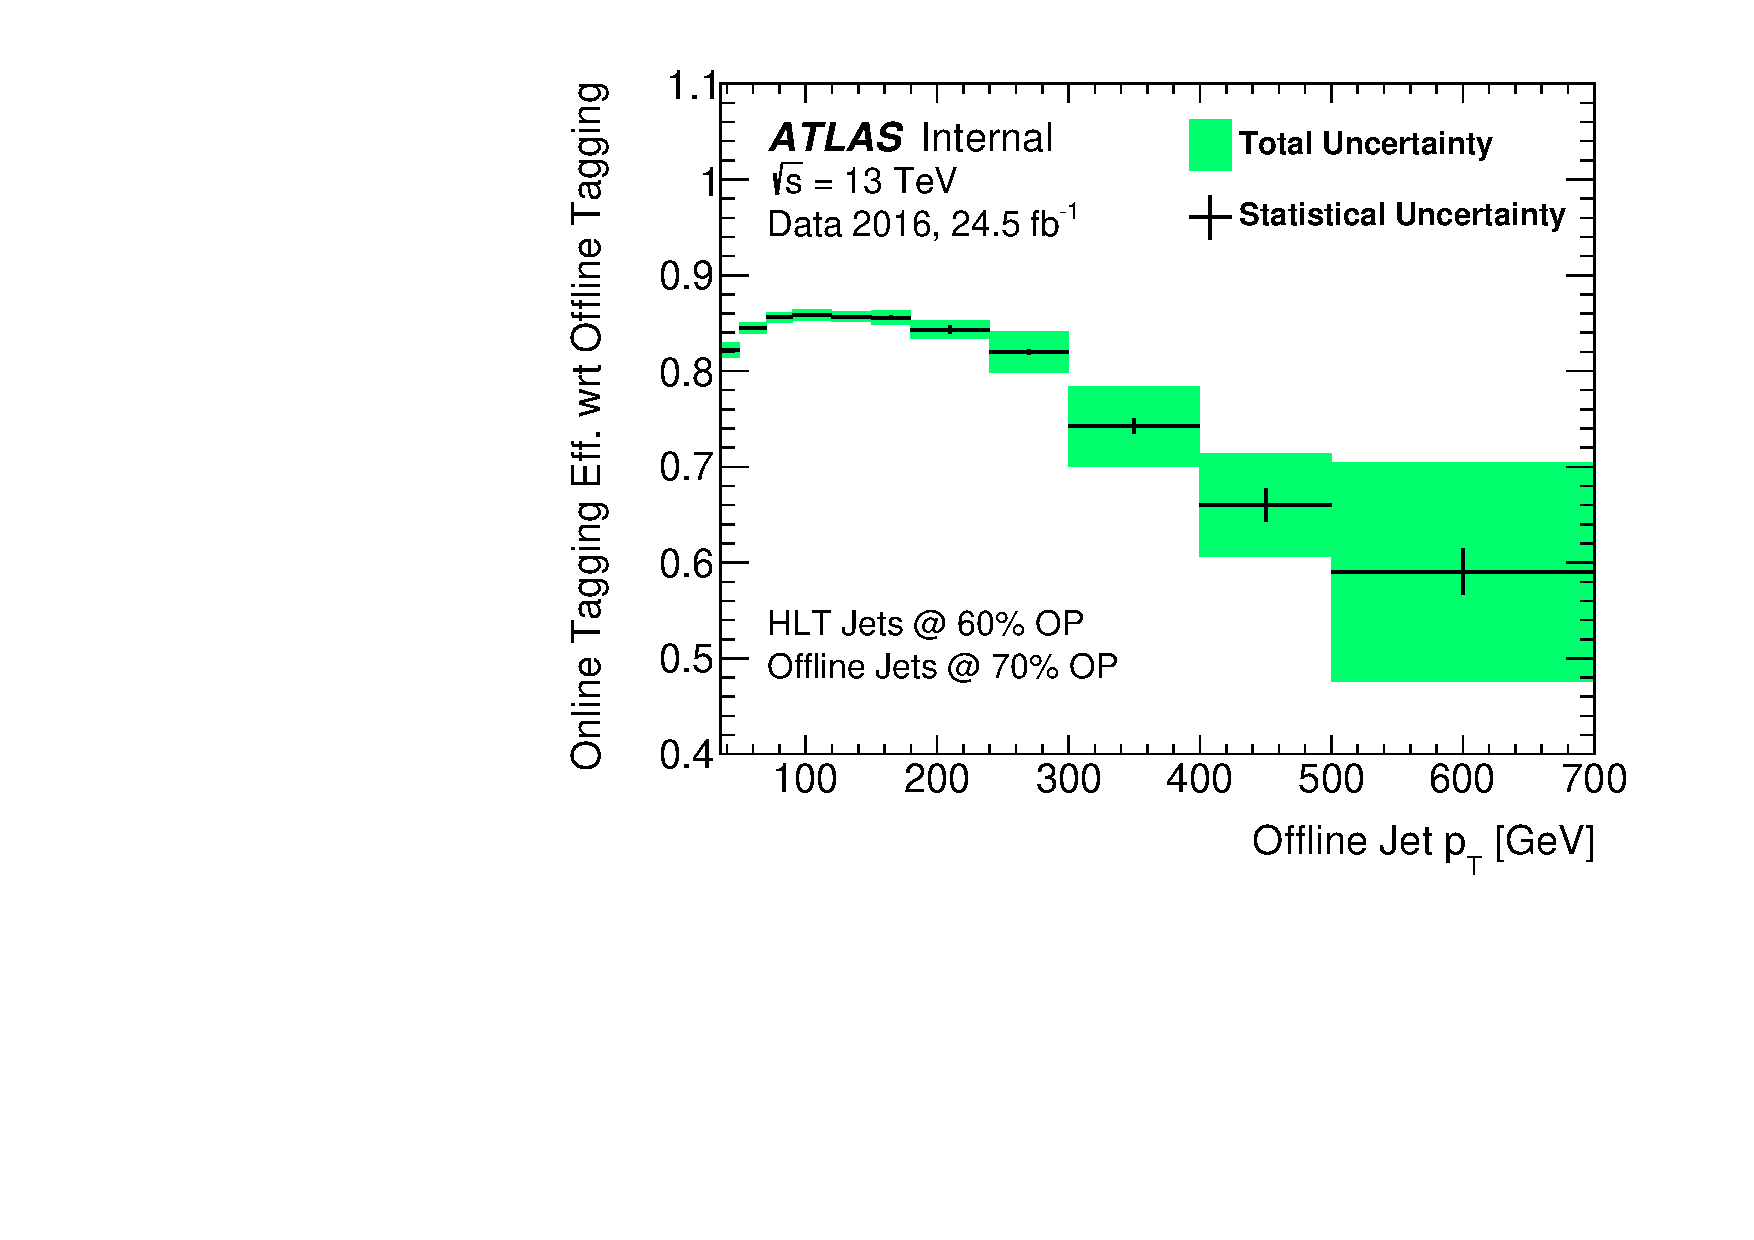
\includegraphics[width=0.8\linewidth, angle=0]{figs/Trigger/btrigger_old/fullSyst_Efficiency_jetPt.pdf}
  \end{center}
  \caption{
    The measured 60\% $b$-jet trigger efficiency with respect to an offline 70\% operating point tag
    as measured in data as a function of offline jet-\pT.
    The central values are shown in black with the statistical error and the green bands represent the total error including systematic errors.
    \label{fig:bTrig_jetSys_eff}
  }
  \begin{center}
    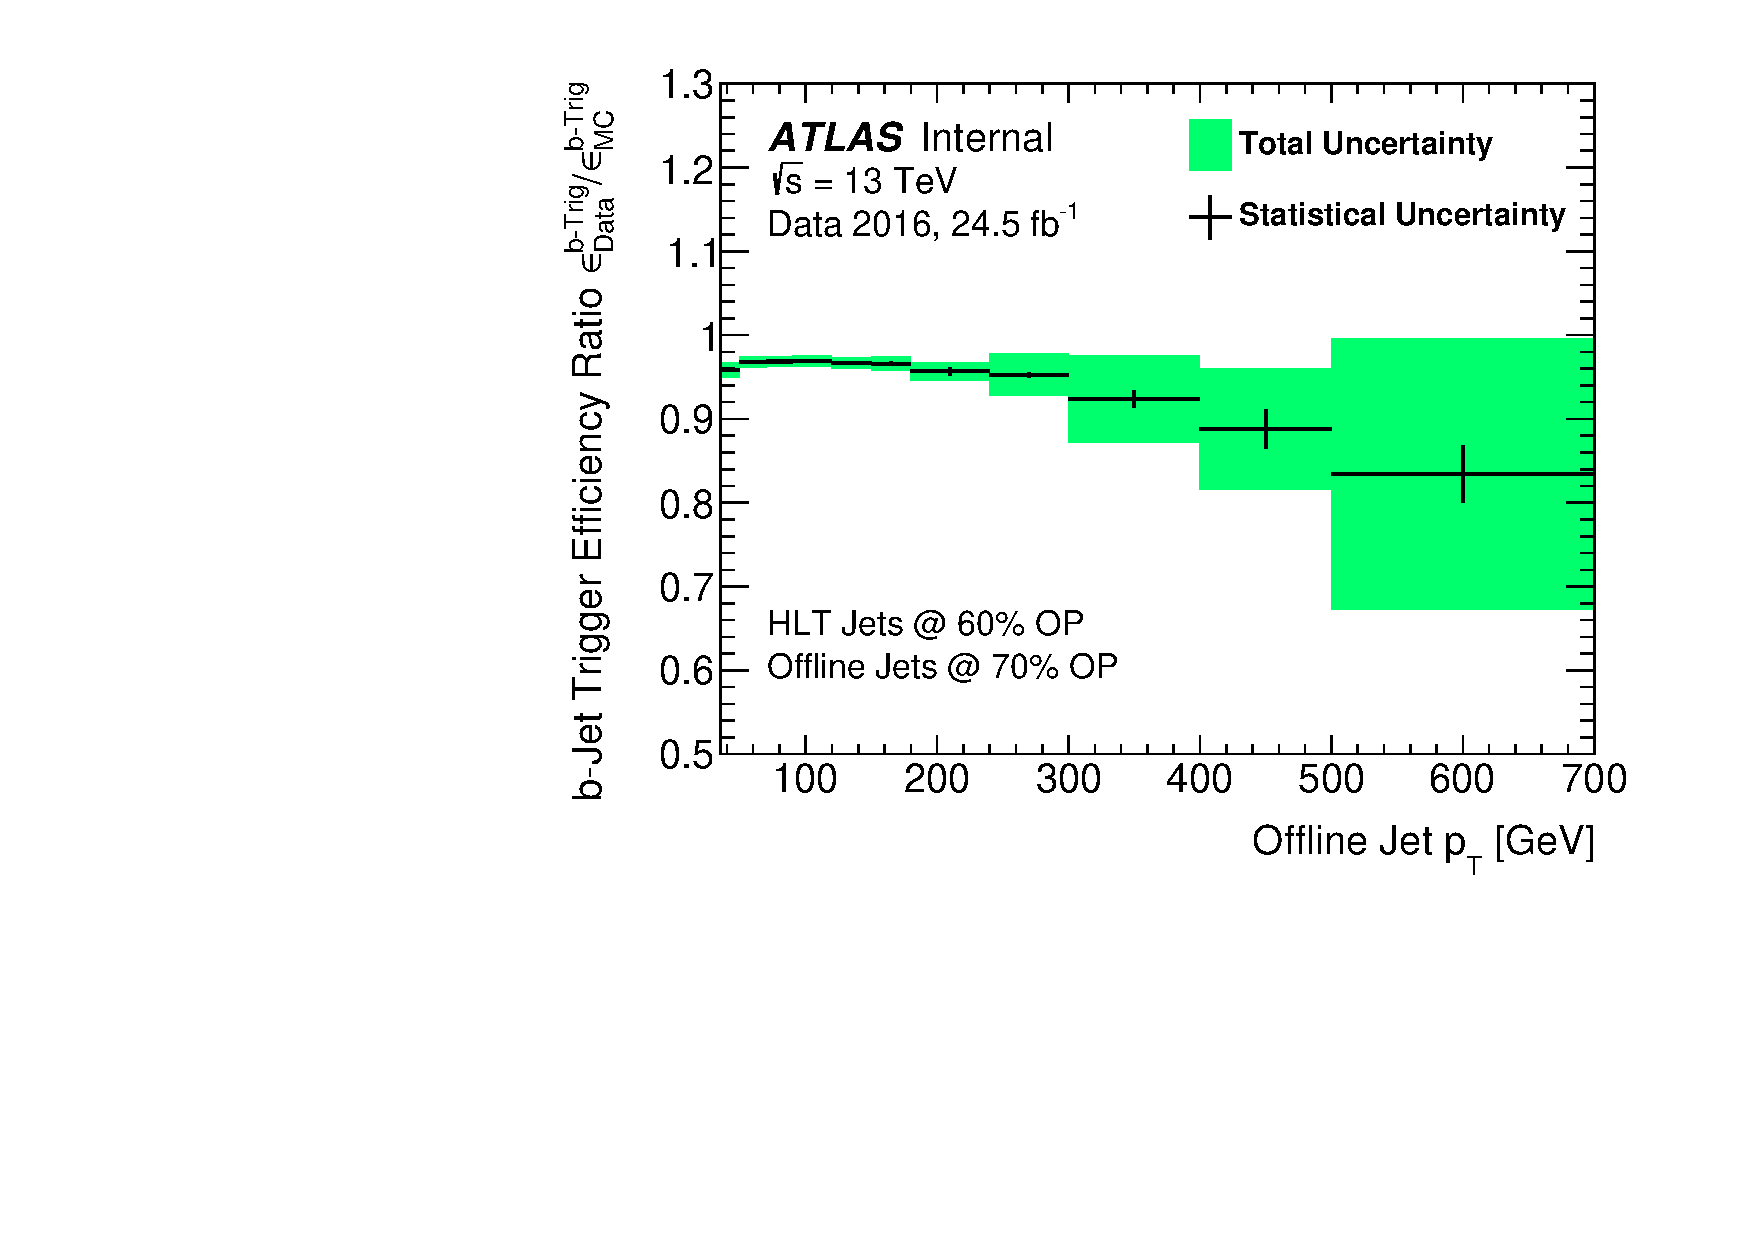
\includegraphics[width=0.8\linewidth, angle=0]{figs/Trigger/btrigger_old/fullSyst_ScaleFactor_jetPt.pdf}
  \end{center}
  \caption{
    Data/simulation scale factors for the 60\% $b$-jet trigger efficiency with respect to an offline 70\% operating point tag
    as a function of offline jet-\pT.
    The central values are shown in black with the statistical error and the green bands represent the total error including systematic errors.
    \label{fig:bTrig_jetSys_SF}
  }
\end{figure}

\begin{table}[!ht]
  \begin{tabular}{|c||c|c||c|c|c|c|}
    \hline
    Jet $p_T$ [GeV] & SF & Total Err. (\%) & Stat. (\%) & Extrap. (\%) & Pur. (\%) & L. Trig. Eff. (\%)\\
    \hline
    35.0-50.0 & 95.9 & 1.0 & 0.1 & - & 0.7 & 0.7\\
    50.0-70.0 & 96.8 & 0.7 & 0.1 & - & 0.5 & 0.5\\
    70.0-90.0 & 96.9 & 0.6 & 0.1 & - & 0.5 & 0.5\\
    90.0-120.0 & 96.9 & 0.7 & 0.1 & - & 0.5 & 0.5\\
    120.0-150.0 & 96.7 & 0.6 & 0.2 & - & 0.4 & 0.4\\
    150.0-180.0 & 96.6 & 0.9 & 0.2 & - & 0.6 & 0.6\\
    180.0-240.0 & 95.7 & 1.1 & 0.5 & - & 0.7 & 0.7\\
    \hline
    240.0-300.0 & 95.3 & 2.6 & 0.4 & 0.8 & 1.8 & 1.7\\
    300.0-400.0 & 92.4 & 5.6 & 1.1 & 4.0 & 2.8 & 2.5\\
    400.0-500.0 & 88.8 & 8.1 & 2.6 & 5.6 & 4.2 & 3.3\\
    500.0-700.0 & 83.4 & 19.4 & 4.0 & 18.0 & 4.9 & 3.1\\
    \hline
\end{tabular}
  \caption{A table showing the jet-level Data/simulation scale factor (SF) as a function of jet-$p_{T}$
    with total error and the contributions of the different systematics considered;
    specifically statistical, high-\pT~extrapolation, non-$b$-jet purity and non-$b$-jet trigger efficiency.}
\label{tab:bTrig_jetSys}
\end{table}

\begin{figure}[!ht]
  \begin{center}
    \includegraphics[width=0.8\linewidth, angle=0]{figs/Trigger/fullSys_EfficiencyComp_jetPt.eps}
  \end{center}
  \caption{
    The measured 60\% $b$-jet trigger efficiency with respect to an offline 70\% operating point tag
    as measured in data (black) and from the corrected simulation (red) as a function of offline jet-\pT.
    In the ratio plot on the lower panel the extrapolation errors is represented by the red band, whilst the total error is overlaid in green.
    \label{fig:bTrig_jetSys_effComp}
  }
\end{figure}

\FloatBarrier
\newpage

\subsubsection{Event-Level Efficiency and Systematic}
\label{sec:trig-eventLevelEff}

As alread discussed, in some regions of data-taking the performance
b-jet trigger efficiency itself
depends on the online beamspot position.
Hence, a b-jet trigger aware GRL is applied to remove a large fraction of
events where poor b-jet trigger performance is observed.

However, even after the application of this GRL,
there remains a bias with respect to leading jet-$\eta$ in the
probability of finding a valid primary vertex, which is notated as $\epsilon_{bPerf}$.
This bias is shown in Figure~\ref{fig:Full_bslt2mm_bperf}.
This efficiency is measured differently in each epoch,
in Epoch 1 it can be found as the number of events with vertex class = 0 divided by the number of events,
in Epoch 2 it is defined as the dividing the number of events that pass the trigger
\verb|HLT_mu26_imedium_2j35_bperf| by the number that pass the trigger \verb|HLT_mu26_imedium|
and in Epoch 3, due to the back-up vertex.
It should be noted that this measurement made in each of the three regions separately and is then combined with each region weighted by its luminosity.

The value of $\epsilon_{bPerf}$ is extremely close to 1 in simulation, in this case the efficiency in data and the scale factor are the same.
To assign a systematic for this correction the statistical error in data and simulation in addition to a shape systematic are used.
The shape systematic, to account for possible variations of the shape with respect to jet-$\eta$,
is defined as half of the difference between the maximum efficiency and the minimum efficiency in any jet-$\eta$ bin,
which effectively covers a flat distribution with respect to jet-$\eta$ to one where the shape is twice is extreme as observed.

Table~\ref{tab:bTrig_eventEff} and Figure~\ref{fig:bTrig_eventSys}
summarises the event-level efficiency correction and the associated systematics.

\begin{figure}[!ht]
  \begin{center}
    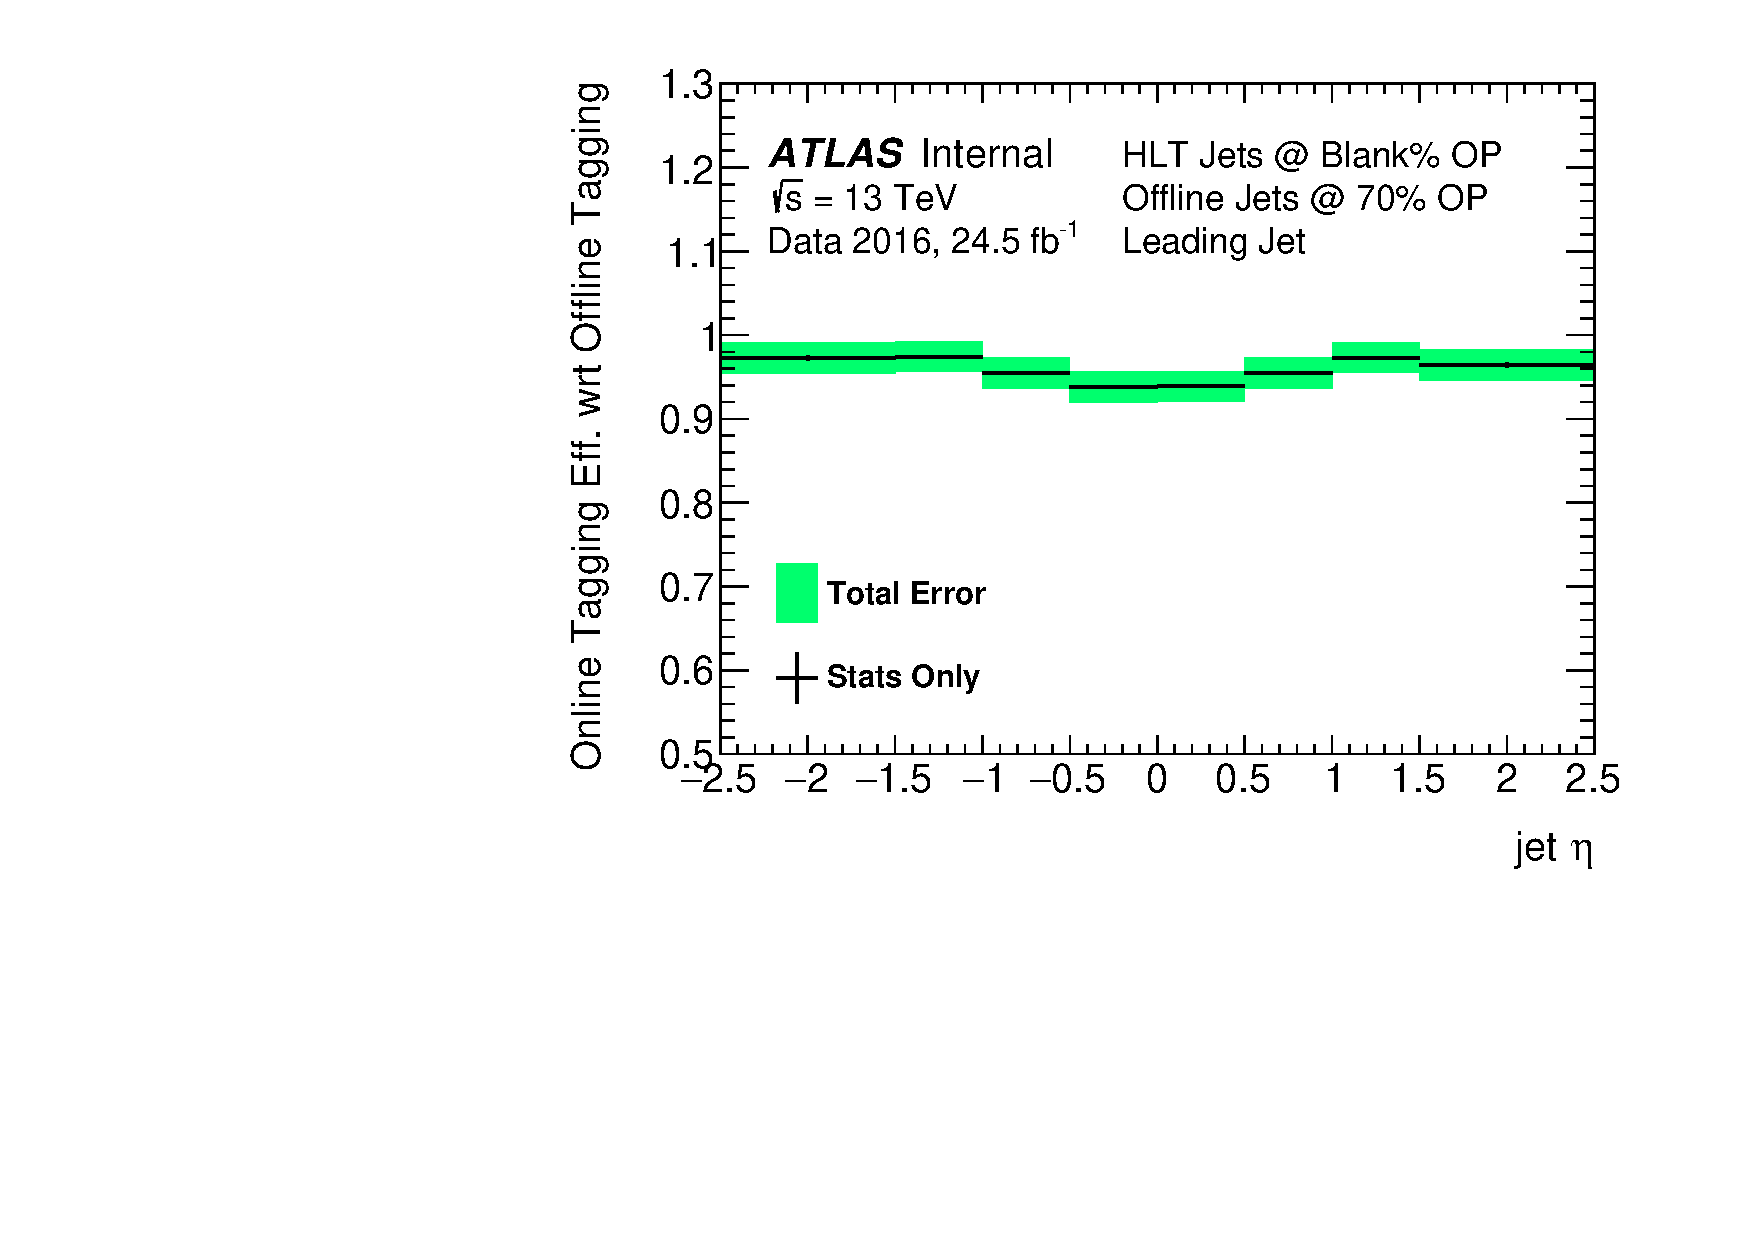
\includegraphics[width=0.8\linewidth, angle=0]{figs/Trigger/btrigger_old/fullSyst_EventEfficiency_leadingJetEta.pdf}
  \end{center}
  \caption{
    The measured $\epsilon_{bPerf}$ as measured in data as a function of offline leading jet-$\eta$.
    The central values are shown in black with the statistical error and the green bands represent the total error including systematic errors.
  }
  \label{fig:bTrig_eventSys}
\end{figure}

\begin{table}[!ht]
\begin{tabular}{|c||c|c||c|c|c||c|}
Leading Jet $\eta$ & SF & Total Error (\%) & Data Stat. (\%) & MC Stat. (\%) & Shape Syst. (\%)\\
\hline
-2.5--1.5 & 97.3 & 1.9 & 0.3 & 0.1 & 1.9 \\
-1.5--1.0 & 97.4 & 1.9 & 0.1 & 0.0 & 1.9 \\
-1.0--0.5 & 95.5 & 1.9 & 0.1 & 0.0 & 1.9 \\
-0.5-0.0 & 93.8 & 1.9 & 0.2  & 0.0 & 1.9 \\
0.0-0.5 & 93.9 & 1.9 & 0.2   & 0.0 & 1.9 \\
0.5-1.0 & 95.5 & 1.9 & 0.2   & 0.0 & 1.9 \\
1.0-1.5 & 97.3 & 1.9 & 0.1   & 0.0 & 1.9 \\
1.5-2.5 & 96.4 & 1.9 & 0.3   & 0.1 & 1.9 \\
\end{tabular}
\caption{A table showing the event-level Data/MC scale factor (SF) as a function of leading jet-$\eta$ with total error and the contributions of the different systematics considered.}
\label{tab:bTrig_eventEff}
\end{table}

\FloatBarrier
\newpage

\subsection{Cross-checks}
\subsubsection{Simulation checks}
- Ttbar alone vs ttbar+tW\\
- Try powheg
\subsubsection{Electron/Muon overlap checks}
\subsubsection{Event Level Eff: Showing correlation with $z_{bs}^{online}$}
- Show that it comes from high beamspot z-position only.\\
- i.e. $\epsilon_{bPerf}$ vs eta for different bs regions.
\subsubsection{Event Level Eff: Re-weighting of sub-leading jet}
- We did a test where we applied correction to leading and showes the subleading was flat within systematics (2\%)

Any others that are good?

Cross-checks can be moved to appendix

\section{To Do}

These can be considered on my list.
\noindent
- Cite in plot caption\\
- Uncertainty instead of error\\
- Update plots to most current version (and label those that are not)\\
- In caption I want (a) befor plot i.e. (a) jet-pT, (b) jet-eta.
- Always use data/simulation instead of data/MC\\
- use Epoch instead of epoch\\
